 %	Dies ist eine Vorlage von Tobias Banaszak  
%	tobias.banaszak@gmail.com
%	Einen Umschlag/Einband liefert diese Vorlage nicht, da die Schriftart der FH Aachen nicht mal so eben in *TeX genutzt werden kann und es genau daf�r in diesem Fall schon eine Indesign-Vorlage gibt
% 
\documentclass[
12pt,								% Schriftgre (12pt, 11pt (Standard))
oneside,							% einseitiges Layout
listof=flat,						% setzt z.B. das Abbvz neu, falls die Nummern in die Beschreibung rein ragt
%draft,								% �berlange Zeilen in Ausgabe kennzeichnen, setzt keine Bilder un Listings.
numbers=noenddot,		% macht aus der �berschrift 1.1. den letzten Punkt weg
%abstracton						%setzt "abstact"/"zusammenfassung"
]{scrartcl}
% 
%%%%%%%%%%%%%%%%%%%%%%%%%%%%%%%%%%%%%%
% Pakete einbinden etc...
%
%
%	Microtype macht einige Sachen etwas sch�ner. Sie dazu die Paketbeschreibung
\usepackage[protrusion=true,expansion=true,final]{microtype}
%
%
%	Blindtext
\usepackage{blindtext} %um mit leerem text zu f�llen
%Ben�tigt um Kopfzeile je nach Kapitel zu setzen
\usepackage{xifthen}
%
%
%\usepackage[numbers,round]{natbib}
%	Coole Kopfzeilen
\usepackage{fancyhdr}
\pagestyle{fancy}	
%
%	Kolumnentitel ohne Nummer davor
\renewcommand{\sectionmarkformat}{}
%
%	Alle Felder l�schen
\fancyhf{}	
%
%	Kopfzeile nicht in Grossschrift und ohne Nummerierung
\renewcommand{\sectionmark}[1]%
	{\markboth{ {} #1}{}}
\renewcommand{\subsectionmark}[1]%
	{\markright{ {} #1}{}}
%
%	Keine Linie zur Abtrennung der Kopfzeile
\renewcommand{\headrulewidth}{0mm}
%
%	Header
\fancyhead[R]{\parbox{\textwidth}{
	\begin{flushright}\small
		\textbf{\nouppercase\leftmark\phantom{\hspace*{1mm}}}{\textbar}\\%
		\vspace*{-1.1mm} %zeilenabstand etwas k�rzen
		%zweite Zeile:		
		\ifthenelse{\dimtest{\widthof{\rightmark}}{<}{3mm}}{\phantom{\textbar}}
		{\rightmark\hspace*{1mm}{\textbar}}
	\end{flushright}
}}
%
\fancyfoot[R]{\parbox{0.60\textwidth}{\begin{flushright}%
\textbf{\thepage}\hspace*{1mm}%
\end{flushright}}\hspace{0cm}}		% Seitenzahl rechts bzw. links unten
%
%
%	1,5facher Zeilenabstand
\usepackage{setspace}
\onehalfspacing
%
%
%	Deutsche Anpassungen
\usepackage[english]{babel}
\usepackage[ansinew]{inputenc} %iso 8859-1 (latin-1) als standart
\usepackage{scrhack}
%das funktioniert mit Windows gut
%
%
% Packages f�r Grafiken & Tabellen
\usepackage{graphicx} 			%Zum Laden von Grafiken
\usepackage{ctable}				%bunte Tabellen
%
%
%	Hyperref (klickbare Links im PDF)
%\usepackage[bookmarksnumbered,draft]{hyperref} 
\usepackage[bookmarksnumbered,final]{hyperref} %links ins web und innerhalb des pdf
%%f�r den Druck diese Zeile nutzen, damit die Links nicht gesetzt werden
%\usepackage[bookmarksnumbered,ocgcolorlinks,  linkcolor=black,        citecolor=black,        filecolor=black,        urlcolor=black,]{hyperref}
%
%
%	Bricht URLs um, besonders im Literaturverz. f�r den Druck auskommentieren
%	War in meiner alten Vorlage drin, scheint man mit einem aktuellen hyperref-Paket nicht mehr zu brauchen (es sei dennm man setzt �ber DVI und PS nach PDF und nicht mit PDFLaTeX)
% \usepackage{breakurl}
%
%
%	Mehrere Bilder in einer Figure
\usepackage{subfigure}
%
%
%	Farben
\usepackage{color}
\definecolor{DarkGrey}{cmyk}{0,0,0,0.75} % f�r Marginalien
\definecolor{mint}{cmyk}{1, 1, 1, 1} %FH-Mint mit 25% Schwarz, da es bei der d�nnen Schrift sonst sehr unter geht.
%
%
%	Listing-Umgebungen
\usepackage[final]{listings}		%Quellcode-Listings. final, damit die auch bei draft gesetzt werden
\usepackage{marvosym}			%paket, f�r das Enter-Symbol
%Javascript
\lstdefinelanguage{JavaScript}{
  keywords={typeof, new, true, false, catch, function, return, null, catch, switch, var, if, in, while, do, else, case, break, document, innerHTML, getElementById}
  keywordstyle=\color{blue}\bfseries,
  ndkeywords={class, export, boolean, throw, implements, import, this},
  ndkeywordstyle=\color{darkgray}\bfseries,
  identifierstyle=\color{black},
  sensitive=false,
  comment=[l]{//},
  morecomment=[s]{/*}{*/},
  commentstyle=\color{purple}\ttfamily,
  stringstyle=\color{red}\ttfamily,
  morestring=[b]',
  morestring=[b]"
}
%
%
%	F�r \floarbarrier, damit man floating-Objekte aufhalten kann (z.B. vor einer neuen section alle floats setzen)
\usepackage{placeins}
%
%
%	Dinge
\clubpenalty = 10000 % schliesst Schusterjungen aus
\widowpenalty = 10000 % schliesst Hurenkinder aus
%
%
%	Um das Logo absolut zu Posistionieren
%	In dieser Vorlage wird das FH-Logo nicht mehr benutzt, weil es auf den Umschlag kommt
%\usepackage[absolute]{textpos}
%\setlength{\TPHorizModule}{1mm}
%\setlength{\TPVertModule}{\TPHorizModule}
%\textblockorigin{0mm}{0mm}
%
%
%	Absatzeinzug verkleinern (bzw. eliminieren)
\setlength{\parindent}{0cm} 
%
%
%	Abk�rzungsverzeichnis
\usepackage[smaller]{acronym} 
%	Siehe dazu: http://www.matthias-schlecker.de/acronym-abkuerzungsverzeichnis-mit-latex-automatisieren
% 
%
%	Manuelle Worttrennung
\hyphenation{Ad-mi-nis-tra-tor Get-Re-quest Get-Re-sponse  Get-Next-Request Get-Bulk-Request Pro-gram-mie-rung fast-ether-net hexa-de-zi-mal-en}
%	Funktioniert trotzdem nicht mit Umlauten. Da dann im Text so trennen: �ber\-nahme\-er\-kl�rung
%
%
%	�berschriften im FH-Aachen-Mint
\addtokomafont{section}{\normalfont\Huge\color{mint}\hspace*{-0cm}} 
%
%
%	Abstand vor Kapitel�berschriften
\let\stdsection\section 
\renewcommand\section{\newpage\vspace*{1cm}\stdsection}
%
%
%	Ein wenig an der Geometrie herumzupfen um in die Vorlage zu passen
\usepackage{geometry}
%	Die auskommentierte Zeile nutzen um die Rahmen der Bereiche anzuzeigen
%\geometry{a4paper,left=2.7cm,right=6.7cm,top=2.0cm,bottom=4.4cm,marginparsep=7mm,marginparwidth=3.4cm,driver=pdftex,showframe}
\geometry{a4paper,left=2.7cm,right=2.7cm,top=2.5cm,bottom=4.4cm,marginparsep=7mm,marginparwidth=3.4cm,driver=pdftex}
%
%
%	Marginalien in grau und in kleiner
%\renewcommand\marginline[1]{%
%  \marginpar[{\begin{flushleft}\small\raggedleft\textcolor{DarkGrey}{#1}\end{flushleft}}]%
%            {{\small\raggedright\textcolor{DarkGrey}{#1}}}%
%}
%
%	Ich wei� nicht mehr, wozu ich das mal gebraucht habe. Eigentlich ist das die Aufgabe von Geometry. Daher erstmal auskommentieren
%\setlength{\headheight}{48pt}
%

\usepackage{ccicons}


\usepackage{booktabs}
%
\usepackage[T1]{fontenc}
%
%
%	Iwona-Schriften
\usepackage[light,math]{iwona}
\usepackage{amsmath}
%
\usepackage{longtable}
\usepackage{caption}

% Literaturverzeichnis-Header umdefinieren, damit oben rechts nicht zwei Mal "Literatur" steht
\makeatletter
\renewcommand*\bib@heading{%
  \section*{\bibname}%
  \@mkboth{\bibname}{}}%
\makeatother
%%%%%%%%%%%%%%%%%%%%%%%%%%%%%%%%%%%%%% 
%f�r den PDF-Reader
\hypersetup{
	pdfpagelayout=TwoPageRight,	%erste Seite ist Titelseite
	pdfstartview=Fit,
	pdfauthor={Tobias Augspurger}, 
	pdftitle={Range Imaging Applications for Dynamic Deformation Measurement},
	pdfsubject={Master's thesis},
	pdfkeywords={Time-of-Flight | Kinect 2 | Deformation | Dynamic}
}
%%%%%%%%%%%%%%%%%%%%%%%%%%%%%%%%%%%%%%
%
%
\begin{document}
%	Standartumgebung f�r Codelistings setzen
\lstset{showstringspaces=false,frame=lines,breaklines=true,language=[Sharp]C,numberbychapter=true,captionpos=b,prebreak={\Righttorque},basicstyle=\footnotesize}
%
%%%%%%%%%%%%%%%%%%%%%%%%%%%%%%%%%%%%%%
%%%%%%%%%%%%%%%%%%%%%%%%%%%%%%%%%%%%%%
%	Titelseite

\thispagestyle{empty}%
%\vspace*{6cm}
%\huge Master Thesis\newline%
%\rule{1mm}{100pt}


%\normalsize zur Erreichung des akademischen Grades \\
%\normalsize Master of Engineering\vspace*{0.5cm}
%
%\Huge \textcolor{mint}{\textbf{Konzeption und Entwicklung\newline einer multi-modalen\newline Connected-Mobility-App}}\vspace{2cm}
%\huge\textcolor{mint}{Range Imaging Applications for \\ %Dynamic Deformation Measurement}\newline
%\newline
%\huge Tobias Augspurger\vspace{2cm}

%\normalsize\textbf{University of Applied Science Aachen}\\
%{\color{mint}Aerospace Technology}\\

%\textbf{Author}\\
%Tobias Augspurger, B. Eng.\\
%Matriculation Number: 357059\\
%Aachen, \today\\

%\textbf{Examinant}\\
% Prof. Dr.-Ing. Harald Funke\\
%% 

\newgeometry{left=0.1cm,top=2cm,bottom=2cm,right=0.1cm}
\hbox{ % Horizontal box
    \hspace*{0.25\textwidth} % Whitespace to the left of the title page
    {\vrule}
    \hfill\begin{minipage}[b]{0.7\textwidth}
        \begin{minipage}[c]{.8\linewidth}
            \begin{center}
                \vspace{\baselineskip}
                {\Large \textsc{Fachhochschule Aachen}}

                {\large Fachbereich 6}

                {\large Luft- und Raumfahrttechnik}

                \vspace{6\baselineskip}
            \end{center}
        \end{minipage}\hfill\begin{minipage}[b]{.1\linewidth}
            \includegraphics[width=\linewidth]{Bilder/FH_logo.png}
        \end{minipage}

        \vfill
        \begin{center}
            \begin{minipage}{.7\textwidth}
                \centering
                {\Large\bfseries Master Thesis}

                \vspace{.8\baselineskip}
                {\Huge Range Imaging Applications for Dynamic Deformation Measurement}
				
				 \vspace{7\baselineskip}
				 {\Large von}\\ % Author name
                {\Large Tobias Augspurger}\\ % Author name
                {\Large Matriculation Number: 357059}\\ % Author name
                \vspace{5\baselineskip}
                
                \begin{tabular}{l l}
                Referent: & \large Prof. Dr.-Ing. H. Funke\\
                Korreferent: & \large Prof. Dr.-Ing. B. Burbaum
                \end{tabular}
            \end{minipage}
        \end{center}
    \end{minipage}
}
\restoregeometry
%

% Seitengeometrie f�r den Titelseite & Verzeichnisse anpassen
\newgeometry{left=2.7cm,right=2.7cm,top=3.05cm,bottom=3.3cm,marginparsep=0mm,marginparwidth=0.0cm}
\onehalfspacing
\newpage
\section*{Erkl�rung}
Ich versichere hiermit, dass ich die vorliegende Arbeit selbstst�ndig verfasst und keine anderen als
die im Literaturverzeichnis angegebenen Quellen benutzt habe.\newline\newline
Stellen, die w�rtlich oder sinngem�� aus ver�ffentlichten oder noch nicht ver�ffentlichten Quellen
entnommen sind, sind als solche kenntlich gemacht.\newline\newline
Die Zeichnungen oder Abbildungen in dieser Arbeit sind von mir selbst erstellt worden oder mit
einem entsprechenden Quellennachweis versehen.\newline\newline
Diese Arbeit ist in gleicher oder �hnlicher Form noch bei keiner anderen Pr�fungsbeh�rde eingereicht
worden.\newline\newline\newline
\par
Aachen, 26.1.2015
\newpage
\section*{Abstract}
Three-dimensional Time-of-Flight (ToF) range cameras improved significantly in accuracy, speed, price and size over the last years. By delivering the range from the scene to the image sensor in every pixel, static and dynamic scenes can be reconstructed into a three-dimensional model contactless from a single point of view. The observed area is illuminated by infrared diodes and a IR CMOS camera measures the time delay of the returning light \cite{thierryoggietof}. Out of it the range is acquired parallel with no time delay between the pixels \cite{litime}. This offers the potential for various close to medium range applications. One of this is the measurement of vibrations and structural deformations under dynamic loads \cite{qi2014structural}. In contrast to other present measurement methods, complete surface movements can be acquired in parallel without a movable laser beam or a complex stereo triangulation between multiple cameras . The Kinect 2 range camera is used to show the performance of vibration measurements and to analyze how the range images can be filtered and processed. It is the first ToF camera on the consumer market and at the time of release the one with the highest number of pixels ($512x424$ at 30 frames per seconds). It delivers 3D informations from $0.6~m$ to $8.0~m$ at a depth resolution of $1~mm$ \cite{sell2014xbox}. A Laser Doppler Vibrometer is used, as high precision reference measurement device, delivering the highest standard in deformation measurement on a single surface point. This thesis will prove, that vibrations of a body can be reconstructed at amplitudes of $4~mm$ with an accuracy below $1~mm$. The performance depends on the distance to the camera, angle of view, surface material, number of investigated pixels and the measurement time. At the ideal distance of $1.3~m$ to $1.5~m$, the error to the reference is reduced down to $0.05~mm$ after 8 seconds of measurement at a frequency of $3~Hz$. Even the first and second harmonics are visible in the frequency domain on white paper, offering a high reflectivity for the infrared light of the ToF measurement principle. The influence on the accuracy of different angles to the surface normal is another topic. A vibration of $3~Hz$ can be reconstructed correctly in frequency up to an angle of $45^\circ$. The amplitude is overestimated with higher angles. Since every pixel delivers a range information, the complete video stream can be processed by a Fast-Fourier Transform to derive the dynamic behavior of the whole field of view. The vibration can be illustrated in images, representing the amplitude and frequency distribution in the complete field of view over a certain time span.\\

This development offers new applications in the static and dynamic observation and investigation of machines and structures. Positions, geometries, movements, orientations and other object properties can be analyzed and reconstructed in real time. Industrial installations and processes such as engines can be observed and the production quality can be improved.
\section*{Acknowledgment}
The work described in this thesis would not be possible without the extensive support from Prof. Funke and the team of propulsion laboratory at the University of Applied Science Aachen. From the rough idea to the finished experimental results I got a lot of support and feedback that helped me to find the right way even if the tasks seemed impossible to fulfill. Prof. Kameier from the University of Applied Science Duesseldorf delivered us a high precision reference measurement device. He also contributed Matlab source code that was necessary for the evaluation. I would also like to thanks Prof. Franke who allocated the oscilloscope for the acquisition of the Laser Doppler Vibrometer. Many thanks goes also to my family and friends, who supported me over the last months, corrected my texts and gave me a lot of feedback.  
\newpage
%%%%%%%%%%%%%%%%%%%%%%%%%%%%%%%%%%%%%%
%	Erzeugen von Verzeichnissen
\renewcommand{\listfigurename}{List of figures}
\markright{}%gegen die zweite zeile im header
\tableofcontents			% Inhaltsverzeichnis
\newpage
%
\markright{}					% gegen die zweite zeile im header
%\listoftables				% Tabellenverzeichnis
%\thispagestyle{empty}
\section*{List of Abbreviations}
\sectionmark{List of Abbreviations}

\begin{longtable}[l]{p{150pt} p{300pt}}
ToF	& Time-of-Flight\\
IR & Infrared\\
CMOS & Complementary Metal-Oxide-Semiconductor\\
LDV & Laser Doppler Vibrometer\\
VIS & Visible\\
UV & Ultraviolet\\
CIE & Commission International de l'Eclairage\\
LED & Light-Emitting Diodes\\
CRI & Color Rendering Index\\
RGB & Red, Green, Blue\\
CCD & Charged-Coupled Device\\
SPAD & Single-Photon Avalanche Diodes\\
ADC & Analog-to-Digital Converter\\
DNR & Dynamic Range\\
SNR & Signal-to-Noise Ratio\\
FOV & Field of View\\
LiDAR & Light Detection and Ranging\\
SAR & Synthetic Aperture Radar\\
CW & Continuous-Wave\\
FFT & Fast Fourier Transform\\
DFT & Discrete Fourier Transform\\
STFT & Short-Time Fourier Transform\\
HD & High Definition\\
AMP & Amplifier\\
TIFF & Tagged Image File Format\\
PCL & Point Cloud Library\\
STL & Surface Tesselation Language\\
TVD & Total Variation Denosing\\
CSV & Comma-Separated Values\\
PIV & Particle Image Velocimetry\\
BNC & Bayonet Neill Concelman\\
PSP & Pressure Sensitive Paint\\ 

\caption{List of Abbreviations}
\end{longtable} 

\begin{table}
\vspace{1 mm}  
\end{table}

\begin{table}
\vspace{1 mm}
\end{table}
\newpage
\section*{List of Symbols}
\sectionmark{List of Symbols}

\begin{longtable}[l]{p{150pt} p{150pt} p{200pt}}
\textbf{Symbol}	& \textbf{Units} & \textbf{Description} \\ 
c	& $m \cdot s^{-1} $	& Speed of light\\
$\vec{E}$	& $V\cdot m^{-1}$	& Electric field\\
$\vec{M}$	& $N\cdot m^{-1}\cdot A^{-1}$	& Magnetic field\\ 
$\lambda$	& $m$	& Wave length of light\\ 
$\nu$	& $Hz$	& Frequency of light\\ 
$E$ & $J$ 	& Energy\\
$P$ & $W$ & Power\\
$h$ & $6,626 069 57 \cdot 10^{-34} J\cdot s$ & Planck constant\\
$m$ & $kg$ & Mass\\
$\Phi _e$ & $W$ & Radiant flux\\
$\Phi _v$ & $lm$ & Luminous flux\\
$\Omega$ & $sr^{-1}$ &  Solid angle \\
$I_e$ & $W\cdot sr^{-1}$ & Luminous intensity \\
$\eta_v$ & $lmW^{-1}$ & Lumious efficacy\\
$\varrho$ & $\%$ & Reflectance\\
$\tau$ & $\%$ & Transmittance \\
$\alpha$ & $\%$ & Absorption \\
$U_{th}$ & V & Threshold voltage\\
$R_{\lambda}$  & $AW^{-1}$ & Resposivity \\ 
$Q.E.$ & $-$ & Quantum efficiency \\
$fps$ & $1/s$ & Frames-Per-Second\\
$t_r$ & $s$ & Response time \\
$t_e$ & $s$ & Exposure time \\
$F$ & $m$ & Focal length \\
$\theta$ & $DEG$ & Angle of View \\
$\vec{s}_{blur}$ & m & Motion blur\\
$\vec{v}$ & $ms^{-1}$ & Speed\\
$n$ & Hz & Rotational speed\\
$d$ & m & Distance\\
$t_{ToF}$ & s & Time-of-Flight \\
$f_{mod}$ & Hz & Modulation frequency\\
$\varphi$ & rad & Phase shift\\
$\sigma^2$ & - & Variance\\
$d_{amb}$ & - & Ambiguity distance\\
$n_{bits}$ & Bit & Bit depth\\
$\dot n $ & $\frac{bit}{s}$ & Data stream\\
$f_{sampling}$ & Hz & Sampling frequency\\
$f_{max}$ & Hz & Maximum frequency in signal\\
$f_{nyquist}$ & Hz & Nyquist-Shannon frequency\\  
$A$ & - & Amplitude\\
$A_{pp}$ & - & Peak-to-peak amplitude \\
$l_{hv}$ & m & Vertical / horizontal length \\   
$\nabla$ & - & Nabla operator\\
$\lambda_r$ & - & TVD regularization parameter\\
$U_{AC}$ & - & Alternate voltage\\
$E$ & $mm^{-1}s^{-1}V^{-1}$ & Sensitivity of LDV\\
$T_{sampling}$ & s & Time between two sample points\\
$ \vec{n}$ & - & Surface normal vector\\
$\alpha$ & $DEG$ & Viewing angle \\
$\beta $ & $DEG$ & Cone angle of membrane\\
\caption{List of symbols}
\end{longtable} 

\begin{table}
\vspace{1 mm}  
\end{table}

\begin{table}
\vspace{1 mm}
\end{table}
\newpage
%
%%%%%%%%%%%%%%%%%%%%%%%%%%%%%%%%%%%%%% 
%%%%%%%%%%%%%%%%%%%%%%%%%%%%%%%%%%%%%%
%	Der Text
\restoregeometry			% Seitengeometrie zur�ck setzen
%\blinddocument
%
%	Motivation
\section[Introduction]{Introduction}\label{sec:motivation}
The interest in new innovative kinds of human/computer interaction lead to multiple low cost developments to detect the movement of a human body. The Kinect 2, developed by Microsoft, measures the propagation time of light by the Time-of-Flight (ToF) principle, to derive 3D data from the observed scene. The field of view is illuminated by IR didoes and a IR CMOS camera measures the time that the light take to reflect back into the camera. With the constant speed of light and the measured time of flight the distance, that the light traveled, can be calculated.  Since the appearance of ToF cameras in the year 2000, the pixel resolution, dynamic range and the accuracy have significantly improved. In contrast to stereo triangulation between multiple cameras or 3D scanning with a moving laser beam, this technique allows low cost and small size applications for 3D scanning. High frame rates can be achieved and the 3D data is acquired on every pixel at the same time.\\

 The acquisition of real-time 3D data also offers various applications in experimental setups. In crash test facility for example the geometry and orientation of the structures before and after the test can be measured. In windtunnel applications, the angle of attack and vibrations of the aerodynamic body can be observed by the camera without disturbing markers on the surfaces. The measurement of the static geometries and the dynamic behavior delivers a way to merge data between different calibrated camera systems in a common set of data. Aeroelasticity investigations are possible on the complete body in every point of the field of view.\\

 This thesis will reveal how static and dynamic ToF data can be investigated and processed. Xiao Qi and Derek Lichti already showed the performance of dynamic beam deformation measurement with ToF \cite{qi2014structural}. A $1~Hz$ sinus oscillation of an concrete beam with an amplitude $4~mm$ was reconstructed with an accuracy of $0.061~mm$. This was possible with two phase synchronized ToF cameras in a stereo arrangement for a single point on the beam. The noise and uncertainty between both sensors are canceled out between both measurements. The advantages of static investigation with a Time-of-Flight camera for structural deformation measurement have already been proven with last generation devices \cite{jamtsho2010geometric}. In previous investigations of 3D scanning techniques for static deformation, Terrestrial Laser Scanning also showed a high performance, but the systems are slow, expensive and large \cite{park2007new}.\\
    
 Advanced ToF image sensors with a higher pixel resolution, accuracy and improved noise characteristic promise the dynamic investigations of complete surfaces with a single camera. A depth resolution up to $0.3~mm$ is possible, with current CMOS technology \cite{yasutomi20147}. Other devices feature high frame rates of $470~fps$ in a 1280x1024 pixel area \cite{odosimagingdatasheet}. The dynamic performance of the Kinect 2 ToF camera, that is originally designed for human/computer interaction, will be investigated. The accuracy of the measurement will be compared to a Laser Doppler Vibrometer (LDV). A speaker membrane delivers a constant dynamic movement with a calibrated sinus function as input. Therefore, deformation measurement like Stereo Pattern Tracking can be investigated on a controlled test body \cite{mantik2013enhancement}. Boundary conditions like surface material, geometry and angle of the camera to the surface normal will be analyzed in terms of precision and accuracy. Another major advantage of range data is the simple image processing that will be shown in Matlab for some basic examples for the static and dynamic structure investigation. The creation of surface dynamics images, showing the frequency and amplitude distribution, is one of the main subjects in this context. This delivers a simple and easy way to obtain the dynamic behavior of complete surfaces. Applications of Time-of-Flight cameras are shown in multiple small experiments. The revealed procedures are only supposed to show the performance of the measurement principle in a rough way and demonstrate how a real calibration of the ToF System in a controlled environment can look like. ToF cameras have not been investigated previously at the Department of Aerospace Technology which offers the possibility to build up knowledge from a unprejudiced basis. The source code for image processing has been developed without any examples. Improvements are still necessary in the experimental setup, source code and suggested theories.     
%	Stand der Technik
\section{State of the Art}\label{chap:standdertechnik}
\subsection{The Fundamentals of Light}
Light is a substantial part of the universe. It lets us see the world, the stars and has remarkable properties in the space-time. For example it is the fastest way of energy transportation with a speed of $c = 299792458~m/s$ in vacuum. The definition of electromagnetic radiation gathers all kinds of light like visible (VIS), infrared (IR), ultraviolet light (UV) and other kinds of radiation like microwaves or radio waves. James Clerk Maxwell discovered that light can be described by an electric $\vec{E}$ and a magnetic $\vec{M}$ field that stand perpendicular to each other and to the direction of wave propagation. Figure \ref{fig:LightasWave} shows the propagation of one light ray. Both fields oscillated with the same wavelength of the light $\lambda$ and the frequency $\nu$ moving into the wave direction of the wave vector propagation. Green light for example is defined within 520 and 565 nm while radio waves have a length of several meters. With shorter wavelength, the energy of the photon increases and interaction with material changes. Figure \ref{fig:EM_spectrum} shows the complete electromagnetic spectrum from $\gamma$-rays to long radio waves. With shorter wavelengths, the radiation causes interactions at the atomic and subatomic level.
\begin{figure}[!h]
	\centering  
	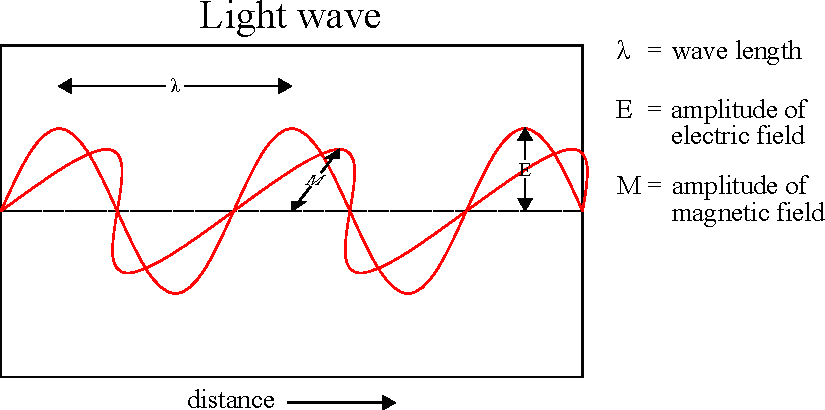
\includegraphics[width=0.6\linewidth]{Bilder/lightwave.pdf}
	\caption{Light as electromagnetic wave \tiny Gpvos 2007 wikipedia.org \ccbysa }
	\label{fig:LightasWave}
\end{figure}
 
 The polarization of light characterizes how the fields $\vec{E}$ and $\vec{M}$ orientation in space is distributed between different light waves. An unpolarized light source emits a chaotic orientated wave form. After polarized filtering only waves with the same orientation remain. The coherence of light describes correlations in the wavelength and the phase relation between the $\vec{E}$ and $\vec{M}$ oscillation. Coherent light sources cause interference between each other, resulting in a new coherent wave form. The coherence length is the distance of propagation where the wave is still of the same wavelength and phasing and can interfere with itself in the same way. Two interfering coherent waves in the same phase cause constructive interference. The amplitudes will sum up. A phase shift of $180^\circ$ between two coherent waves will result in a destructive interference and a subtraction of amplitudes. Incoherent waves that are polarized can still be monochromatic, meaning that the wave length is in a narrow band in the spectrum. However the phase and directions of the waves are randomly distributed between each other. 

\begin{figure}[!h]
	\centering
	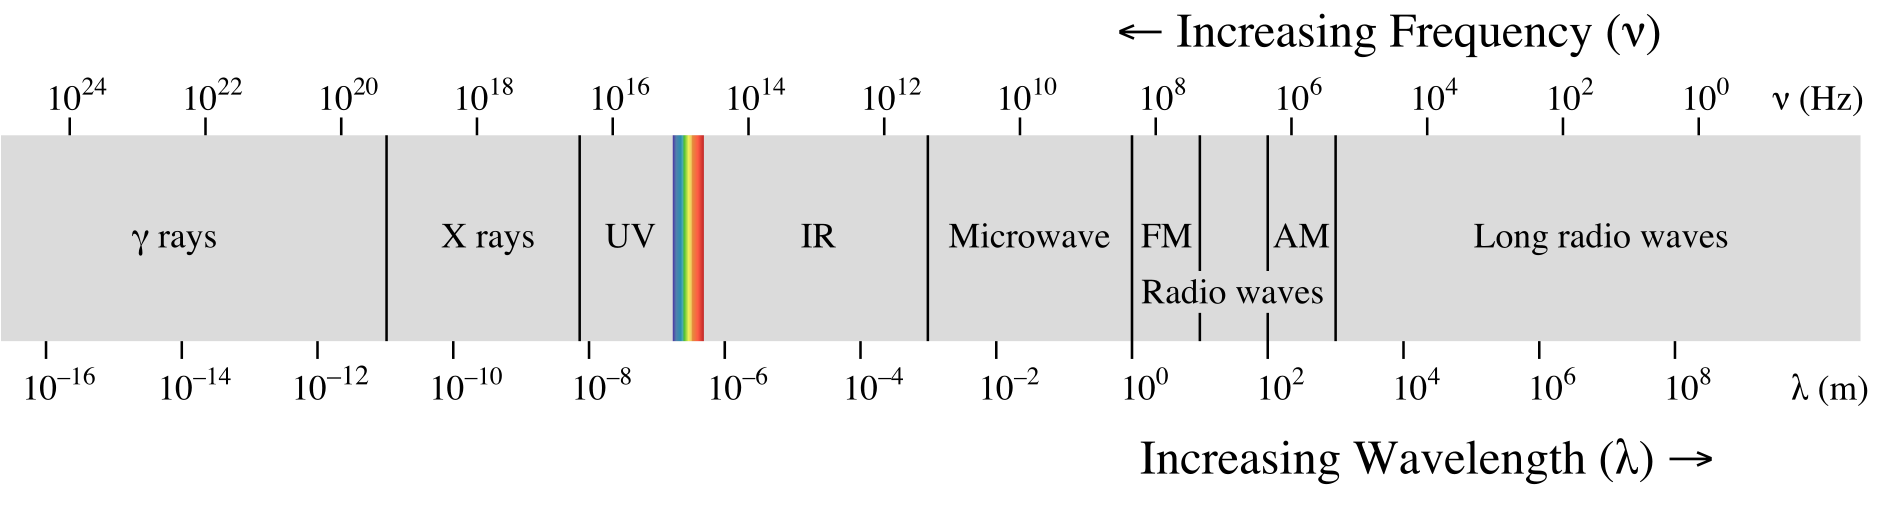
\includegraphics[width=0.7\linewidth]{Bilder/EM_spectrum.png}
	\caption{Electromagnetic spectrum \tiny Philip Ronan wikipedia.org \ccbysa}
	\label{fig:EM_spectrum}
\end{figure}

The Planck constant $h$ specifies the relation between energy E and frequency of light $\nu$. The radiant energy of one light beam can also be considered as a particle with the mass m, a so called photon.

\begin{equation}
 E =  h\cdot \nu=mc^2 ~~ [J]
\end{equation}

\begin{equation}
\lambda = \frac c \nu ~~[m]
\end{equation}
\medskip
 
 The mass-energy equivalence proves that light waves can be transformed into and from mass. This can be observed in the sun. The nuclear fusion of two hydrogen atoms results in a helium atom. A small amount of mass is lost in this reaction and transformed into electromagnetic energy that lightens our universe. The different wavelengths of a light source are represented in the electromagnetic spectrum. The sun's irradiance provides the complete electromagnetic power per square meter that is delivered on a surface in a certain distance. This value is corrected by the wavelengths of the specific light spectrum in the spectral irradiance. Figure \ref{fig:SolarSpectrum} shows the VIS and IR components of the sunlight and how they are influenced by the atmosphere of the earth in the spectral irradiance versus the wavelength.
 
\begin{figure}[!h]
	\centering
	\includegraphics[width=0.5\linewidth]{Bilder/Solar_spectrum.png}
	\caption{Solar radiation spectrum on earth \tiny Nick84 wikipedia.org 2013 \ccbysa}
	\label{fig:SolarSpectrum}
\end{figure}

The atmosphere of the earth absorbs various wavelengths that are related to the gas composition. Water ($H_2O$) and carbon dioxide ($CO_2$) absorb the infrared light of the solar spectrum while ozone ($O_3$) absorbs the high energy UV radiation. Nitrogen ($N_2$), however, is transparent for most components of the sunlight.


\subsection{Photometric and Radiometric Quantities}

Photometric (index v) and radiometric (index e) quantities are used for the quantification of light sources and lighting conditions. The human spectral sensitivity for visible light is considered in the luminosity function. The eye is capable to adapt its spectral sensitivity to different light conditions. Figure \ref{fig:luminosity} shows the CIE standard luminosity function V($\lambda$) in the photopic view under well-lit lighting and the scotopic view under low light. The peak of the photopic sensitivity can be found at about 555 nm which is the base for the normalization of the curve. The CIE luminosity function is a standard established by the Commission International de l'Eclairage and forms the central color matching function for light sources. The radiometric quantities consider the complete electromagnetic spectrum and are independent of the sensitivity of the human eye \cite{mccluney1994introduction}.

\begin{figure}[!h]
	\centering
	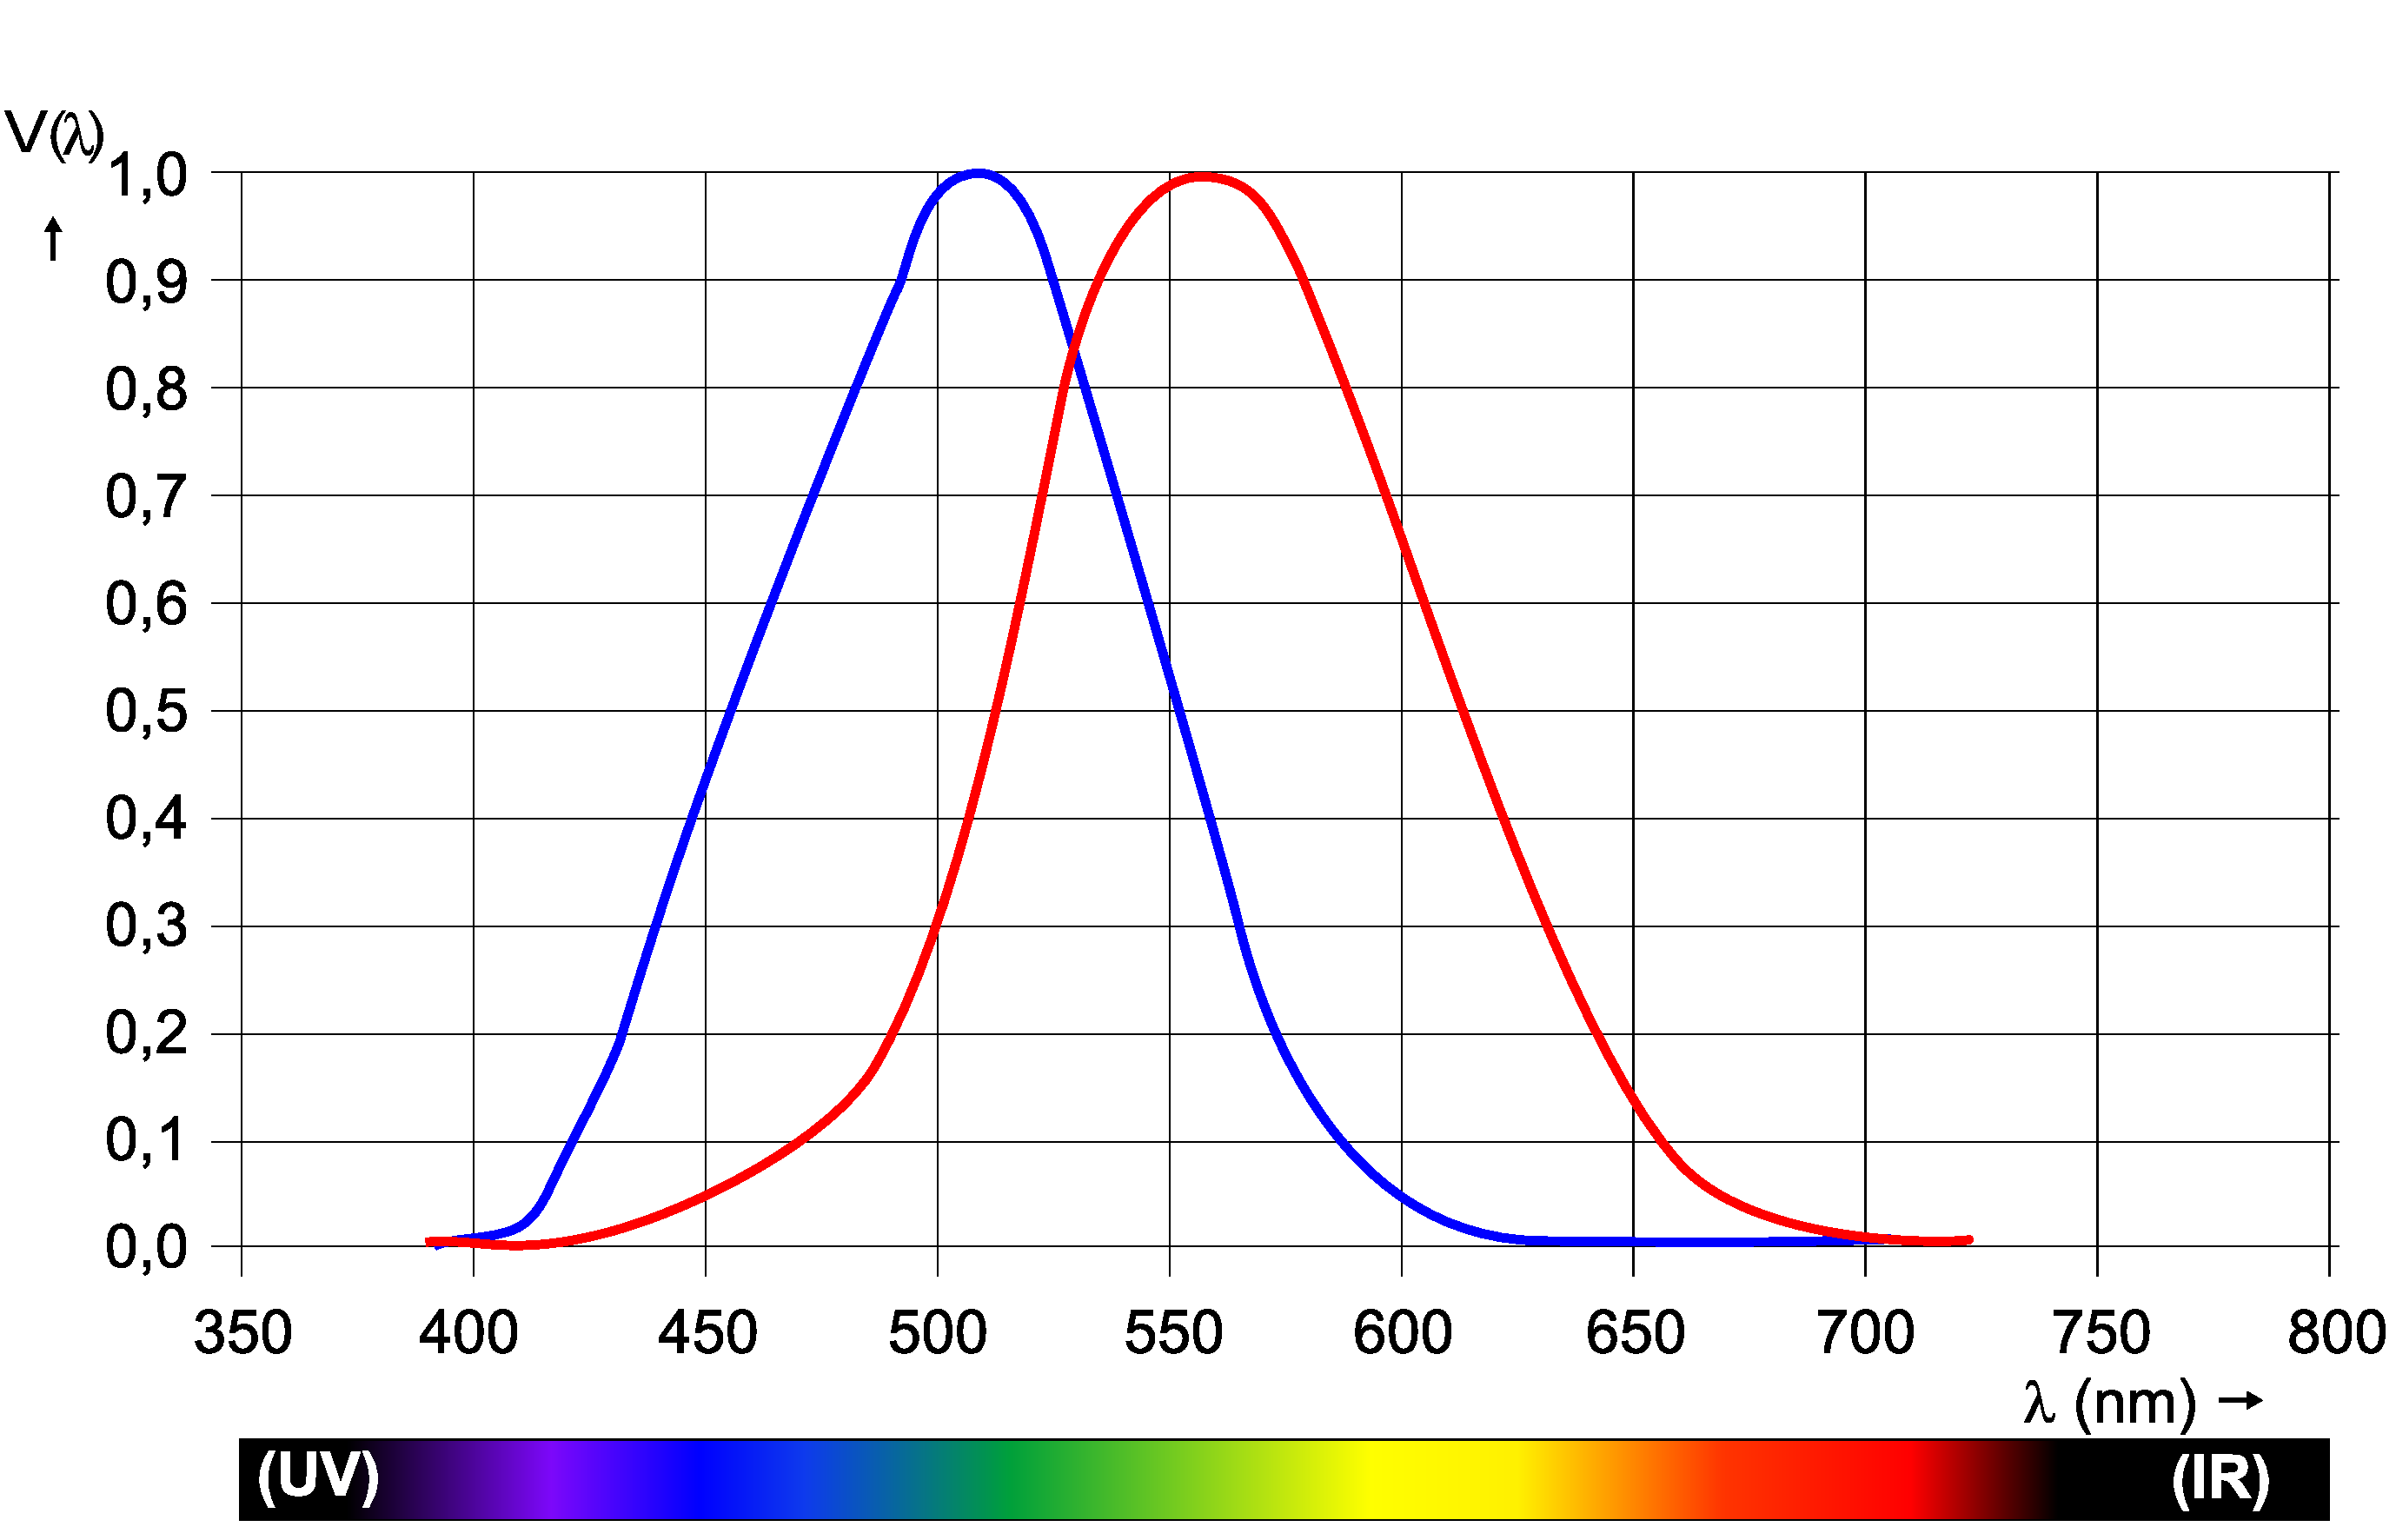
\includegraphics[width=0.5\linewidth]{Bilder/LuminosityCurve1.pdf}
	\caption{CIE Luminosity function V($\lambda$) of the human eye under low light (blue curve) and high light (red curve) conditions \tiny HHahn wikipedia.org \ccbysa}
	\label{fig:luminosity}
\end{figure} 

\subsubsection{Radiant and Luminous flux}

The radiant flux $\Phi_e$ is a scale for the radiant energy Q emitted per time unit on a surface. It is calculated by a given radiant intensity $I_e$ and the solid angle $\Omega$. In other contexts it is also called electromagnetic power: 

\begin{equation}
\Phi_e = \frac {dQ}{dt} = I_e \cdot \Omega ~~ [W]
\end{equation}
\medskip

The complement is called luminous flux $\Phi_v$ in the visible spectrum, with the unit\linebreak lumen [lm]. A light source with 1 cd, that emits in every direction in a solid angle of $4\pi$, will produce a luminous flux of $12.6~lm$. Every material above 0 kelvin radiates light, depending on the surface temperature. The radiated power can be calculated for a ideal black body that absorbs all radiation with the Stefan-Boltzmann-Constant $\sigma$, the material temperature T in kelvin, the emitting area A and the emissivity $\epsilon$ of the surface.

\begin{equation}
\Phi_e = \varepsilon(T)\cdot \sigma \cdot A \cdot T^4  ~~ [W]
\end{equation} 


\subsubsection{Radiant and Luminous Intensity}
 The radiant intensity $I_e$ is used for quantization of the total electromagnetic power emitted by a light source. The power is distributed on sphere areas while moving through space. One steradian (sr) defines an reference area $A=r^2$ on a sphere with the radius r. Figure \ref{fig:steradian} shows the propagation of light under the solid angle $\Omega$.

\begin{equation}
\Omega =\frac {A}{r^2}~~[sr^{-1}]
\label{eq:solid_angles}
\end{equation}

\begin{equation}
I_e=\frac {\Phi_e} {\Omega} ~~ [W sr^{-1}]
\end{equation}
\medskip
\begin{figure}[!h]
	\centering
	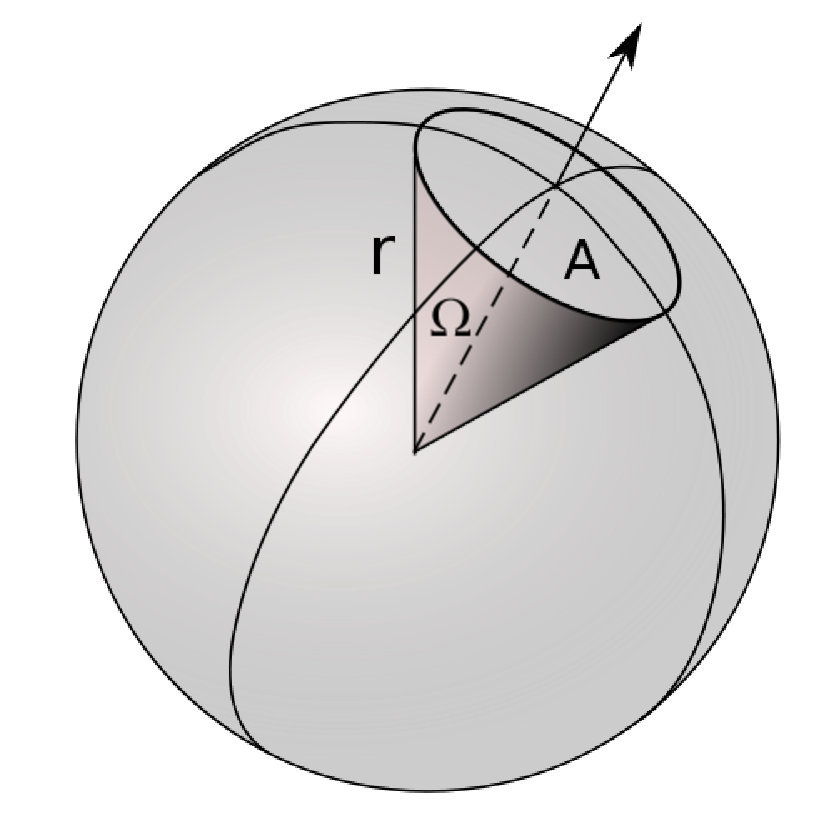
\includegraphics[width=0.3\linewidth]{Bilder/500px-Angle_solide_coordonnees.pdf}
	\caption{Propagation of light in one steradian \tiny Haade wikipedia.org \ccbysa}
	\label{fig:steradian}
\end{figure} 


The radiant power of visible light can be judged by the luminous intensity $I_v$. The power of the spectrum is adapted to the sensitivity of the human eye for different colors. The result is the wavelength-weighted power emitted by the light source per unit solid angle. The unit of luminous intensity is the candela (cd), an SI base unit:

\begin{quote}
	One candela is the luminous intensity, in a given direction, of a source that emits monochromatic radiation of a wavelength of 555 nm and that has a radiant intensity in that direction of $1/683$ watt per steradian\cite{taylor1999nist}.
\end{quote}

A 100 W light bulb offers a luminous intensity of about 1.1 cd. Modern LEDs in contrast can have up to 5 cd, due to the concentration of the emitted light in one direction and a higher luminous efficacy $\eta$ of up to 208 $lm W^{-1}$.

\subsubsection{Luminous Efficacy}
The amount of power P that is transformed in a light source into visible light is represented by the luminous efficacy $\eta_v$. The remaining energy will be radiated in other invisible wavelengths or transferred into a heat flow that vanishes into ambient material and air. 

\begin{equation}
\eta_v = \frac {\Phi_v}{P}
\end{equation}
\medskip

\subsubsection{Radiance and Luminance}
The radiance defined in equation \ref{eq:Radiance_and_Luminance_on_a_surface} is a measure for the quantity of radiation that passes through an area. It can also be used to quantify the amount of radiation, which is reflected from a surface in a specific direction. It changes with the cosine of the incident angle $\varphi$ normal to the emitting surface area. This equation is also called Lambert's cosine law and applies to diffuse reflecting surfaces or Lambertian surfaces.

\begin{equation}
L_e = \frac{I_e}{A_e} = \frac{d^2\Phi_v}{dA~d\Omega~cos\varphi} ~~ [W m^2 sr^{-1}]
\label{eq:Radiance_and_Luminance_on_a_surface}
\end{equation}

\begin{figure}[!h]
	\centering
	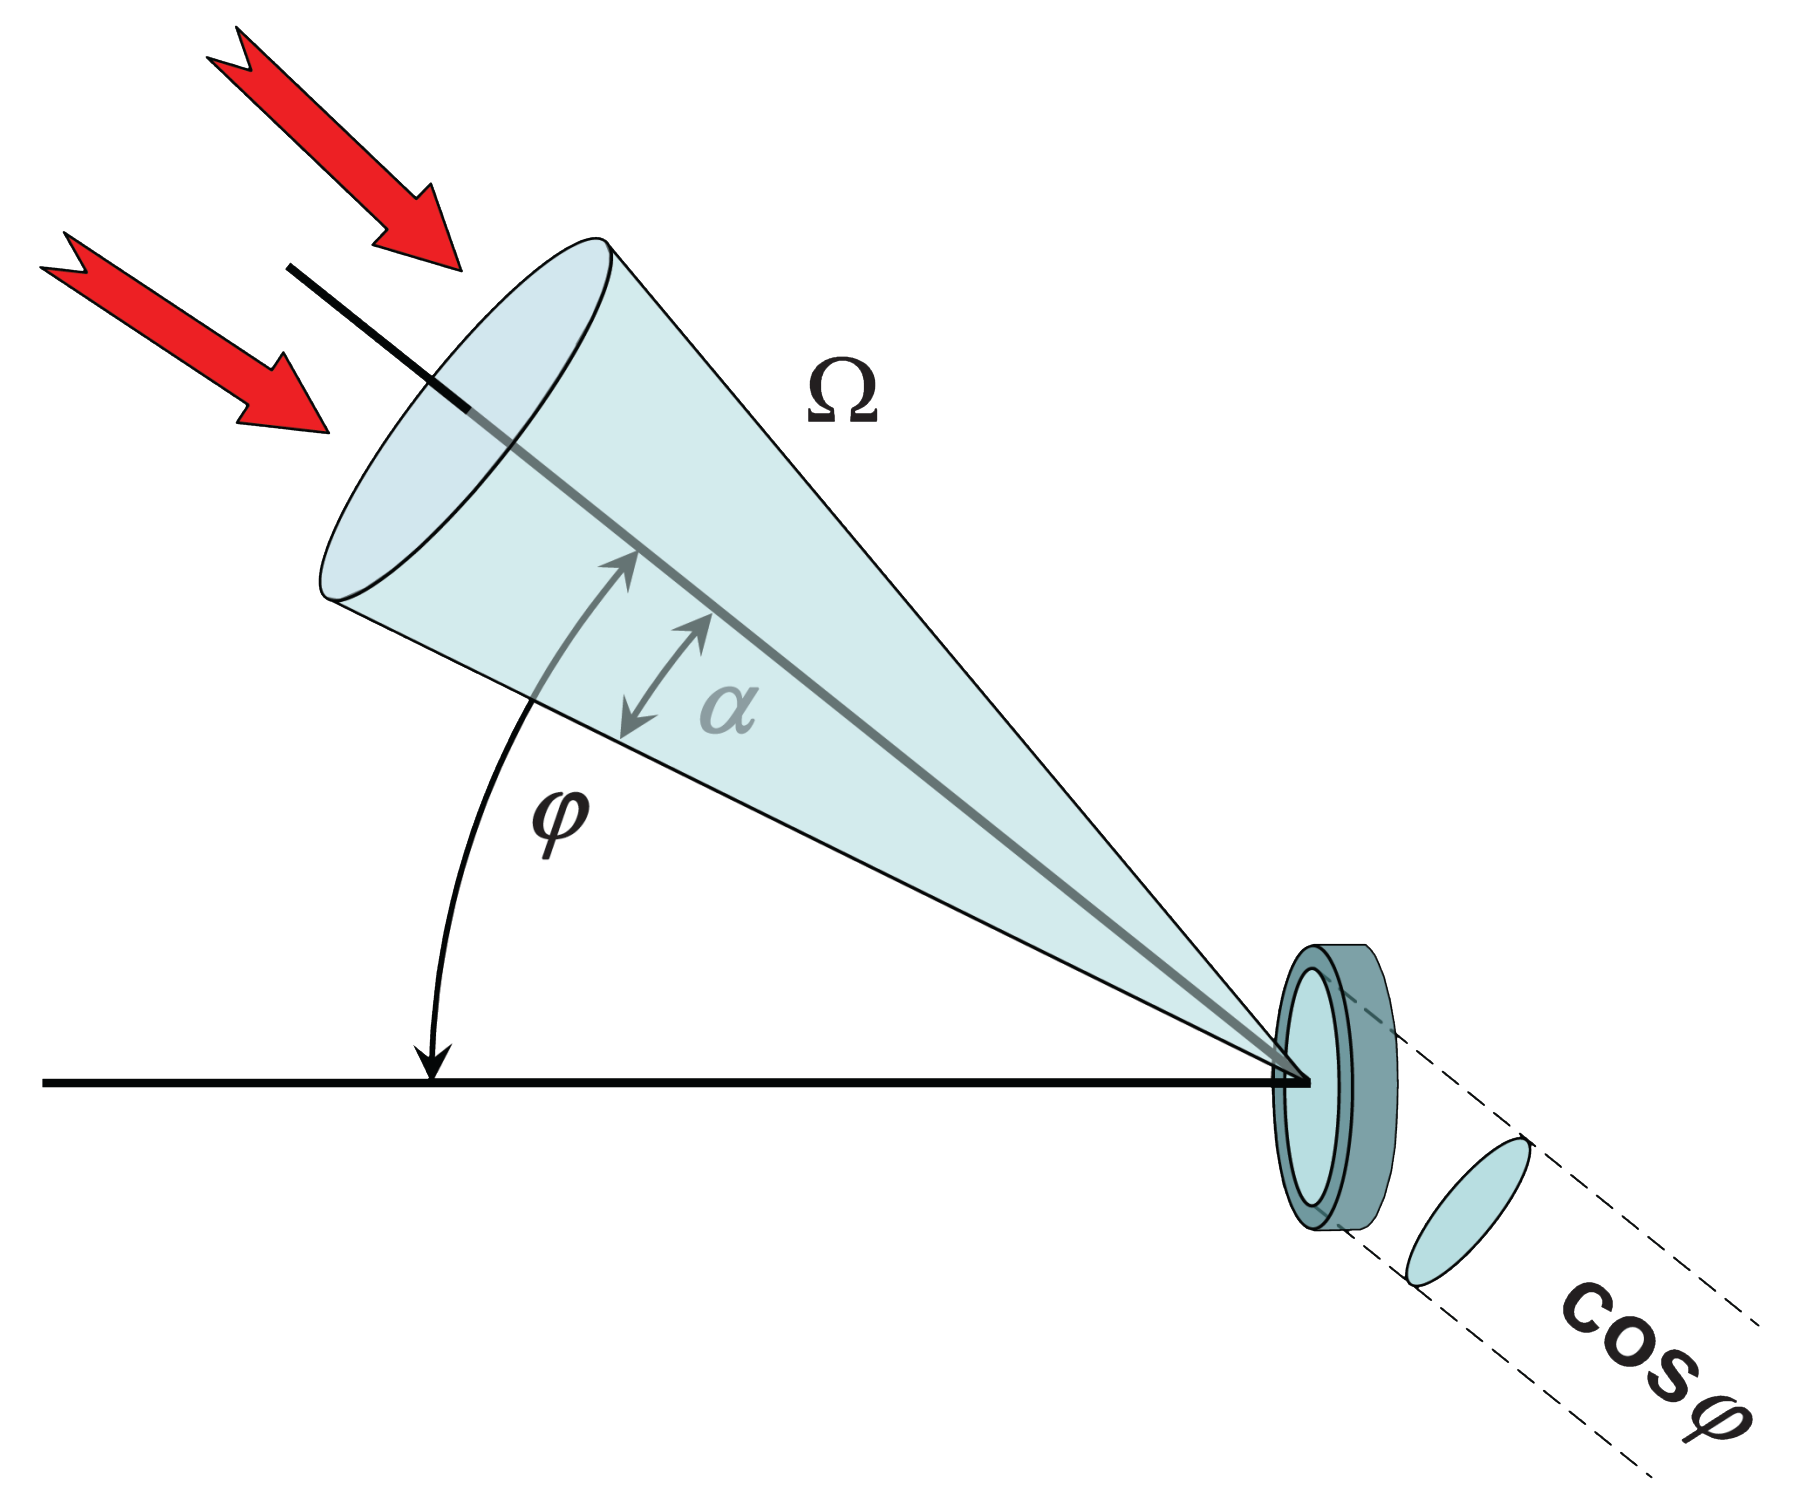
\includegraphics[width=0.4\linewidth]{Bilder/radiance.png}
	\caption{Radiance and Luminance on a surface}
	\label{fig:Radiance_and_Luminance_on_a_surface}
\end{figure} 

The luminance $L_v$ is the analog quantity with respect to the eye. It is a surface's grade of brightness to the human eye.

\subsubsection{Transformation from Radiometric into Photometric}

The radiometric quantities can be transformed into photometric quantities with the help of the Luminosity function V($\lambda$) and the efficacy of radiation $\eta_e$. With a radiant flux given in watt, this value can be compared with photometric quantities in lumen. Even if a light source emits low luminous flux, the destructive impact on the human eye can still be significant from the IR or UV spectrum. That is why for the hazard consideration, the radiometric quantities with specific wave lengths have to be considered. 

\begin{equation}
\Phi_v =\eta_e \cdot V(\lambda) \cdot \Phi_e ~~ [W] 
\end{equation}

\subsection{Diffuse, Spread and Spectral Reflection}

Depending on the wavelength, light interacts differently with material. The surface structure and material properties play a further role in the reflection and absorption characteristics. An ideal spectral reflecting area will radiate all light backwards with the same angle mirrored on the normal vector of the surface. Most materials can give specular reflection, provided that the surface is polished to eliminate irregularities within the magnitude of the wavelength. Transmission is the passage of the electromagnetic waves through a medium. The exit angle of the beam depends on the entry angle and the properties of the medium and light. Diffuse reflection is a combination between transmission and spectral reflection. The waves enter the material and are reflected on the surface multiple times before leaving it again. The direction of reflection is independent from the angle of the incident light. Ideal matt surfaces like white paper have this property and follow the Lambert's cosine law from equation \ref{eq:Radiance_and_Luminance_on_a_surface}. The mixture of diffuse and spectral reflection is called spread reflection and can be observed on most common material. In this case, a diffuse propagation will take place around the direction of ideal spectral reflection, depending on the incident angle \cite{hecht1987optik}. Figure \ref{fig:Diffuse_Reflection} shows the ideal diffuse, spread and spectral reflection of an incident light ray. The reflectivity is the fraction of the reflective $\phi_r$ electromagnetic power to the incident electromagnetic power $\phi_i$.

\begin{equation}
\varrho=\frac{\phi_r}{\phi_i}
\end{equation}

\medskip
 The transformation of radiation in other forms of energy in a medium is called absorption. Heat and other atomic reactions are created by the radiation interacting with the atoms. Some fluorescent materials, like phosphorous, emit the energy over a longer timespan in shifted wave lengths. The ratio of reflectance $\varrho$, transmittance $\tau$ and the absorption $\alpha$ must correspond to the conservation of energy. As a conclusion, equation \ref{eq:Optical_Energy_Convervation} must be fulfilled.

\begin{figure}[!h]
	\centering
	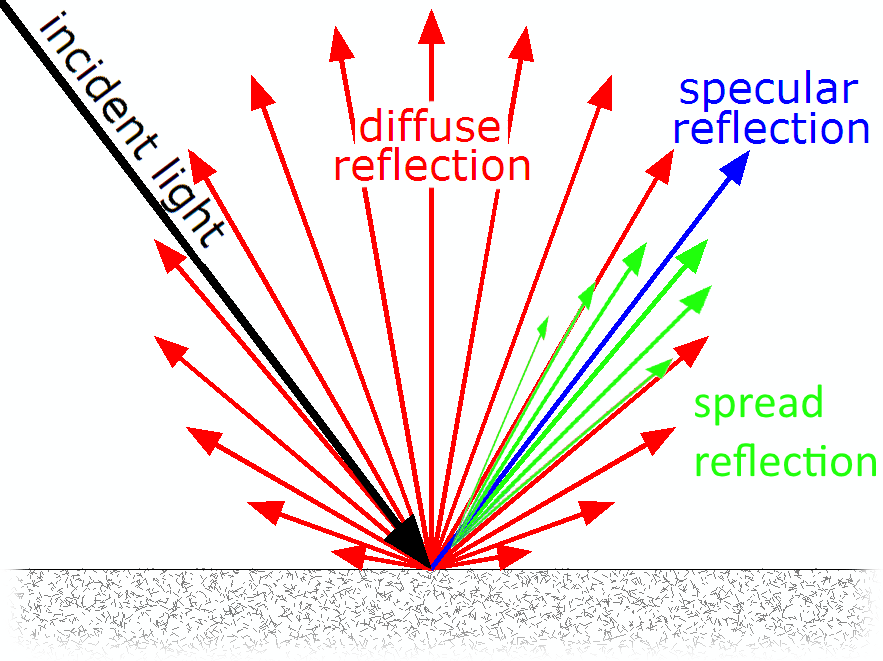
\includegraphics[width=0.4\textwidth]{Bilder/Diffuse_and_Spectral_Reflection.png}
	\caption{Reflection on an ideal mirroring surface and a diffuse surface \tiny GianniG46 wikipedia.org \ccbysa }
	\label{fig:Diffuse_Reflection}
\end{figure} 

\begin{equation}
\varrho +\tau + \alpha=1
\label{eq:Optical_Energy_Convervation}
\end{equation} 
\medskip

The reflectivity depends on the wavelength, the surface structure and the material. Infrared light is reflected in another way than visible light. White paper, for example, is a highly reflecting material for IR light with a reflectance of about $80~\%$. Black paper, in contrast, will absorb most of the incident light. In the reflectance spectrum, the reflectivity is plotted as a function of the wavelength. Aluminum reflects most of the incident light in the IR and VIS spectrum. Gold absorbs most of the radiation in the UV region and becomes reflective for red and IR wavelengths. Figure \ref{fig:Reflection on different metals} shows the reflection versus the wavelength for different metals.

\begin{figure}[!h]
	\centering
	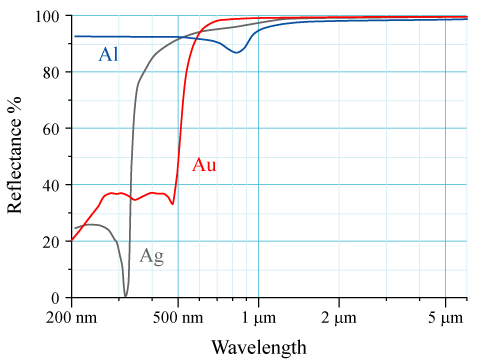
\includegraphics[width=0.5\linewidth]{Bilder/Image-Metal-reflectance.png}
	\caption{Reflectance spectrum of aluminium (Al), silver (Ag) and gold (Au) \tiny Bob Mellish wikipedia.org 2005 }
	\label{fig:Reflection on different metals}
\end{figure} 

\newpage
 
\subsection{Semiconductor Light Sources and Sinks}
 
Nowadays, light generation in semiconductor material plays a crucial role in all regions of illumination. Diodes consist of a chip of two layers of semi-conducting material, which are doped with impurities. As in most diodes, current flows from the anode to the cathode when a threshold voltage $U_{th}$ is reached between both layers. The anode consists of negatively charged holes (p) and the cathode delivers positive charges (n) in form of electrons. The contact area between both materials is called space charge region or depletion area. It gets conductive when the threshold voltage is reached. A current flow in the reverse direction is not possible under normal conditions. Figure \ref{fig:Pnjunction} shows the distribution of impurities in a common diode.
\begin{figure} [!h]
	\centering
	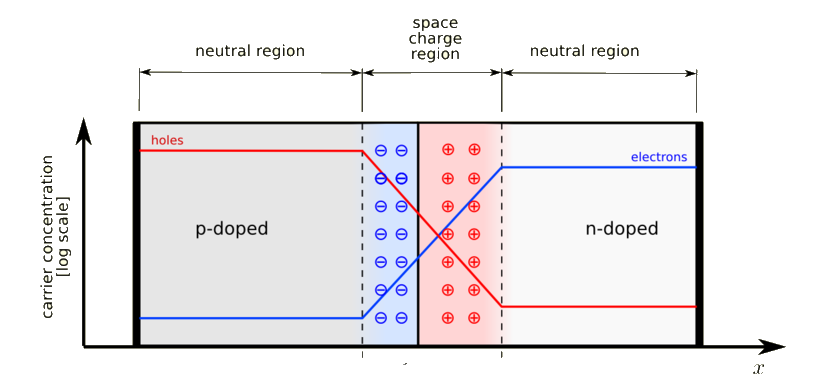
\includegraphics[width=0.6\linewidth]{Bilder/Pn-junction-equilibrium.png}
	\caption{p-n junction of a diode \tiny TheNoise wikipedia.org \ccbysa}
	\label{fig:Pnjunction}
\end{figure}

The recombination of the charges releases energy in the form of radiation. The energy difference between the top of the valence band (holes) and the bottom of the conduction band (electrons) is described by the band gap. The emitted wavelength depends on the size of the gab and the corresponding voltage that drops in this region. For infrared LEDs gallium arsenide (GaAs) or aluminium gallium arsenide (AlGaAs) are used as semi-conducting materials. The emitted wavelength depends on the voltage drop and on the semiconductor material.

A current will flow through a GaAs IR diode at a voltage higher than $1.63~V$. Blue light is emitted from indium gallium nitride diodes and a $U_{th}$ higher than $2.48~V$. This process does also work in the opposite direction. Incident radiation with a wavelength according to the band gap of the diode induces a voltage. In general, this process is possible in every diode, but photo diodes are very sensitive to incident light. That is why this components are used to measure radiation. Figure \ref{fig:thresholdvoltage} shows the current curve versus voltage of an silicon diode. $U_{th}$ is defined as the point with a current flow of $1~mA$. Higher radiant intensity can be achieved through an increase in voltage, which causes a higher current flow \cite{tschirleyelektronik}. With a decreasing temperature, the threshold voltage $U_{th}$ will be shifted to higher values.\\


\begin{figure} [!h]
	\centering
	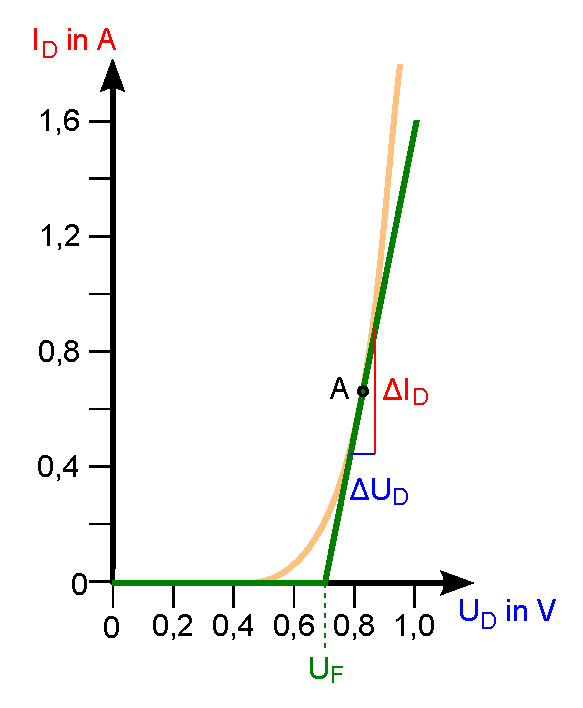
\includegraphics[width=0.4\linewidth]{Bilder/Dioden-Kennlinie_1N4001_differentiell.pdf}
	\caption{Diode current versus voltage \tiny Stuendle 2011 wikipedia.org}
	\label{fig:thresholdvoltage}
\end{figure}

\subsubsection{Light-Emitting Diodes}

With the development of blue LEDs in 1994 new ways of lightning were possible. Other colors, such as red, were discovered in 1968, but only with the discovery of the color blue, the total visible spectrum was covered. The high efficiency and the long lifetime of LEDs offer huge steps in illumination in comparison to light bulbs or halogen bulbs. For the human sensation of white light, another problem had to be solved with LEDs. The color rendering index (CRI) is a measure how the LED reveals the color of illuminated objects in reference to the sunlight. The little fraction of red light in the white spectrum modifies the color of illuminated objects. The light seams to be "cold". More red light on the other hand reduces the luminous efficacy, but increases the CRI value.\\

The electromagnetic spectrum of a LED can be approximated by the Gaussian distribution. A blue LED will emit light with wavelengths between 450 and 500 nm. This range is called spectral width. The speed of respond is often given by the rise and fall time; the time required to go from  $10~\%$ to $90~\%$ power. The shortest possible pulse length with modern fast LEDs can be shorter than $1~ns$. As a conclusion results the maximum switching frequency can be up to multiple megahertz for LEDs.\\   
White light can be generated by the combination of red, green and blue. Another method is the coating of a blue LED with phosphor: A fraction of the blue light undergoes a wavelength shift, being transformed from shorter to longer wavelengths.\\

There are two basic types of LED structures: Edge emitters and surface emitters. Surface emitters have a comparatively simple structure. The light will be radiated in all directions from the surface of the semiconductor. The total optical output power is higher than the one from edge emitters. In contrast, edge emitters have a smaller spectral width, a very high power density and a internal optical gain like a laser. The light leaves the chip between the layers on the edge of the semiconductor \cite{botez1979comparison}.\\

The normalized radiant intensity as function of the angle of radiation can be determined experimentally and characterize from different angles. These diagrams are often published by manufacturers in the data sheets of the light source as shown in figure \ref{fig:radiation_diagram} for a common IR LED. \\

\begin{figure} [!h]
	\centering
	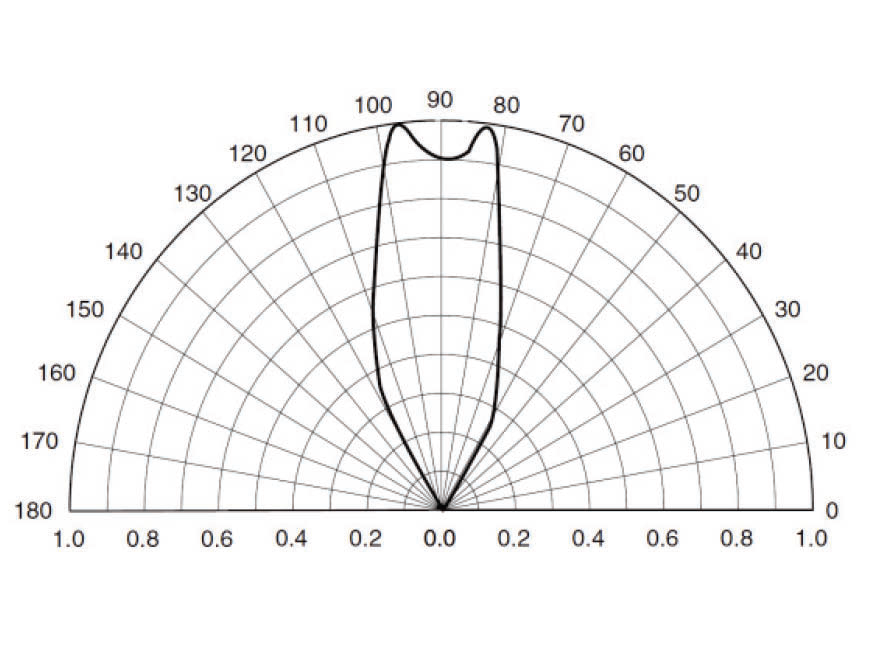
\includegraphics[width=0.5\linewidth]{Bilder/radiation_diagram.png}
	\caption{Radiation diagram of a IR LED \tiny QED222 www.fairchildsemi.com}
	\label{fig:radiation_diagram}
\end{figure}

\newpage

\subsubsection{Laser Diodes}
Laser diodes in contrast to LED create monochromatic light in a narrow bandwidth. An additional undoped intrinsic semiconductor is implemented between the p-n junction. It emits light waves with  chronologically steady polarization and phases to each other. Therefore, ideally only a fixed wavelength is created. As a conclusion the oscillation of the emitted light is therefore phase-synchronous. The beam deivergence is low. This property is called collimated in optics \cite{thompson1980physics}. An important advantage of laser diodes is the fact, that it can be modulated in intensity with high frequencies up to several gigahertz and extreme short pulses in the region down to femtoseconds. In most technical implementations, the laser light intensity will be additionally measured with a photo diode near the laser diode to get a feedback for precise control. Unlike a regular diode used in electronics, the goal for a laser diode is that all carriers recombine in the I region, and produce light. Thus, laser diodes are fabricated using direct bandgap semiconductors. Figure \ref{fig:laserdiode} illustrates the setup of a laser diode on its heat sink, the monitoring photo diode and the protecting window.

\begin{figure} [!h]
	\centering
	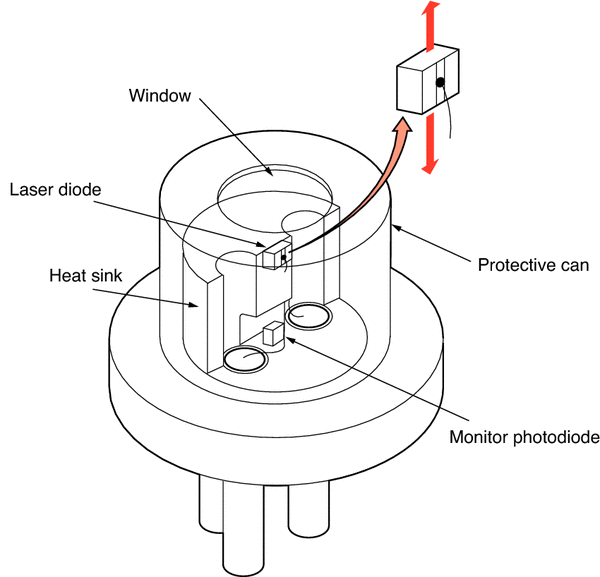
\includegraphics[width=0.5\linewidth]{Bilder/laser_diode.png}
	\caption{Setup of a common laser diode \cite{newport}}
	\label{fig:laserdiode}
\end{figure}

\subsubsection{Photo Diodes} 
Photo diodes are used for the conversion from radiant into electrical energy. The physical principle behind this is the inner photoelectric effect. If absorption of light occurs in the junction, holes move to the anode and electrons to the cathode. A current is induced and therefore a voltage can me measured. The responsivity $R_\lambda$, also known as responds, is the ratio between the current flow relative to the radiant power in different wavelengths. The quantum efficiency (Q.E.) is defined as the fraction of the incident photons, that contribute to photo current.

\begin{equation}
R_\lambda = \frac{I_P}{P} ~~ [A W^{-1}]
\end{equation}

\begin{equation}
Q.E. = R_\lambda \cdot \frac {h c} {\lambda q}~~[1]
\end{equation}

\begin{figure} [!h]
	\centering
	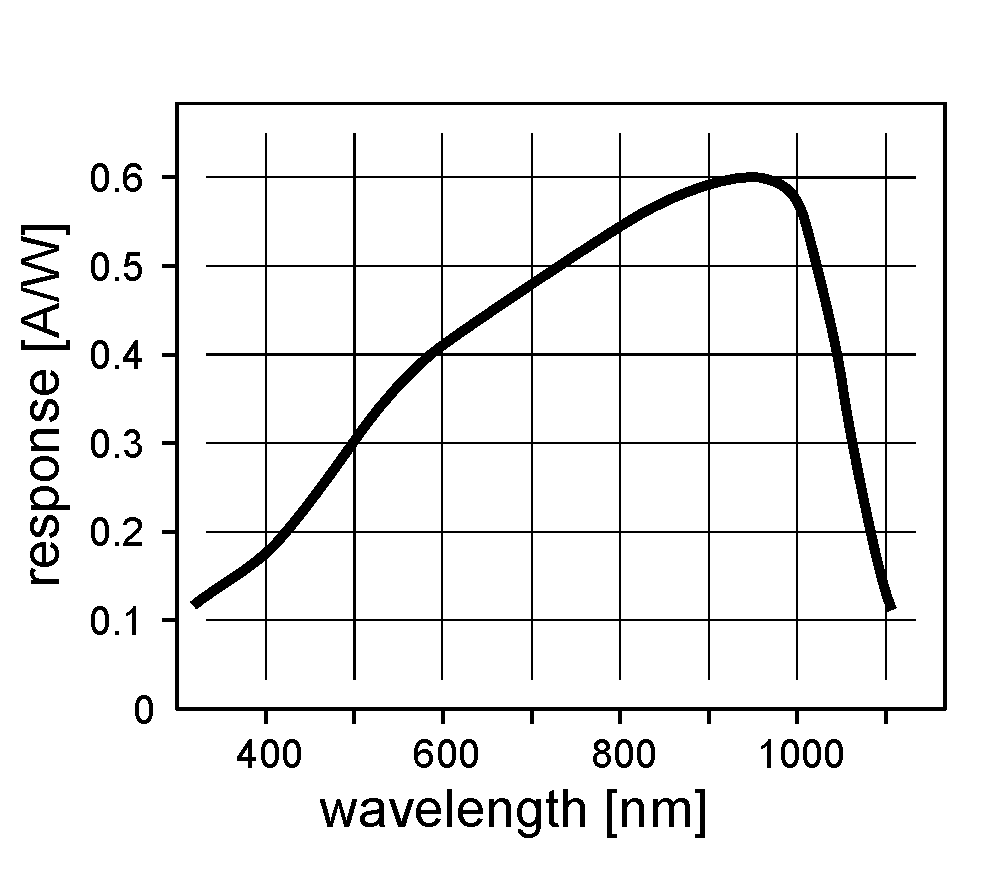
\includegraphics[width=0.5\linewidth]{Bilder/Response_silicon_photodiode.pdf}
	\caption{Response over wavelength of a silicon photodiode \tiny Kai Martin 2007 wikipedia.de \ccbysa}
	\label{fig:response}
\end{figure}

Every signal of the photo diode will be overlayed by dark current and thermal current. This noise results from electromagnetic background radiation and thermal movement of the charge carriers. To achieve the raw noise characteristics of a photo diode, the output signal must be measured in an absolute dark room with no background radiation. 

The rise and fall time of a photo diode can be expressed as the frequency response at which the output amplitude decreases by $3~dB$. Three factors influence the response time:
\medskip \\
\begin{enumerate}
\setlength\itemsep{0.001em}
\item The charge collecting time of the carriers in the depleted region. 
\item The charge collecting time in the undepleted region.
\item The resistance and capacity of the diode circuit combination.
\end{enumerate}

\begin{equation}
t_r \cong \frac{0.35}{f_{3dB}}~~[s]
\end{equation}
\medskip

Single-photon avalanche diodes (SPAD) are very sensitive to incident light and enable the measurement of very low intensities. The electric field between the junction is so high, that the arrival of a single photon can be determined down to ten picoseconds. A photo-generated carrier triggers an avalanche current due to the impact of ionization mechanism. The circuit behind the diode must fulfill multiple tasks \cite{cova1996avalanche}:

\begin{enumerate}
	\setlength\itemsep{0.001em}
	\item Sense the leading edge of the avalanche current. 
	\item Generate a standard output pulse synchronous with the avalanche build-up.
	\item Quench the avalanche by lowering the bias down to the breakdown voltage.
	\item Restore the photo diode to the operative level.
\end{enumerate}

\subsection{Image Sensors}
A radiant flux can be converted into a 2D data matrix by an image sensor, an array of photo diodes. Every single element of the array, a so-called pixel, consists of one or multiple photo diodes, that are arranged in columns and rows. The pixel pitch is the dimension of a single pixel. The area that is actually sensitive to the light is determined by the fill factor times the pixel pitch. Without a micro lense, this area corresponds to the photodiode surface. The physical extent of the complete flat sensor is called optical size. An ordinary picture of visible light consists of a mixtures of red, green and blue (RGB) colors, but single photo diodes can only be optimized for a narrow band in the light spectrum. The band gap must correspond to the wave length of the light to detect it. Therefore three diodes are needed to deliver the RGB information on one pixel. They can be arranged side by side or stacked. The classical Bayer filter separates the light with red, green and blue filters. Foveon X3 sensors, in contrast, use three stacked photo diodes with various band gaps. IR image sensors are made of special semiconductor material like Indium Gallium Arsenide. 

\subsubsection{Charged-Coupled Device Sensor}

The first digital image sensor was based on the charged-coupled device (CCD) architecture. In the first place Bell Labs invented this type of integrated circuit for data storage in shift register. Charges could be shifted between the different capacitors that hold the energy of each diode. Later, it was discovered that this circuit can also be used as an image sensor. After the array is exposed to light, every pixel contains information about the incident light in form of charges. This data is transferred into a storage pixels array. Gathered charges are transformed into a corresponding voltage by a single amplifier in series order. The signal can be converted afterwards into a digital representation or into a continuous analog signal. The bit depth or color depth of the analog-to-digital converter (ADC) is given in bits and specifies the number of possible steps for the discretization. The color precision depends on this value and on the amplifier characteristics.


\subsubsection{Complementary Metal-Oxide-Semiconductor Sensor}

Modern semiconductor technology lead to the development of image sensors that are produced based on complementary metal-oxide-semiconductors (CMOS), also called active-pixel sensor. In contrast to CCD, every pixel is implemented with his own amplifier. Other components, like the ADC or the oscillator are integrated onto the sensor chip. This allows production under a much lower cost. Thus most consumer market cameras nowadays are based on this technique. The simplest realization of an CMOS pixel can be done by a photo diode and three CMOS transistors as shown in figure \ref{fig:CMOS_architecture_storage_pixels}. The charges will be gained inside every pixel after the exposure time. The circuit can be discharged via the reset connection, for every new image.

\begin{figure} [!h]
	\centering
	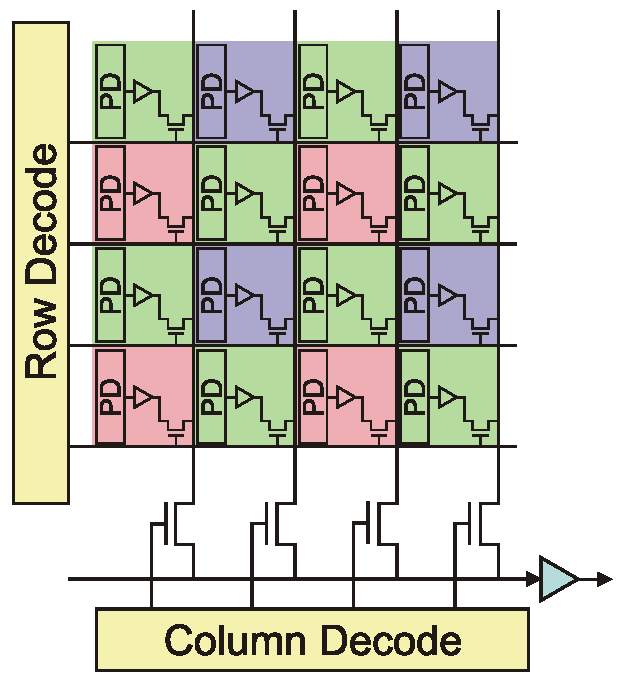
\includegraphics[width=0.4\linewidth]{Bilder/CMOS_Image_Sensor_Mechanism_Illustration.pdf}
	\caption{Frame transfer in a CMOS image sensor \tiny Shape 2008 wikipedia.de}
	\label{fig:CMOS_architecture_storage_pixels}
\end{figure} 

\newpage
\subsubsection{Attributes of Image Sensors}
For the foreseeable future, CCD and CMOS sensors will play both a significant role in imaging procedures. The long experience with CCD sensor production and the associated reliability is one of the major advantages in comparison to CMOS for scientific applications. Nevertheless, CMOS technology gains growing interests for scientific applications with developments driven by the consumer market. The following attributes are used to differ between the characteristics of both images sensors \cite{neugebauer1991parallel} \cite{litwiller2005cmos}.\\
     
\textbf{Dynamic Range}\\
The ratio between the saturation of a pixel to its threshold to detect photons is called the dynamic range (DNR). Saturation is reached when additional light will not cause more charges. The DNR is often represented in decibel. A low threshold is only possible with a low Signal-to-Noise Ratio (SNR). It describes the power ratio between the signal that needs to be measured and the unwanted background noise \cite{bushberg2011essential}. 

\begin{equation}
DNR = 20\cdot\log{\frac{P_{saturation}}{P_{threshold}}}
\end{equation}

\begin{equation}
SNR = \frac{P_{signal}}{P_{noise}}
\end{equation}
\medskip

The human eye has its highest dynamic range in the green spectrum. It enables us to see very small differences in color and brightness in this range. The contrast radio describes the same property for display systems. A high contrast radio is desired for most displays. Small shades between colors can be distinguished better.\\  

In the past CCDs enjoy significant noise advantages over CMOS because of less circuits on the chip that interfere the measurement. ADCs and other components are outsourced from the image sensor. This issue has been solved by the development of modern CMOS and the possibility to integrate the signal processing at the sides of image sensor, which has substantially dampened many noise sources and improved CMOS performance.\\ 

\textbf{Uniformity}\\
Ideally, every pixel should behave in the same way under identical illumination conditions. In practice, inaccuracies in the semiconductor production cause small variance in the structure of the photo diodes. This problem occurs with CCD and CMOS. CCDs benefit from the single amplifier, that every charge goes through. As a conclusion all values are increased with the same gain. In CMOS variations between the amplifier causes a higher uniformity. This is a significant issue in high-speed applications with a limited SNR. The short exposure time gathers only small amounts of charges. Consequently uniformity between the pixels will emerge under the short exposure time.\\   
  
\textbf{Speed}\\
The highly integrated CMOS technology makes this type of sensor much faster than CCD. Capacitance and propagation delays are shorter, because the circuitry is integrated into the chip. The charge transfer time is much shorter and the ADC processing can be done directly in the image sensor. This results in much higher speeds with CMOS. Images can be made in a very short distance to each other. Therefore, CMOS allows higher frames-per-second (fps). \\

\textbf{Windowing}\\
One limitation for the maximum speed of a camera is the ability to transfer and save all captured images. CMOS sensors allow the independent operation of parts on the image sensor. The number of working pixels is decreased to increase the maximum possible speed between every capture. This function is called region-of-interest (ROI) or windowing in modern industrial cameras.\\

\textbf{Antiblooming}\\
Blooming is the unwanted movement from charges between pixel in saturation. CMOS is immune for this effect, because every pixel is separated from each other. Modern CCD reduce this effect with the help of Anti-Blooming Gates. Unfortunately, this limits the size of the pixel and therefore the dynamic range.  

\subsubsection{Rolling and Global Shutter}
In traditional analog photo cameras, the shutter speed is the time in which the film is exposed to the light. The shutter opens and closes mechanically. The time in between is also called exposure time $t_e$. Today this is done without any mechanic in a digital camera. The sensor starts, stops and resets based on a digital control signal. Two different types of electronic shutters can be distinguished. The rolling shutter is used in most CMOS consumer cameras. The rows of the image sensor start their measurement shifted to each other. This causes the rolling shutter effect when fast moving scenes are measured in the order of the exposure time or smaller. The time delay between the lines can produce a blur in the picture. This kind of shutter is not desired for scientific and industrial investigations of fast moving objects. Figure \ref{fig:Rolling_shutter} shows the timing of a rolling shutter image sensor. 

 The global shutter is used in most scientific and industrial cameras. Every row of the image is exposed at the same time without any phase shifting. In the past, this was one of the main benefits of CCD cameras. New developments allow the combination between global shutter and CMOS. Figure \ref{fig:Global_shutter} shows the timing of a CMOS global shutter camera. Images can be captured without geometric distortions. A longer readout time is necessary for the processing of charges in parallel. The camera is "blind" in this time slot for incident light. A flashlight synchronized to the camera trigger is a indicator that is commonly used to investigate the shutter of the camera. A trigger input or output at the camera allows the synchronization of the image exposure to the flash or other devices. The camera and the lighting can be shifted to each other to evaluate the timing of the reset, exposure, readout and charge transfer. For the synchronization between multiple cameras, the trigger channel enables the fixed phase relation between images from different perspectives. This is especially necessary when dynamic processes are investigated. The exposure time $t_e$ must always be smaller than the frame periode. Consequently, the exposure time must be reduced with higher frame rates (fps):
 
 \begin{equation}
 t_e < \frac{1}{fps}
 \end{equation}
 \medskip

\begin{figure} [!h]
	\centering
	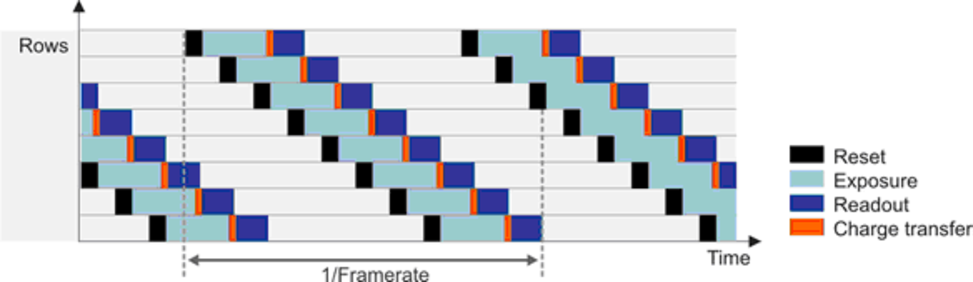
\includegraphics[width=0.6\linewidth]{Bilder/rollingshutter.pdf}
	\caption{Timing of rolling shutter CMOS Sensor \tiny http://www.cihansari.com/}
	\label{fig:Rolling_shutter}
\end{figure} 

\begin{figure} [!h]
	\centering
	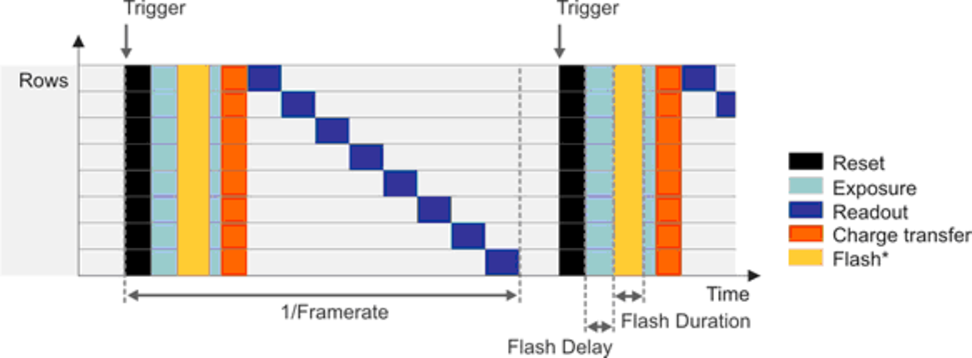
\includegraphics[width=0.6\linewidth]{Bilder/globalshutter.pdf}
	\caption{Timing of triggered global shutter CMOS sensor \tiny http://www.cihansari.com/}
	\label{fig:Global_shutter}
\end{figure}  

\subsubsection{Camera Optic} 
The image sensor without a lens in front of it is not able to capture a sharp image. The ambient light from different angles will overlap on multiple pixels. That is why a lens is needed to direct the path of the light rays as parallel as possible on the sensor. Every point of the scene should ideally be represented on the image sensor only on one position. For different distances this is not possible with a fixed lens position. A focus is needed to change the plane of the lens and therefore the focal length $F$. As a consequence the plane in which the scene is captured sharply is moved. Figure \ref{fig:focal_length} shows some basic dimensions of the camera optic. With a higher maximum $F$, sharp pictures can be made from a long distance $d$. The angle of view $\theta$ is reduced in contrast. The focal length is a scale for the optical power of a lens and to measure how strong the rays are bended. The optical axis stands normal to the middle of the image plane and point into the middle of the investigated scene. 
\begin{figure} [!h]
	\centering
	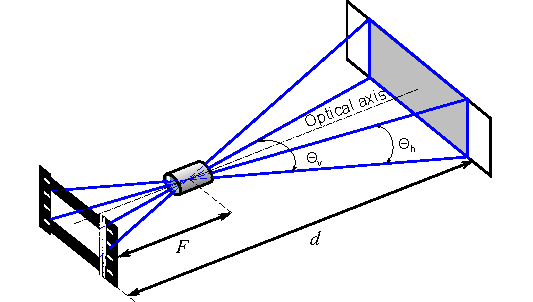
\includegraphics[width=0.5\linewidth]{Bilder/angle_of_view_3d.pdf}
	\caption{Focal length in the camera optic \tiny Christophe Dang Ngoc Chan 2007 wikipedia.org \ccbysa}
	\label{fig:focal_length}
\end{figure}  

The field of view (FOV) is the image section of the scene that is observed. In an optical instrument it describes the solid angle through which a detector is sensitive to incident electromagnetic radiation. The aspect ratio of the resulting images corresponds to the aspect ratio of the field of view. It can be calculated by the vertical and horizontal angle of view $\theta_{v,h}$, as described by equation \ref{eq:aspect_ratio}.

\begin{equation}
\label{eq:aspect_ratio}
Aspect~Ratio = \frac{\tan({\theta_v})}{\tan({\theta_h})}
\end{equation}

 The lens speed N is the ratio between the maximum possible aperture and the focal length of the objective. The illuminance, that can be captured by the lens, increases with the square of the aperture. A lens with a larger maximum aperture is called a fast lens because it delivers more light in the same exposure time.
 
\begin{equation}
N=\frac{F}{D}
\end{equation}

\subsubsection{Motion Blur}
Motion blur occurs when the sensor or an object in the scene moves within the exposure time of an image. One observed point will be projected to multiple positions on the image sensor. This can be avoided with a very short exposure time $t_e$ or with a stroboscope in a dark room that controls the amount of light in the scene. The movement $\vec{s}_{blur}$ of every point inside a picture can easily be calculated when the velocity $\vec{v_p}$ parallel to the picture plane is known and constant.

\begin{equation}
{\vec{s}_{blur}} = \vec{v_p}\cdot t_e ~~[m]
\label{eq:motion_blur}
\end{equation}

Figure \ref{fig:motionblur} shows the motion blue on a propeller. The speed on every point on the blades $\vec{v}$ can be calculated with angular velocity $\vec{\omega}$ and the radius $\vec{r}$ to the axis of rotation. The velocity $\vec{v_p}$ is the projection of $\vec{v}$ on the image plane. The blur increases linear with the radius to the axis.

\begin{equation}
\vec{v} = \frac{d\vec{r}(t)}{dt} = \vec{\omega}\times \vec{r}~~[ms^{-1}]
\end{equation}

The scalar angular velocity can be calculated by the rotational speed n. With the axis of rotation as z the vectorial angular velocity can be derived. This can also be used to calculate the rotational speed from a blurred picture with known exposure time and geometry of the rotor. 


\begin{figure} [!h]
	\centering
	\fbox{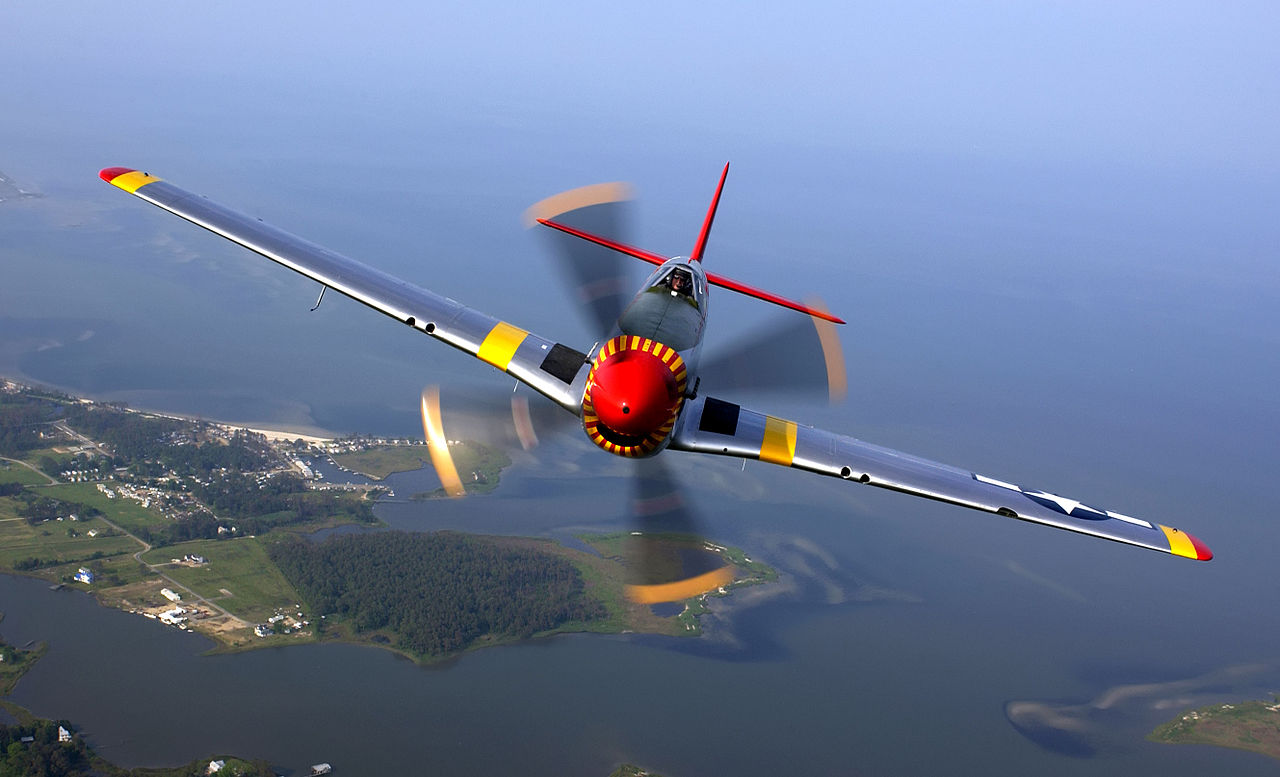
\includegraphics[width=0.45\linewidth]{Bilder/P-51_Mustang_edit1.jpg}}
	\caption{Motion blur of a fast moving rotor \tiny Tech. Sgt. Ben Bloker wikipedia.org}
	\label{fig:motionblur}
\end{figure} 

\newpage

\subsection{Range Imaging Techniques}
Multiple 3D scanning approaches are used, to derive three-dimensional data from the real world. In this section, a comparison of different range imaging techniques and their characteristics is done. They all produce 2D images, that represents the distance to every point in the scene, a so called range or depth image. This data can be transformed into a 3D space, when the system is calibrated adequately to the field of view, which depends on the focal length or freedom of movement of the laser. Various methods have been developed, to determine the distance to the image sensor.


\subsubsection{Stereo Triangulation}
The position of a point in space can be reconstructed from the perspective of two or more cameras. This requires a calibrated position and field of view of the cameras to each other. With two images of the same scene, taken from different points of view, the correspondence problem has to be solved. It describes the challenge of finding a set of points in one image, which can be identified as the same points in the other image from a different point of view. Two basic methods are distinguished:\\

\textbf{Correlation-based} - Check if identical location can be found in both images.\\
\medskip
\textbf{Feature-based} - Find multiple features in the images and see if a layout of subsets is similar.\\

\begin{figure} [!h]
	\centering
	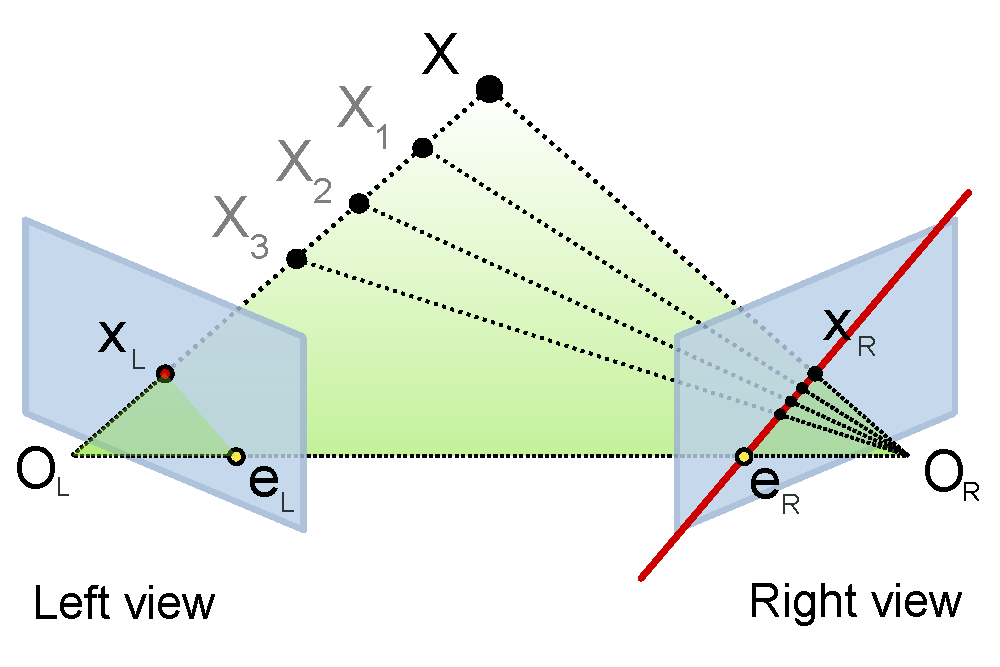
\includegraphics[width=0.6\linewidth]{Bilder/Epipolar_geometry.pdf}
	\caption{Basic principles of stereo triangulation \tiny Arne Nordmann 2007 \ccbysa }
	\label{fig:stereovision}
\end{figure} 

Markers are easy additives to identify single points from multiple perspectives. Figure \ref{fig:stereovision} shows one scene that is observed from two position. The point $X$ is projected as $X_R$ and $X_L$ on both image sensors. The epipolar line between $O_L$ and $O_R$ is the base for the triangulation \cite{finsterwalder1897geometrischen}. The position of the point X cannot be distinguished in the depth with just the left image. With the second image, the range of every point can be calculated. The nearer the objects are to the image sensor, the higher  the displacement of the object between the two images is. Therefore, the triangulation is simplified and more accurate. The human eyes work by the same principle to determine the depth in the human field of view. The basic principle is also called stereo vision and allows the measurement of distances down to $10^{-7}~m$ \cite{thierryoggietof}.


\subsubsection{Structured Light Sensor}
The projection of a structured light pattern is an established method to derive the depth of a scene into the room and to analyze it by a camera. The orientation of the camera and the lighting projection must be known to reconstruct the 3D surface from the 2D picture. The light pattern is created by interfering of two coherent laser beams or by a display that is projected. From the perspective of the camera, the pattern is deformed by the 3D surface. The new distribution is the base for the depth reconstruction. In most technical implementations, the wavelength of the light can be found in the IR spectrum. The human eye cannot see the structure. The measurement will be disturbed by surfaces that absorb or spectral reflect. Ideally, the light reflects in a diffuse way from the surface. Figure \ref{fig:Kinect1_structured_light} is an image of the point structure that is projected on a model aircraft with a Kinect 1 camera. From that, the raw uncalibrated depth image is calculated where every pixel corresponds to a value of one depth measurement. The vertical stabilizer at the rear end cannot be acquired, because it lies under the minimal distance of about $0.8~m$. A hole seams to appear in this region. One major disadvantage is the low range of structured light sensors. Thus, most implementations are in the close-up range for applications, like gesture recognition. An enhancement of this method is the Programmable Structured Light (DLP). The light pattern can be adapted onto the target object to capture physical measurements, analyze locations or inspect a surface.

\begin{figure}[!h]
	\subfigure[IR point pattern]{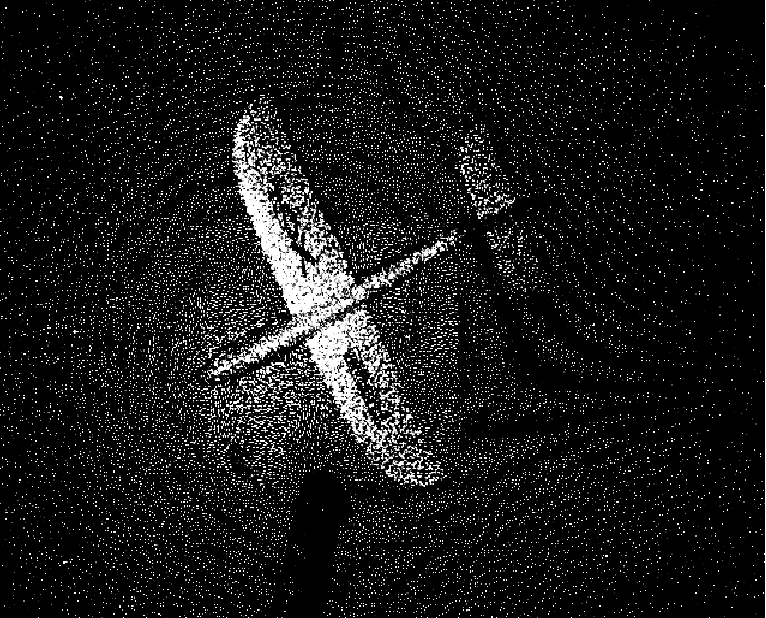
\includegraphics[width=0.45\textwidth]{Bilder/IR_Pattern.png}}\hfill
	\subfigure[Depth data resulting from the IR image]{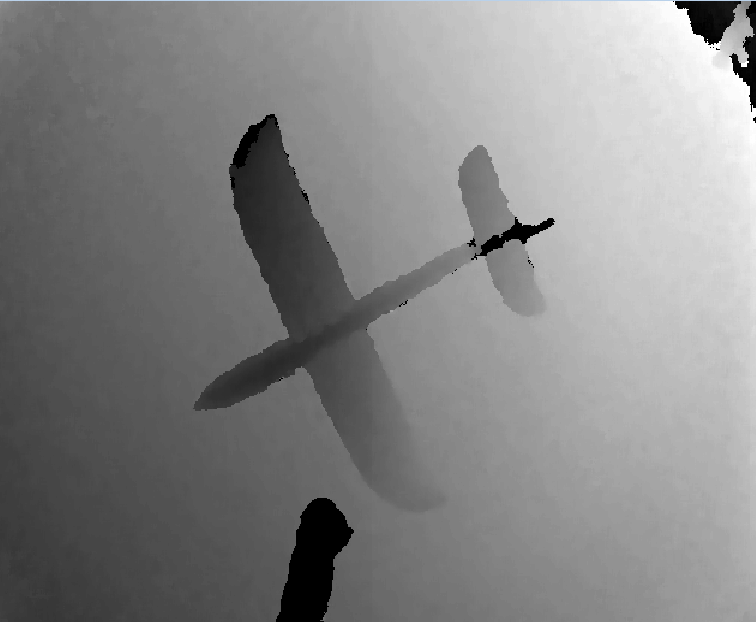
\includegraphics[width=0.45\textwidth]{Bilder/depth_pattern.png}}
	\caption{Kinect 1 structured light}
	\centering
	\label{fig:Kinect1_structured_light}
\end{figure}
\newpage

\subsubsection{Interferometry}
The Doppler effect is the change in frequency that occurs when the observer moves relative to the wave direction. In the interferometry this effect is used to measure the absolute velocity $v$ of an objects relative to stationary coherent light sources with a constant frequency $f_E$. The interference between the reflected and the emitted light results in a new waveform. The interfering light has the new frequency $f_D$ that is proportional to the speed $v$ of the reflecting body. A photo diode measures the sum of the spectral components $f$ and can therefore calculate the frequency shift \cite{CLVpolytec}.

\begin{equation}
f= f_D \pm \frac{1}{\lambda}
\end{equation}

\begin{equation}
f_D=\frac{2\cdot|v|}{\lambda}
\end{equation}
\medskip

Laser Doppler vibrometer is an industrial standard measurement approach that uses a single laser beam to derive the velocity of vibrating point on a surface. Small fluctuations in the wavelength of the laser light would decrease the accuracy. Therefore high stable light sources are necessary. The measurement returns the velocity in a single pixel on one point in space. The absolute distance to the objects can not be derived. The integration of the speed over time results in displacement. Thus, only static scenes can be investigated. For the measurement of complete surfaces, the laser beam is adjusted by a mirror. The displacement of a surface cannot be measured in parallel. Every point is acquired with a time delay. The interferometry also allows to determine depth, directly using a technique called phase-unwrapping.  The earth surface is scanned with this technique, known as terrestrial SAR interferometry. The resolution of such a system is the range of $10^{-9}~mm$ under ideal conditions.

\subsubsection{Time-of-Flight}
The Time-of-Flight (ToF) principle describes a variety of methods that measure the time that a wave or a particle needs to travel an unknown distance. With the constant speed of light $c$ and the measured time of flight $t_{ToF}$, the way that a photon has traveled can be calculated. The established Light Detection and Ranging (LiDAR) 3D scanner uses this technique to measure the distance $d$ to an object with a single laser beam. A laser diode emits a movable beam, which is reflected backwards and measured within a photo diode. The light travels two times the distance $d$ back and forward:

\begin{equation}
d=\frac{c\cdot t_{ToF}}{2} 
\end{equation}
\medskip

The measurement of an absolute distance that can be derived to velocity and acceleration without further information is one advantage of the Time-of-Flight method in comparison to the interferometry. The resulting 3D images is merged together by the sum of pixels that are captured in series over the field of view. The laser beam is readjusted by a movable mirror for every captured pixel. This allows the scan of a complete static scene. Since the image cannot be scanned in parallel but in series, movement between individual measurements results in errors that can be compared to the rolling shutter effects of image sensors. \\ 

New IR global shutter CMOS sensors, in contrast, are able to acquire the total reflecting light in parallel on multiple pixels. Most ToF Cameras use near-infrared ($\approx 850~nm$) LEDs or laser diodes that illuminate the scene. The incident power density falls off with the square of distance according to equation \ref{eq:solid_angles}. The phase shift between the illumination and the reflection is measured and translated into a distance. Every measurement delivers up to three images: The depth, the intensity and in some cases the amplitude of the reflection. Two different method can be found to detect the time between the emitted and the reflected light. The pulsed method uses a single amount of light that is reflected in the room. The emitter illuminates for a brief moment $\Delta t$ and the reflecting light is sampled in parallel in every pixel in two out-of-phase windows over the same $\Delta t$. Both electrical charges $Q_1$ and $Q_2$ are used to compute the distance: 

\begin{equation}
d=\frac{1}{2}\cdot c \cdot \Delta t \cdot \frac{Q_1}{Q_1+Q_2}
\end{equation}
\medskip

The continuous-wave (CW) approach modulates a square or sinus function on the light intensity. Very sensitive single-photon avalanche diodes are able to measure the phase shift $\varphi$ for every pixel with high speed counters. In contrast to the pulsed approach, the waves are measured over multiple periods to derive the phase shift.

\begin{figure} [!h]
	\centering
	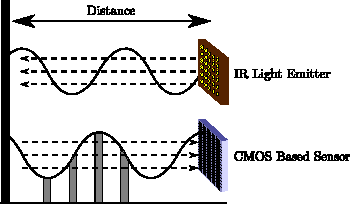
\includegraphics[width=0.5\linewidth]{Bilder/ToF_Principle.pdf}
	\caption{Principle of Continuous-wave Time-of-Flight \cite{foix2011lock}}
	\label{fig:tof_reflection}
\end{figure} 

The time window for the CW measurement is the integration time. It is comparable to the exposure time of an ordinary image sensor. Figure \ref{fig:tof_reflection} illustrates a radiated and reflected square wave IR signal and four phase shifted time windows. $Q_1$ to $Q_4$ represent the amount of charges that are collected in every window. In contrast to the pulsed control, the ambient light can be canceled out by measuring it out of the phase to the IR Signal \cite{litime}.

\begin{figure} [!h]
	\centering
	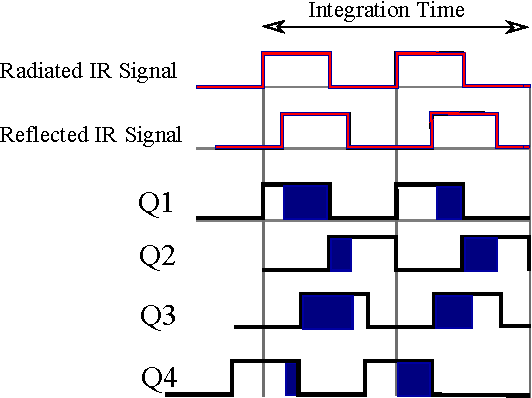
\includegraphics[width=0.5\linewidth]{Bilder/TOF_timing_diagram.pdf}
	\caption{Measuring windows of continuous-wave ToF}
	\label{fig:CW_principle}
\end{figure} 

\begin{equation}
\varphi = \arctan \frac{Q_3 - Q_4}{Q_1 - Q_2}
\end{equation}

\begin{equation}
d=\frac{c}{4\cdot \pi \cdot f}\cdot \varphi
\label{eq:ToF_distance}
\end{equation}
\medskip

The reflected amplitude A and the ambient light offset B are proportional to the depth measurement variance $\sigma^2$:

\begin{equation}
\sigma^2=\frac{c}{4 \cdot \sqrt{2} \cdot \pi \cdot f} \cdot \frac{\sqrt{A+B}}{c_d \cdot A}
\label{eq:variance}
\end{equation}\medskip

Equation \ref{eq:variance} shows that the variance can be reduced with a higher modulation frequency $f_{mod}$ and amplitudes A. The constant $c_d$ is a indicator, how well the ToF sensor separates and collects the photoelectrons. The amplitude can be increased with shorter distances to the scene or with a higher radiant intensity. One disadvantage of the CW measurement is that the phase warps around every $2\pi$. The ambiguity results in multiple possible distances. The intensity of the reflecting light helps to identify the true distance. This limits the range that can be observed. A reduction in the modulation frequency would increase the ambiguity distance but reduce the accuracy at the same time. With the maximum phase shift angle $\varphi = 2\cdot\pi$ and equation \ref{eq:ToF_distance}, the ambiguity distance can be calculated by the following equation:\\

\begin{equation}
d_{amb}=\frac{c}{2\cdot f_{mod}}
\end{equation}
\medskip

Ambient light in the same IR spectral region disturbs and results in noise. A monochromatic filter in front of the lens can reduce the incident light to the wavelength of the emitting diodes. Unfortunately, the sunlight emits in a broad bandwidth that cannot be filtered out completely.\\

 In comparison to the other range imaging techniques, ToF has the advantage of a small size, no moving parts, a high range and a very fast scanning speed. The only disadvantage is the low depth accuracy of $1~mm$. New senor developments could increase the resolution significantly down to $0.3~mm$ \cite{thierryoggietof}.

\subsection{Time-of-Flight Imaging Errors} \label{chap:range_errors}
Depth measurement with ToF cameras faces the appearance of both, systematic and non-systematic errors. Generally, systematic errors can be reduced by a calibration \cite{foix2011lock}. This section gives a rough overview of different errors sources and their reasons. 

\subsubsection{Systematic Errors}
\textbf{Range Distortion}\\
The IR light can not be generated in an ideal sinusodial or square waveform, as a consequence range distortion appears. Usually, the error plotted against the distance follows a sinusoidal shape that can be compensated by a calibration. \\

\textbf{Integration-Time-Related Error}\\
Scientific ToF cameras allow to adjust the integration time for the depth measurement. For the same scene, different values cause changes in the results. The precision versus different depths depends on the integration time.\\

\textbf{Build in Pixel-Related Errors}\\
Inaccuracies in the production of the image sensor causes error in the depth measurement. The diodes or capacitors differ in the responsibility and latency-related offset error. This type of errors are related to the position of the pixel on the sensor array. A Fixed Pattern Noise (FPN) table can be created to obtain the computed depth with a reference distance.\\

\textbf{Amplitude-Related Errors}\\
Depth accuracy is highly related to the amount of incident light. High reflected amplitudes result in a high accuracy. Low amplitudes appear more often at the border of the image as the emitted light power is lower. When the object is too close to the camera or the integration time has been chosen to high, saturation appears and the depth measurement will be invalid.\\

\textbf{Temperature-Related Errors}\\
Depth values suffer from the operation temperature of the sensor. After the activation of the camera it is heating up, until it reaches a stable temperature. In this phase, the depth error changes versus time. The camera should be turned on several minutes with activated illumination before the usage to achieve an precise measurement.

\subsubsection{Non-systematic Errors}

\textbf{Low Illuminated Regions}\\
Scenes that are not illuminated uniformly will suffer from regions with low illumination. This causes a high amount of noise and a reduction in the signal-to-noise ratio. The amplitude image can be used to filter out these kinds of pixels.\\

\textbf{Multiple Light Reflection Error}\\
The interference of different light reflection in a single pixel occurs depending on the shape of the scene. Surface edges and concavity reflect the wave in multiple ways. The light travels in successive paths before it reaches the sensor. Therefore, a depth measurement is corrupted. Flying pixels on sharp edges are one artifact that is observed in all ToF 3D scans. Light from the background interferes with the reflection on the edge in the foreground. This result is a noisy pixel that seams to jump in space and cannot be allocated to a connected surface.\\

\textbf{Light Scattering}\\
Reflections with high amplitudes from nearby objects can cause light scattering between the image sensor and its lens. This influences the measurement of other nearby pixels and results in noise. New sensor material with low reflectivity could make scattering negligible in the future.\\

\textbf{Motion Blur}\\
As with traditional cameras, the capture of dynamic scenes results in motion blur, depending on the integration time and the speed of the observed object. The error can be classified in two different types of artifacts: Lateral and axial blur.\\

\textbf{Flying Pixels}\\
False distance information can also occur due to the pixels relative large solid angle. Different distances inside a solid angle lead to superimposed reflected light reducing its amplitude and introducing a false phase shift. These pixels are commonly known as flying pixels, because they lie in-between the fore-and background. 


\newpage
\subsection{Acquisition of Digital Dynamic Data}

The discretization of an analog signal, like from a pixel, is done in the analog to digital converter (ADC). The signal value will be divided into single samples depending on the bit depth $n_{Bits}$ as shown in figure \ref{fig:nyquistthereom} with 3 Bits $\equiv 2^3$ steps. The sampling is controlled by a digital signal with the frequency $f_{sampling}$ that determines the conversion from the analog to the digital value. The Nyquist-Shannon theorem in equation \ref{eq:Nyquist-Shannon Theorem} proves, that the minimal possible sampling frequency $f_{sampling}$ must be double the maximum frequencies $f_{max}$ of the signal to preserve the spectrum. For the estimation of amplitude and slop a factor of two is not enough. A variety of samples per period is required, depending on the shape of the signal, to ensure a sample as near as possible to the peak of the deflection. High resolutions and sampling frequency mean less quantization errors. Therefore, differences between the digital and analog signal gets smaller. The averaging of multiple samples is a common way, used to reduce the noise and the data stream of the acquisition.

\begin{equation}
f_{sampling}\geq f_{nyquist} = f_{max} \cdot 2 
\label{eq:Nyquist-Shannon Theorem} 
\end{equation}

\begin{figure}[!h]
	\centering
	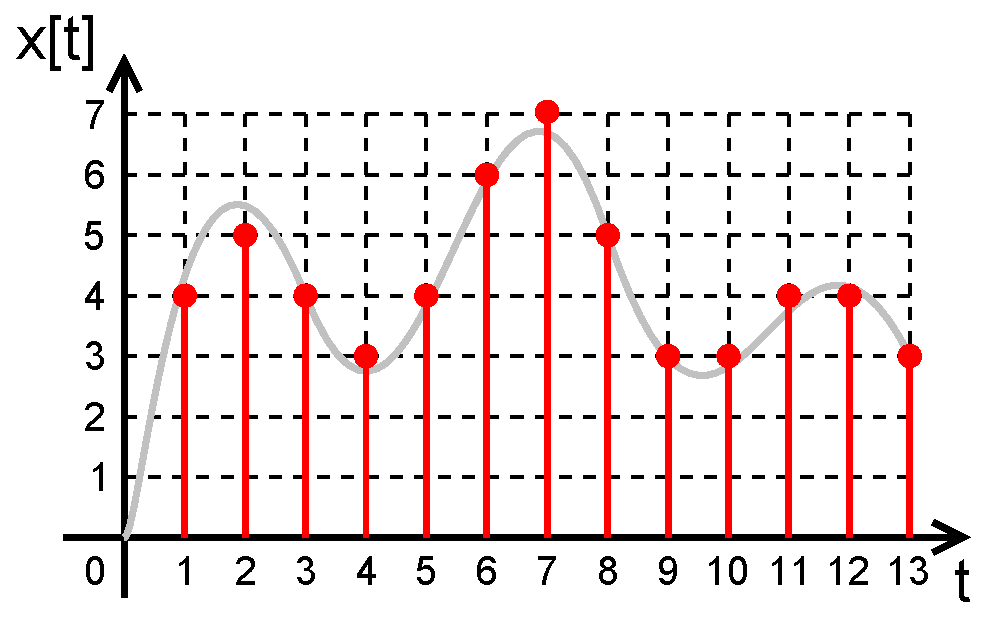
\includegraphics[width=0.4\textwidth]{Bilder/discret.pdf}
	\caption{Illustration of the analog to digital conversion \tiny wdwd wikipedia.org}
	\label{fig:nyquistthereom}
\end{figure}

Higher frequencies above $f_{max}$, resulting from noise or other sources, still have an undesirable impact on lower spectral components. These effects are called aliasing artifacts and lead to artificial frequency components. A low-pass filter applied on the analog signal with a cutoff frequency $f_{max}$ can reduce this phenomenon. Higher frequencies than $f_{max} = f_{sampling}~/~2$ will not arrive at the ADC input.\\

An aperture error results from the fact that the sample is obtained as a time average within a sampling region and not at an instant moment. The effects are corresponding to the motion blur of image sensors. Oversampling is the process of sampling with frequencies much higher than $f_{nyquist}$, leading to an improved resolution and less quantization noise. For an accurate measurement of the amplitude, a minimum sampling frequency of $f_{sampling} = f_{nyquist}\cdot 5$ is used in practice, to reduce influences like aperture errors or aliasing. The factor between the $f_{nyquist}$ and $f_{sampling}$ dimension is called Oversampling Factor N. The data stream of a ADC converter can be calculated by the sampling frequency $f_{sampling}$ and the digital resolution $n_{Bits}$ by the following equation:

\begin{equation}
\dot n = n_{Bits}\cdot f_{sampling} ~ [\frac{bit}{s}]
\label{eq:datastream} 
\end{equation}
 
\subsection{Evaluation of Dynamic Data}

\subsubsection{Time Domain}
The analysis of mathematical function with respect to time is called time domain. The time is represented in form of real numbers, for the case of continuous time or in discrete number resulting in a discrete time. An oscilloscope is a common tool for the investigation of real-world signals in the time domain. The graph describes how a value changes with time, whereas a frequency-domain graph describes how much of the signal amplitude lies within a given frequency band versus a range of frequencies. Certain terms are used for the description of the time domain. Figure \ref{fig:sinus} shows different properties of a sinus oscillation.  

\begin{figure}[!h]
	\centering
	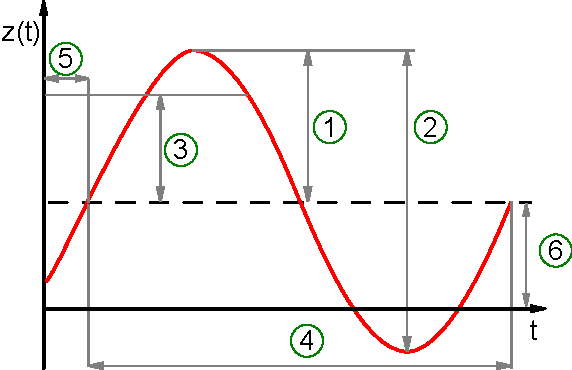
\includegraphics[width=0.4\textwidth]{Bilder/Sine_oscillation.pdf}
	\caption{Properties of sinus oscillation \tiny Saure wikipedia.org}
	\label{fig:sinus}
\end{figure}

\begin{enumerate}
\setlength\itemsep{0.001em} 
\item Peak amplitude $A_{p}$ - Maximum absolute value from zero to highest values
\item Peak-to-peak amplitude $A_{pp}=A_{p}\cdot 2$ - Change between highest value and lowest amplitude value
\item Root mean square amplitude $A_{rms}=A_{p}/\sqrt{2}$ - The square root of the mean versus time of the square in the vertical distance of the graph
\item Wave Periode $T=\frac{1}{f_{p}}=\frac{2*\pi}{\omega}$ - Time difference between one periodic oscillation
\item Phase Shift $\varphi$ - Time difference between the $t=0$ and the zero crossing of the oscillation or another reference time
\item Offset $Z_{DC} $ - Constant displacement from the origin to the equilibrium
\end{enumerate}	
	
An undamped sinus oscillation can be described in two mathematical forms: One is the common analytic sinus form as a function of time $t$. The value $Z_{DC}$ is a static offset in the coordinate system that superimposes the dynamic by a constant static value. In this case, the oscillation is not around the point of origin but around the equilibrium.

\begin{equation}
z(t)=A_{p}\cdot \sin(~2\cdot\pi \cdot f \cdot t + \varphi~) +Z_{DC}
\end{equation}  

The oscillation can also be represented with the help of the Euler equations and imaginary numbers. The imaginary part has no physical meaning, but it simplifies the processing of a dynamic function.
\begin{equation}
\bar{z}(t)=A\cdot e^{j(\omega\cdot t +\varphi)} + Z_{DC}
\end{equation}

The energy keeps constant at a free undamped sinus oscillation:

\begin{equation} \label{eq:Energy_oscillation}
E=\frac{1}{2}~m\omega^2 A^2
\end{equation}



\subsubsection{Frequency Domain} \label{chap:frequency_domain}
Every steady periodic function can be transformed into a sum of sinus oscillations, by a so called Fourier transformation. This allows the investigation and the comparison of dynamic signals. To do so, the data is transformed from the time domain $z(t)$ into the frequency domain $|Y(f)|$. The signals can now be investigated without a common time base. The frequency domain is represented by a spectrum that shows the individual amplitudes components versus the corresponding frequencies. This can be especially useful in the analysis of vibrations of structures. Undesired eigenmotions can be compared and analyzed. In figure \ref{fig:FFT_principle}, the waveform of equation \ref{eq:noise_fft} is illustrated, which is superimposed by some random noise.

\begin{equation} \label{eq:noise_fft}
z(t)= 0.7\cdot sin(2\cdot \pi\cdot 50~Hz \cdot t) + 1.4\cdot sin(2\cdot\pi\cdot 120~Hz \cdot t) + y_{noise}
\end{equation}

The two sinus wave forms and the noise are difficult to separate in the time domain. In the frequency domain, in contrast, noise and the original function can be distinguished. The two peaks indicate that the original function consists of two sinus functions with 50 Hz and 120 Hz. The noise floor lies underneath with multiple random peaks in the whole spectrum. The amplitudes from the original signal converge with the peaks in the frequency domain over a longer timespan and a higher $f_{sampling}$. More detailed information on this example can be found in the official Matlab documentation of the fft() function \cite{Matlab_FFT}.

\begin{figure}[!h]
	\subfigure[Time Domain]{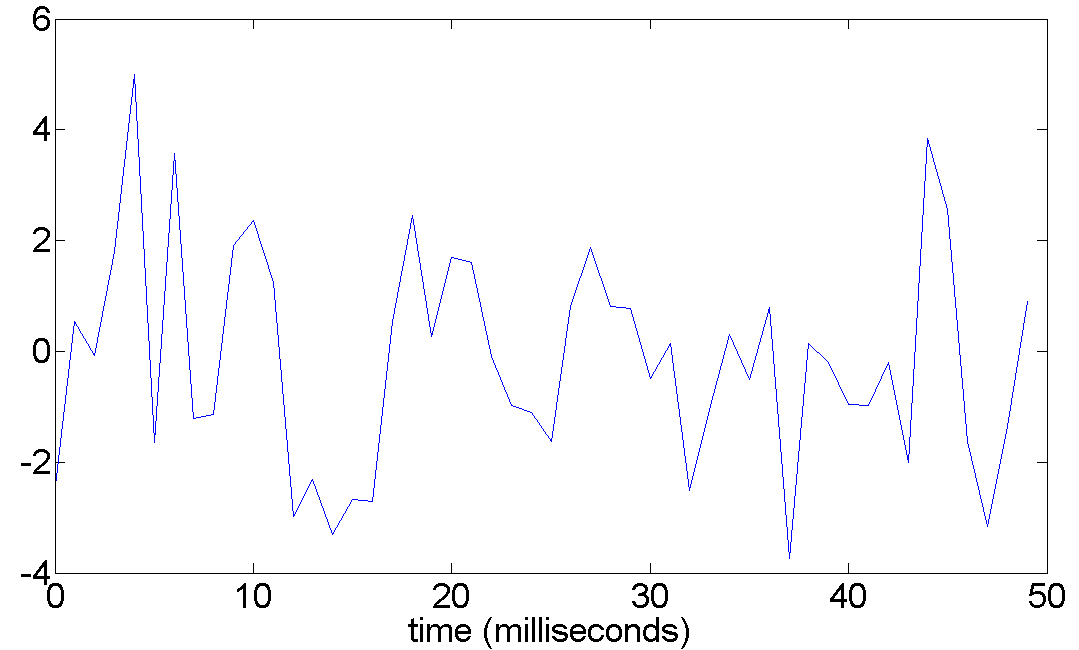
\includegraphics[width=0.5\textwidth]{Bilder/FFT_example_timedomain.png}}\hfill
	\subfigure[Frequency Domain]{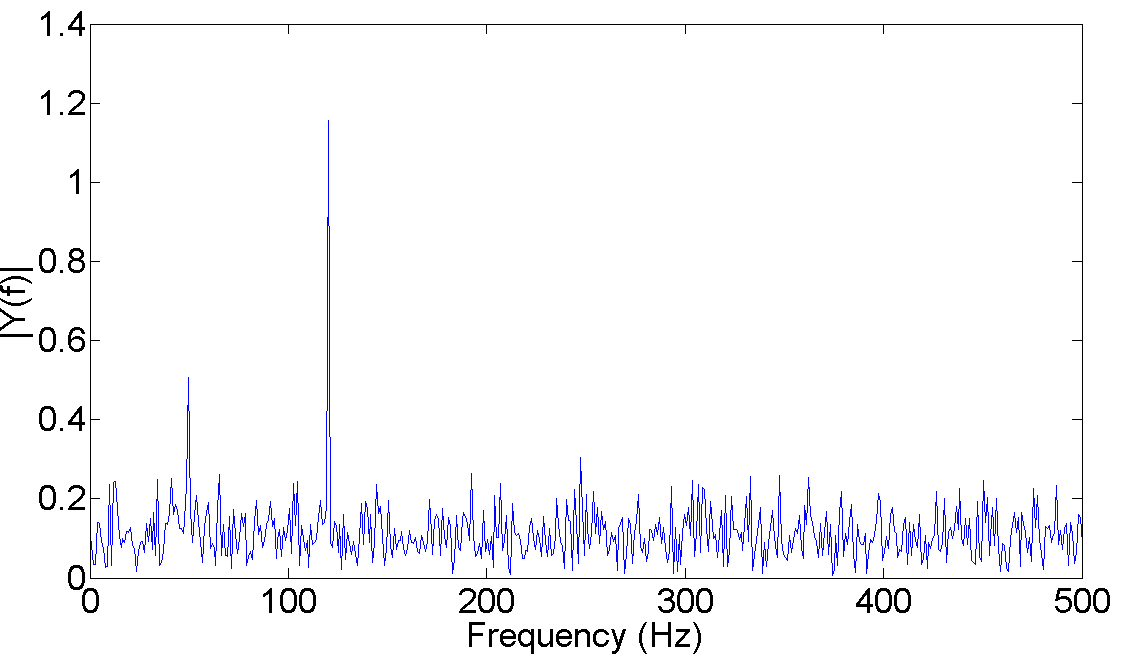
\includegraphics[width=0.52\textwidth]{Bilder/FFT_example_freqdomain.png}}
	\caption{Fast Fourier Transformation in Matlab}
	\centering
	\label{fig:FFT_principle} 
\end{figure}

The Fast Fourier transform (FFT) is a widely used algorithm to convert a digital signal from one domain into another. The input data must be in a discrete digital form with $2^n$ samples. In this way, the processing power is much lower compared to the original Discrete Fourier Transform (DFT). The signal is transformed into its complex components. The real parts of the frequencies represents half of the sinus function amplitude. $f_{sampling}$ of the computed signal must be known to calculate the right frequencies out of the raw data. The following code is take from the fft() example and plots the frequency domain out of the raw data array y with the number of elements L:

\begin{lstlisting} 
NFFT = 2^nextpow2(L); % Next power of 2 from length of y
Y = fft(y,NFFT)/L;
f = Fs/2*linspace(0,1,NFFT/2+1);
plot(f,2*abs(Y(1:NFFT/2+1)))
\end{lstlisting} 

NFFT contains the number of samples that are processed. Y is half of the amplitudes while f provides the corresponding frequency array that goes from zero to $f_{nyquist}$. These data are plotted against each other. The single-sides amplitude is two times the real part of the complex representation of the amplitude components from Y.\\
 
The original digital signal can be reproduced from the frequency domain into the time domain without any loss through the inverse fast Fourier transform. This is useful for the filtering of data. Undesired frequency components can be identified and removed from the data.
When the FFT of a non-periodic signal is computed, the resulting spectrum suffers from leakage. This can occur when only parts of a period are measured at the start or the end of the acquisition. The variance of the spectrum increases. Different FFT windows are used to reduce the influence of signal at the beginning and ending, like the hammington window \cite{proakis2001digital}. When measuring a self-windowing signal, like an impulse, a shock response, a sine burst or a noise burst a window should not be used. Such signals are used in modal analysis. Applying a window function would just deteriorate the signal-to-noise ratio.\\

The Short-time Fourier Transform (STFT) is used to determine the sinusoidal frequency and phase content of local sections of a signal as it changes versus time. Therefore variation versus time can be analyzed better than with the FFT of the complete signal. The Matlab function spectrogram() delivers a way to create a STFT out of a signal. The trend of amplitude and frequency is plotted versus time in intervals that are represented by NFFT as a number of samples for a separated Fourier Transform. The overlapping factor describes the range between two windows that is analyzed by both. The following source code represents an example for the creation of a spectrogram in Matlab:

\begin{lstlisting} 
 Fs = 30; %Samplingrate
 amp=2;%peak-Wert
 zeitmax=5;
 zeit=linspace(0,zeitmax,zeitmax*Fs);
 daten=amp*sin(2*pi*zeit*frequenz)
 nfft = 32;%Blockgroesse 2er-Potenz
 window = hanning(nfft);
 % z.B. 80 fuer 80% overlap
 Prozent_overlap = 5;
 overlap = round(nfft/100)*Prozent_overlap;
 [B,F,T] = spectrogram(daten,window,overlap,nfft,Fs)
 figure
 imagesc(T,F,abs(B));
 colormap(jet);
 colorbar
 axis xy
 ylim([0 30])
\end{lstlisting} 
 

\newpage

%	Hauptteil
\section{Time-of-Flight Market Research}

Since the semiconductors technology became fast enough for the development of ToF cameras in the year 2000, multiple companies developed image sensors for civil applications. The following section shall give an overview of the ToF cameras that are currently on the market or will soon be released. Detailed specifications like resolution, size, accuracy, hardware/software trigger and integration times can be found in the official associated datasheets. In the following table specifications of sample image sensors and complete camera systems from the industrial and consumer market are gathered:
\begin{center} 
	\begin{tabular}{| l | l | l | l | l | l | l |}
		\hline
		 & Pixel Array & Speed [fps] & FOV [$^\circ$] & Range [m] & Size [mm]  \\ \hline
		 Mesa SR4000 & 176x144 & 30 & $69x55$ & $8$ & $65x65x76$  \\ \hline
		 pmdtec CamBoardpico & 160x120 & 45 & $82x66$ & $1$ & $89x17x6$ \\ \hline		 
		 Fotonic E70 16W & 160x120 & 52 & $70x53$ & $30$ & $80x80x86$  \\ \hline
		 Argos 3D - P100 & 160x120 & 160 & $90x90$ & $3$ & $27x75x57$  \\ \hline
		 odos real.iZ-1K & 1280x1024 & 100  & not fixed & $10$ & $182x80x92$ \\ \hline
		 Basler ToF-6c & 640x480 & 30 & $48x38$ & $5$ & - \\ \hline
		 Microsoft Kinect 2 & 512x424 & 30 & $70x60$ & $8$ & $249x66x67$ \\ \hline
		 Polytec epc660 Sensor & 320x240  & 264 & - & $240$ & - \\
		 \hline	
	\end{tabular} \captionof{table}{Time-of-Flight camera systems}	
\end{center}
 The Argos 3D - P100 camera offers a high frame rate of 160 fps at a low depth resolution and number of pixels. It also has a hardware trigger which makes it useful for synchronization with other devices. Multiple sensors can be synchronized phase shifted to each other. The interaction of the IR light between different sensors is therefore prevented. The Real.iZ-1K brings the highest fps with the largest number of pixels. In contrast to the other system the pulsed wave ToF approach is used. Additional illuminators can be added to the camera to increase the accuracy at high distances. The standard C mount allows the exchange of the lens. Therefore, the field of view can be adjusted. The high flexibility of this system requires a calibration before it can be used. The output data must be preprocessed by a calibration matrix to obtain depth data. A trigger input allows the synchronization with other systems. The Fotonic E70 shows good motion blur characteristics and is the only sensor based on CCD technology. It is designed for rough environments and shows good outdoor characteristics. The company pmdtec offers ToF cameras, such as the highly compact Camboard Pico and the Camboard Nano, where the lenses and illuminators are fixed. Since there is no hardware trigger, a synchronization frame by frame is not possible. Mesa SR4000 is one of the pioneer in ToF technology. Lots of scientific work has been published based on this system. Basler is a new player is this sector, offering the first prototype with a high number of pixels at 30 fps and an external trigger. The Development of image senors with $1280x1024$ is already announced. Microsoft brings ToF with the Kinect 2 into the consumer market. Compared to the other industrial system, the price is very low with $200~\$$ for a complete development kit. Nevertheless the resolution, range and accuracy can still keep up. A higher frame rate and range has been implied \cite{payne20147} \cite{sell2014xbox}. A disadvantage is the absence of raw data access and low level configurations. Polytec makes a huge advantage with the image sensor epc660. 264 fps at 320x240 pixels should allow the investigation of fast dynamic scenes. A region of interest enables 4000 fps at 160x30 pixels and therefore various applications in the investigation of fast unsteady deformations. Currently there is no operational camera on the market with this sensor. Overall, the ToF market is rapidly growing. The cancelling of ambient light will allow outdoor applications soon, since companies like pmdtec are interested in outdoor application in the automotive industry. The increase in range, frame rate, depth resolution and number of pixels over the last few years enables many of industrial, civil and scientific applications. 

 \begin{figure}[!h]
 	\centering
 	\fbox{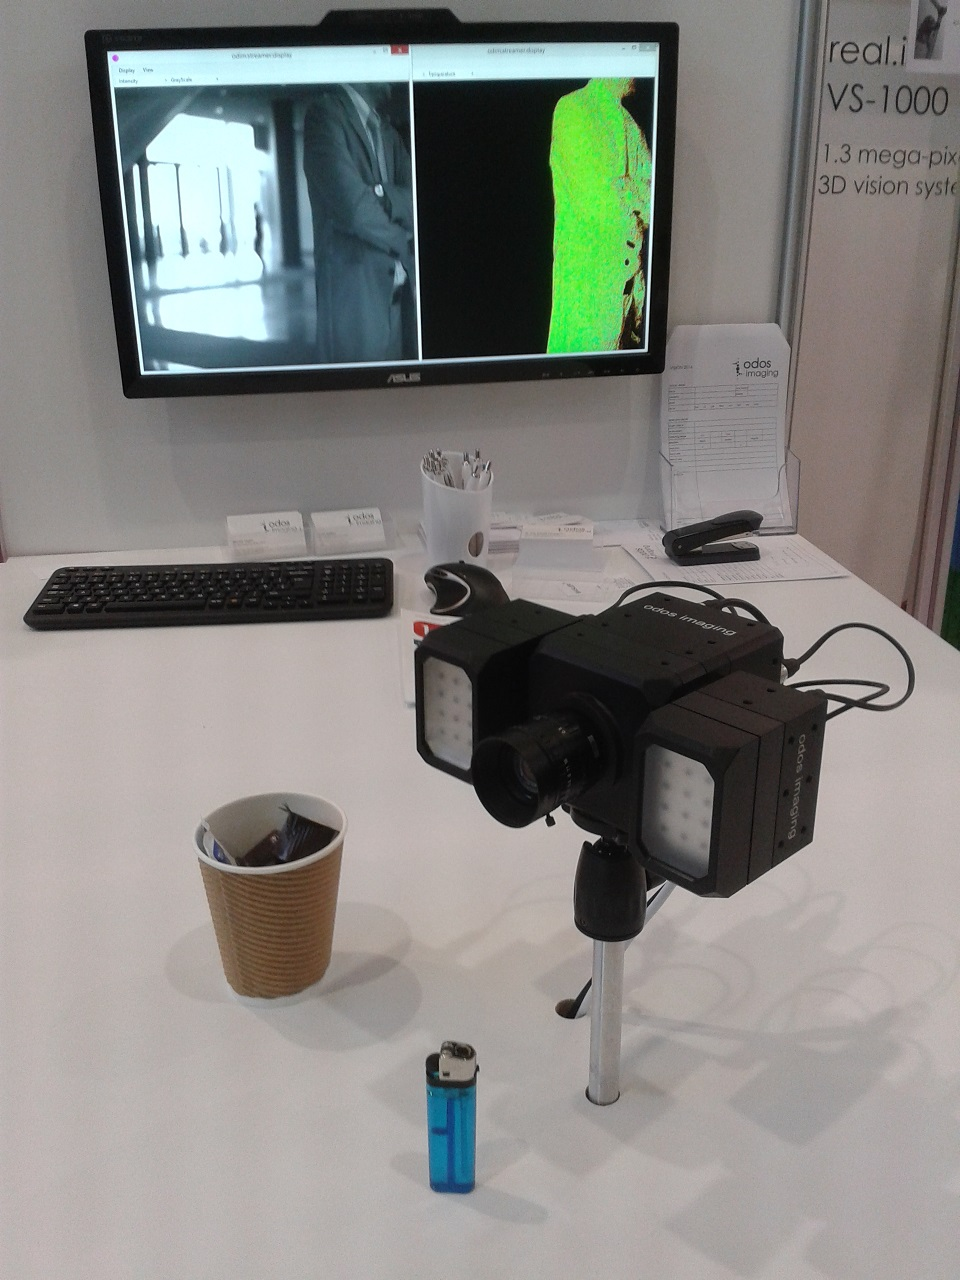
\includegraphics[width=0.37\linewidth]{Bilder/odos.jpg}}
 	\caption{odos real.iZ-1K 1280x1024 with changeable lens and illuminator}
 	\label{fig:odos_real_iK_1K}
 \end{figure} 


\subsection{Kinect 2 System Overview}
The Kinect 2 is the first Time-of-Flight consumer camera and brings the highest total amount of pixels compared to other ToF devices at the time of the release. It is originally designed for gesture recognition and enables the control of games and other applications by hand or body movements. This thesis concentrates on the ToF camera even if other sensors are included, like a microphone array and a HD CMOS rolling shutter camera for visible light. In contrast to the Kinect 1, the developer decided to change the technique of the range imaging from a structured light sensor to Time-of-Flight. This increases the accuracy, field of view, resolution, number of pixels and the maximum distance. Thus movements of multiple persons can now be captured in parallel and applications can be controlled by the users even by figure gestures. No official technical specifications of the sensor have been released yet. In Payne's publication, an image sensor is presented that probably is the one, which is integrated in the camera \cite{payne20147}. The following table represents the basic specifications from the publication:
\medskip

	\begin{center}
    \begin{tabular}{| l | l |}
    	\hline
    	Pixel Pitch & $10~u*10~u$  \\ \hline
    	Chip Size & $8.2~mm*14.2~mm$  \\ \hline
    	Pixel Array & $512 x 424$  \\ \hline
    	Dynamic Range & $>2500=68~db$  \\ \hline
    	Modulation Frequency & $10-130~MHz $ \\ \hline
    	Average Modulation Frequency & $80~MHz$ \\ \hline
    	Field of View &  70 (H) x 60 (V) degrees  \\ \hline
    	Depth Uncertainty & <0.5 $\%$ of range \\ \hline
    	Operating Wavelength & $860~nm$ \\ \hline
    	Frame Rate &  max. $60~fps$ (typical $30~fps$) \\ \hline
    	ADC Data Stream & $2~GS/s$ \\ \hline
    	Effective Fill Factor & $60\%$ \\ \hline
    	Reflectivity &	$15\%-95\%$ \\ \hline
    	Responsivity @ $860~nm$ & 0.144 A/W  \\ \hline 
    	Readout Noise	& $320~uV$ differential \\ \hline 
    	ADC Resolution & $10~Bits$ \\ 
    	\hline 
    \end{tabular} \captionof{table}{Kinect 2 system specifications}	
\end{center}
\newpage

The illumination is based on three $860~nm$ IR laser diodes. A rough measurement of the emitted light with a single IR photo diode and an oscilloscope showed that the diodes flash with a rate of $30~Hz$. The frame rate of the depth video stream also corresponds to $30~fps$, visible in figure \ref{fig:Kinect2_photodiode} and \ref{fig:Photodiode_measurement_kinect_3frequencies}. Every IR flash period comes with a burst of three different intensities and frequencies of $120~MHz$, $80~MHz$ and $16~MHz$ for a time of approximately $5.4~ms$ resulting in one depth frame \cite{sell2014xbox}. After about $16~ms$ of IR light, the diodes are turned off for $16~ms$ and a new image is created. The captures are taken in rapid temporal succession to avoid motion blur. Every image results out of three different modulation frequencies to achieve the high dynamic range over large distance from $0.5~m$ to $8~m$. Microsoft does not allow low level hardware access yet to change the modulation frequency or integration time.
The sensor diodes feature a responsivity of $0.14~ A/W$ at the laser wavelength. To increase the fill-factor to $60\%$, micro lenses are integrated into every pixel for a larger detecting area. With the given lens speed of 1.07, the focal length is approximately $80~mm$ with a aperture measured by hand of about $70~mm$. Figure \ref{fig:Kinect2_optic} shows a Kinect 2 disassembled. The three laser diodes are heavily shielded. The beam is scattered and filtered by the optic in front of the diodes. The IR camera lens and the case are equipped with monochromatic filters. Disturbing IR light sources such as the sun are reduced in this way.\\ 
 
 \begin{figure}[!h]
 	\centering
 		\fbox{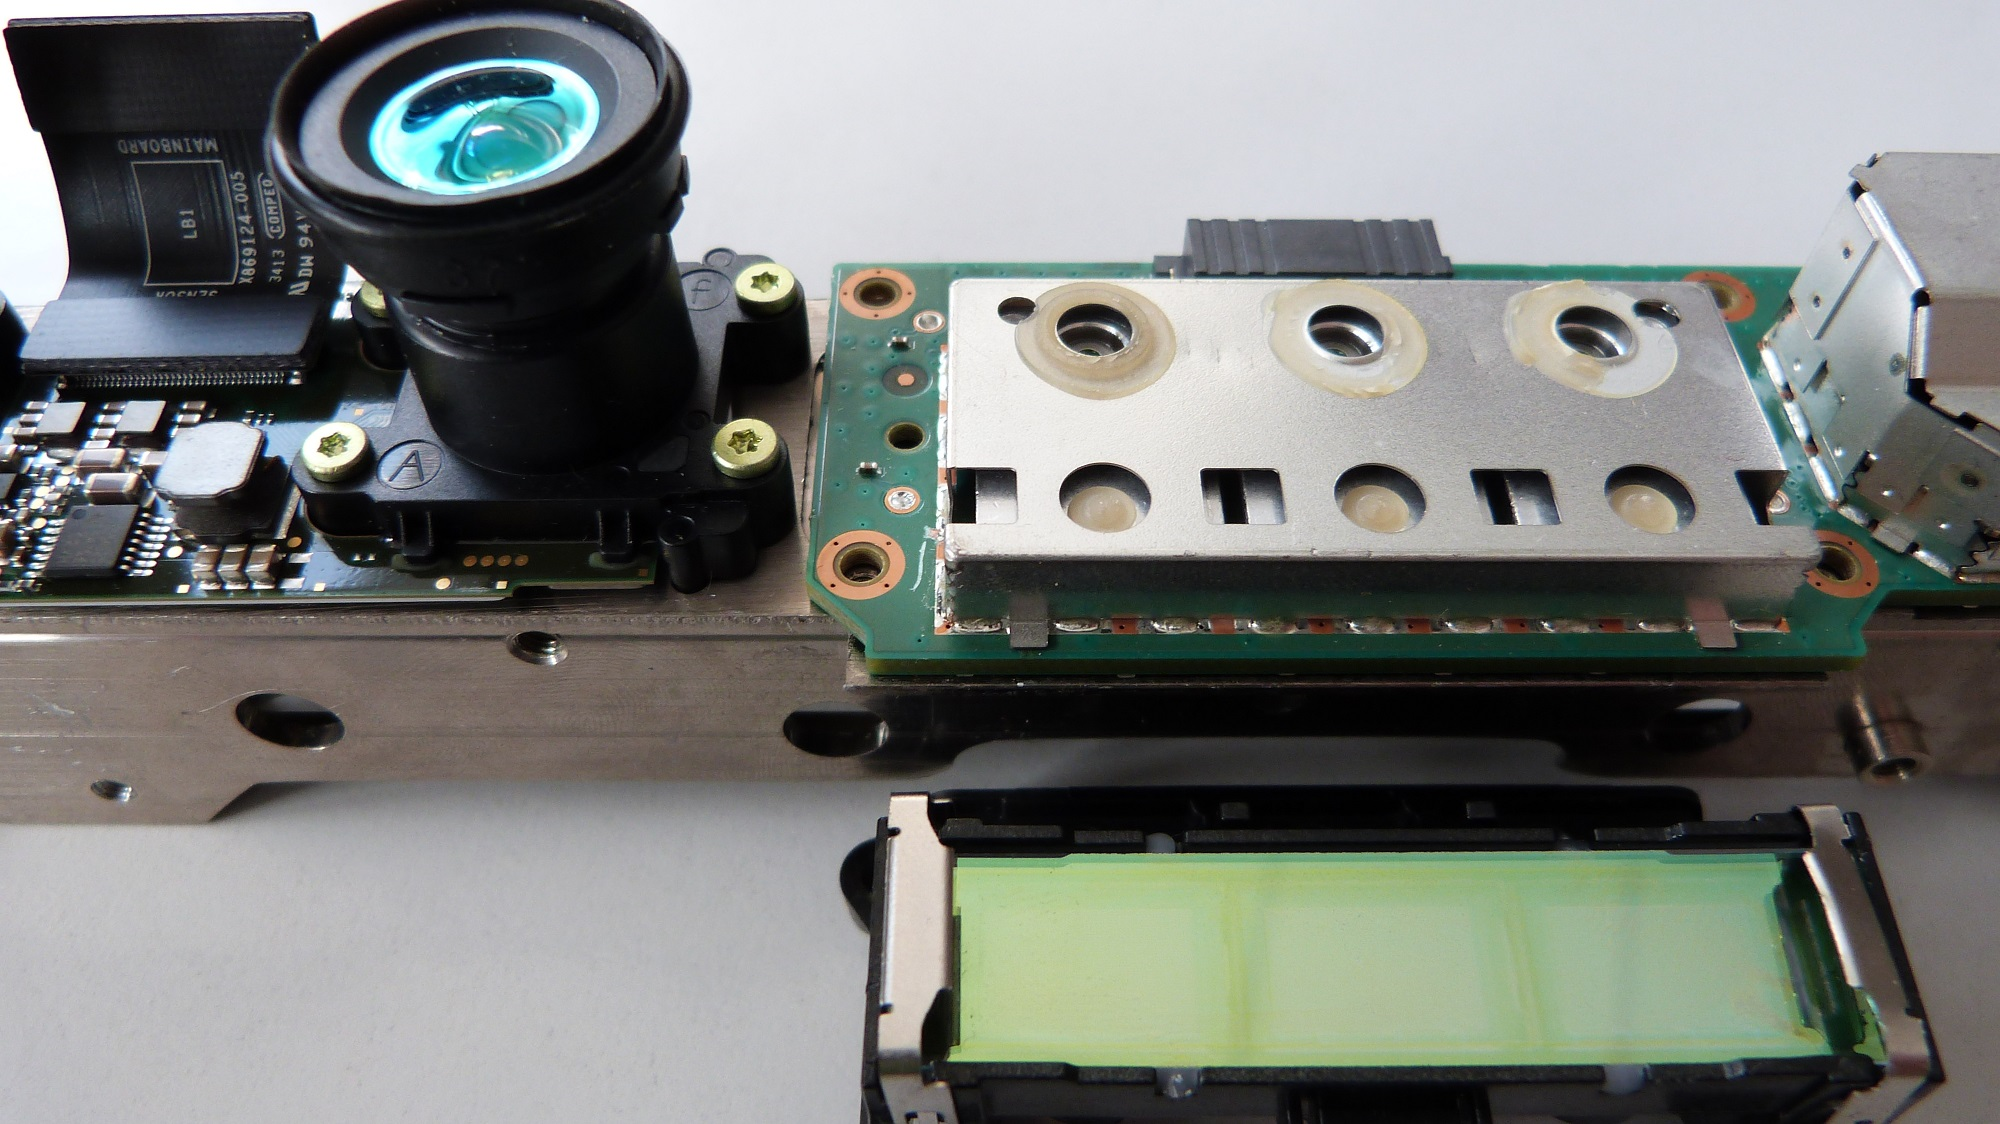
\includegraphics[width=0.8\linewidth]{Bilder/IR_camera.jpg}}
 	\caption{Kinect 2 IR camera and IR illumination with scattering optic }
 	\label{fig:Kinect2_optic}
 \end{figure} 
 

A high dynamic range is necessary to simultaneously render high-reflectivity objects near the camera and low-reflectivity objects far from the camera to provide the depth resolution for all pixels. Every pixel selects the best shutter time and amplifier (AMPs) gain for the ADCs by itself. The digitized output from the ADCs is combined in the shutter engine. The MIPI interface provides the communication to other embedded systems. Figure \ref{fig:Kinect2_ImageSensor} shows a microscope image of the Kinect 2 Image Sensor. The electronic for the processing of the data is located on the sides to avoid interferences with the image sensor, common on modern CMOS sensors.\\

\begin{figure}[!h]
	\centering
	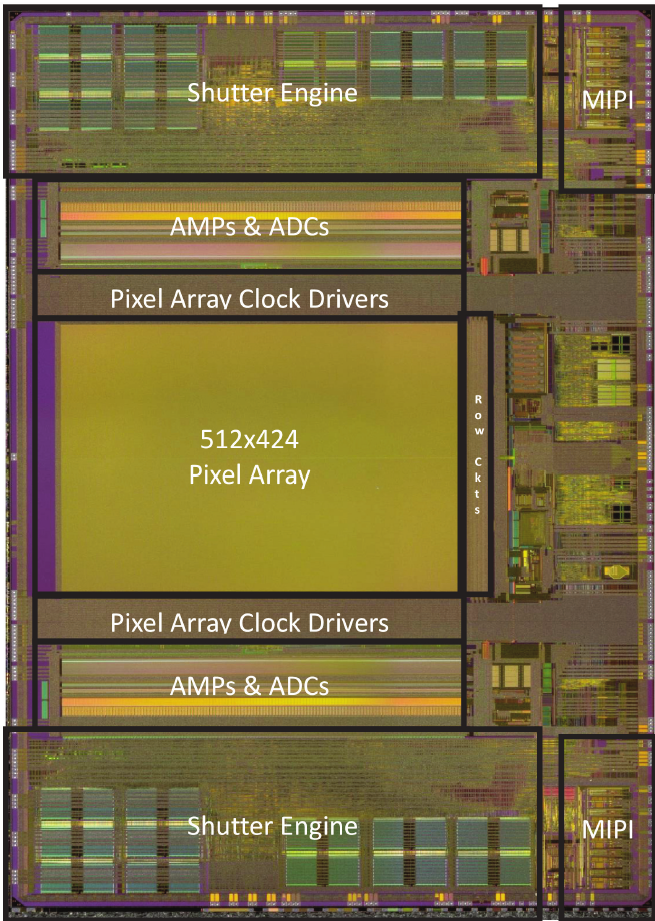
\includegraphics[width=0.5\textwidth]{Bilder/Kinect2Sensor.png}
	\caption{Kinect 2 image sensor \cite{payne20147}}
	\label{fig:Kinect2_ImageSensor}
\end{figure} 


A USB 3.0 connection allows the readout of the images with a latency less than $20~ms$. A $12~V$ power supply delivers additional power to the camera when it is plugged to a computer. The data and the power supply are combined in a proprietary cable. Thus, the Kinect Hub is required to use a standard USB 3.0 plug for the PC connection. With the Microsoft Software Kinect 2 Studio, the data steam can be observed in a 3D point cloud but direct access to raw data is not possible in this application. Microsoft offers the Kinect for Windows Development Kit 2.0 to create customized programs for the processing of the Kinect 2 data stream. Several demonstration programs with source code in $C++$ and $C\#$ are included but raw data acquisition of a complete video stream is not provided yet. Wai Ho Li offers the first open source tool dumpK4W that saves the "raw" data from the video stream to a mass storage \cite{dumpk4W}. These images are given in an integer resolution in millimeters and therefore the data stream must already be processed by the camera itself. Wai Ho Li uses the OpenCV library for real-time computer vision to save every picture from the data stream. The images cannot be processed in real-time for further investigations. A driver for the Matlab environment would be useful for a real-time processing.\\

The field of view of the IR camera is fixed to one lens position. Adjustment of the focal length is not possible. The advantage for the user is, that the system can be calibrated before it is shipped to the customer. A calibration before the operation of the camera is therefore not necessary. The range images are converted into millimeters inside the camera before they are transfered via USB. The area $A$ that is observed by the sensor in a certain plain results out of the distance and the angle of view $\theta$ in the horizontal and vertical direction: 

\begin{equation}\label{eq:lfov}
l_{h,v} = \tan{\frac{\theta_{h,v}}{2}}\cdot d \cdot 2~[m]
\end{equation}

\begin{equation}\label{eq:area}
A = l_v\cdot l_h = \tan{\frac{70^\circ}{2}}\cdot \tan{\frac{60^\circ}{2}} \cdot d^2 \cdot 4~[m]
\end{equation}
\medskip
The area projected on a single quadratic pixel $A_i$ is the fraction of one pixel to the complete area $A$. Figure \ref{fig:FOV} illustrates the field of view, the distance to the observed scene d, the coordinate system of the observed plane (index p) and the camera (index c).

\begin{equation}
A_i = \frac{A}{512\cdot 424}~[m^2]
\label{eq:pixel_area}
\end{equation}

\begin{figure}[!h]
	\centering
	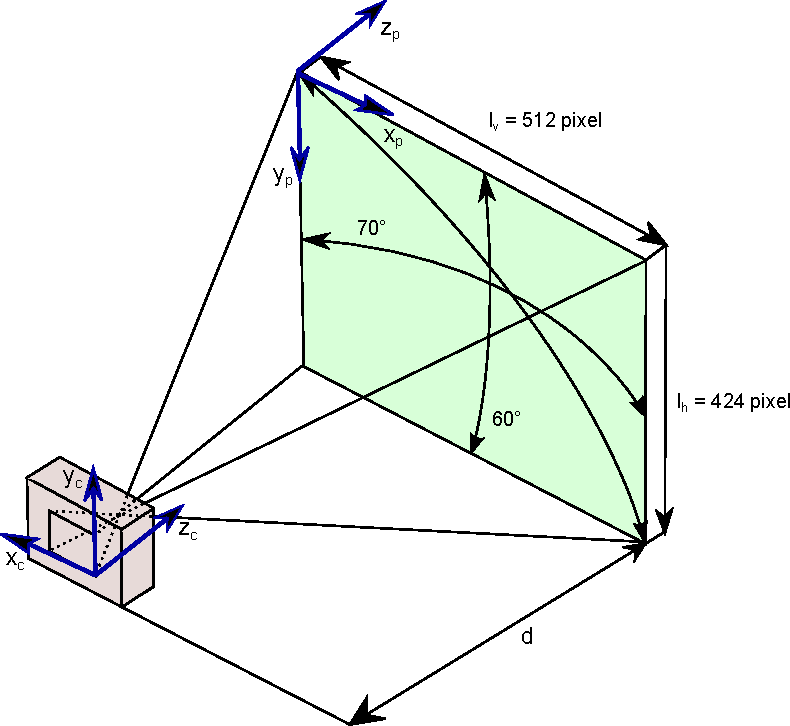
\includegraphics[width=0.53\textwidth]{Bilder/425px-Angle_of_view.pdf}
	\caption{Kinect 2 field of view}
	\label{fig:FOV}
\end{figure} 


\section{Data Processing of Range Images}
The video stream, saved with dumpK4W, consists of a bunch of individual pictures. A frame rate of $30~fps$ every second of acquisition will result in 60 images from the IR camera. One capture is represented in a depth and intensity image. The data is given in the Tagged Image File Format (TIFF) in 512x424 pixel with a non-standard aspect radio. TIFF is a common format for the lossless storage of image data. The pixels consist of a $16~Bit$ integer number that represents the distance in millimeters to the image plane. About 13 bits are used corresponding to the $8000~mm$ of maximum distance. Values under $500~{mm}$ and beyond $8000~{mm}$ are set to zero. 
 When opened in a standard image viewer, the files seem to be only black. The brightness and the contrast must be changed to foreground the shades of grey to distinguish different pixels. Matlab provides a set of tools for the processing of the raw data. The Matlab Image Processing Toolbox delivers a variety of ways for the processing of images and video streams. It is widely used in scientific environment and features offline and live processing of image data. Figure \ref{fig:imagesc} represents a raw image that is plotted with the imagesc() function in Matlab.  

\begin{figure}[!h] 
	\centering
	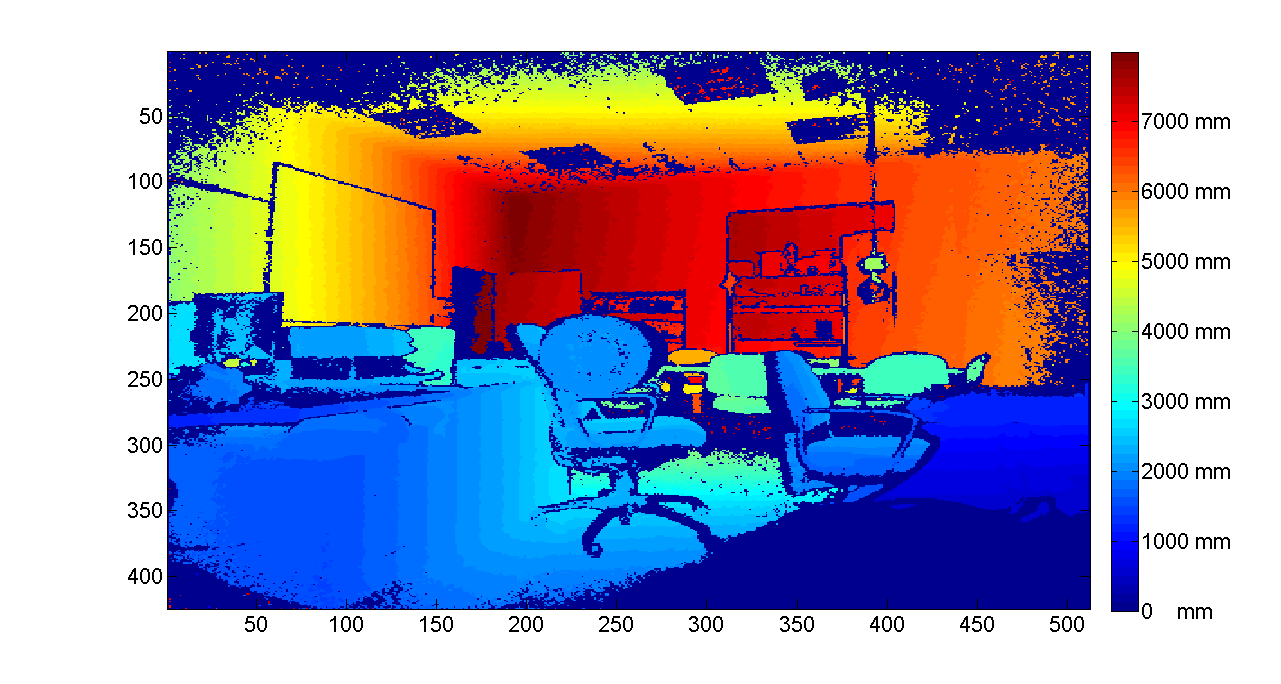
\includegraphics[width=1.0\textwidth]{Bilder/2m_bass_office.png}
	\caption{Raw image plotted with imagesc() function}
	\label{fig:imagesc}
\end{figure}   

The distance is represented in a red, green and blue colorspace that is fitted to the depth resolution. Red indicates far distances and blue the near fields. Isolines in the color space show equal regions of distance. Figure \ref{fig:imagesc} shows, that the depth values are given perpendicular to the image plane. The isolines run parallel to the image plane, possible due to the fixed calibrated focal length and simplifies the processing of the data considerably.
Noise is one of the major challenges in the interpretation of ToF Data. It can be considered as an unwanted fluctuation of the range measurement error. The noise increases at the corners of the FOV. This is caused by the optic of the camera and the light cone of the illumination. The lens reduces the light intensity at the outer boarders of the image. The threshold in this area can barely be archived and therefore the Signal-to-Noise ratio is reduced. The live display of the point cloud in Kinect Studio can be used for a rough estimation of the noise. The pixels seem to jump when observed live on a static surface. A detailed analysis of the noise characteristics can be found in section \ref{sec:static_evaluation}. The orientation of the raw data is flipped in the vertical axis, since it is given in the camera coordinate system. The Matlab command fliplr() transforms the image into the observed plane coordinate system.

\subsection{Transformation into Point Cloud Data}
The data must be transformed into a so called point cloud to gain 3D information out of the 2D data. The images are already given in a calibrated form happens inside the camera. Other camera devices with adjustable FOV, low level configuration and flexible illumination need a calibration of the raw images into the corresponding distance. Systematic errors are reduced in this way \cite{lindner2010time} \cite{lefloch2013technical}. Every pixel in the $512x424$ array corresponds to a single point in 3D space, depending on the field of view and distance. Kinect Studio enables to rotating of live point cloud data. The regions which are not reached by the IR light, are highlighted in the form of shadows. Figure \ref{fig:pointcloud} shows one frame of the video stream that is shifted to the perspective of the camera. The person in the foreground shows an ideal diffuse reflection of the IR light and therefore a high signal-to-noise ratio. The transformation into a point cloud from raw data is also possible with the open source program MATLAB to Point Cloud Library (PCL) created by Peter Corke. It delivers a bundle of tools for visualization, surface reconstruction, filtering and segmentation. It is a standard environment for 3D image processing, that is developed by companies from different industries.

\begin{figure}[!h]
	\centering
	\fbox{\includegraphics[width=0.9\textwidth]{Bilder/pointcloud.png}}
	\caption{Point cloud in kinect studio}
	\label{fig:pointcloud}
\end{figure}  


\newpage
\subsection{Meshing of Point Cloud Data}
For the reconstitution of a scanned object, 3D points are not enough. The point cloud needs to be meshed. The vertices in the form of points represent knots for this connection. The lines in between are called edges. A face is a set of edges that can be combined into a closed surface. Figure \ref{fig:Mesh_overview} shows the transformation of a cube from vertices to triangle faces. 

\begin{figure}[!h]
	\centering
	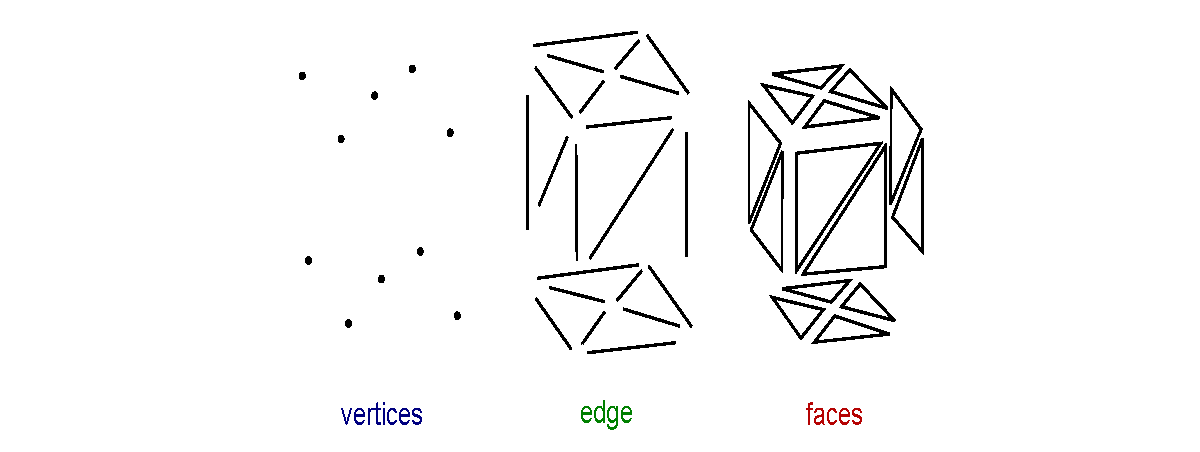
\includegraphics[width=0.8\textwidth]{Bilder/Mesh_overview.pdf}
	\caption{Transformation from vertices into faces \tiny Rchoetzlein wikipedia.org \ccbysa}
	\label{fig:Mesh_overview}
\end{figure}

Kinect Fusion is a Simultaneous Localization and Mapping (SLAM) algorithm which is capable to mesh the ToF video stream in real time. It is designed for accurate real-time mapping of complex and arbitrary indoor scenes. The algorithm is capable to recalculate the camera's orientation and position when it is moved. In the Kinect Fusion Explorer Demo, Microsoft allows the export of this data into a mesh format like the Surface Tesselation Language (STL). It is a standard interface that is supported by most 3D programs for further processing. 
Stlwite is another tool for Matlab to create STL files from the raw depth data. Figure \ref{fig:AC_meshing_Meshlab} shows a single frame of an aircraft model that is taken with the Kinect 2 camera, transformed into STL with Matlab and imported into the Open Source program Meshlab. Data from the far background and foreground was removed from the point cloud in Meshlab. The flying pixels at the edges lead to "flying surfaces" after the meshing of the raw image. 

\begin{figure}[!h]
	\subfigure[Meshlab]{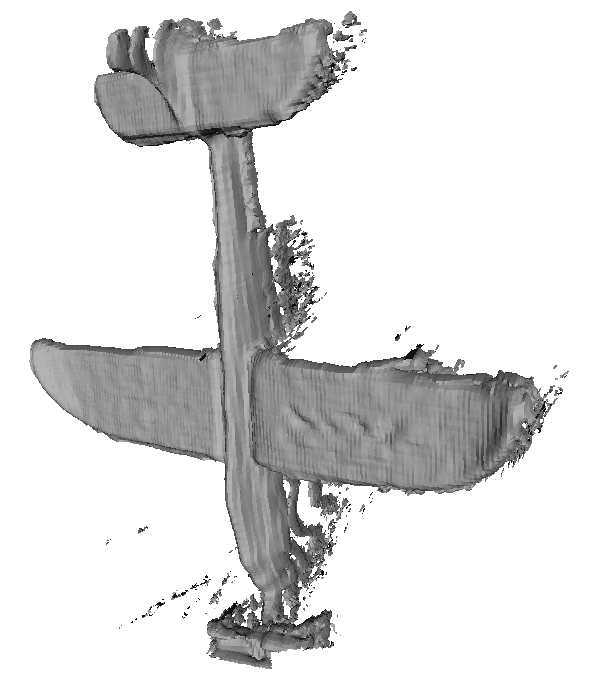
\includegraphics[width=0.4\textwidth]{Bilder/meshedaircraft.png}\label{fig:AC_meshing_Meshlab}}\hfill
	\subfigure[Matlab]{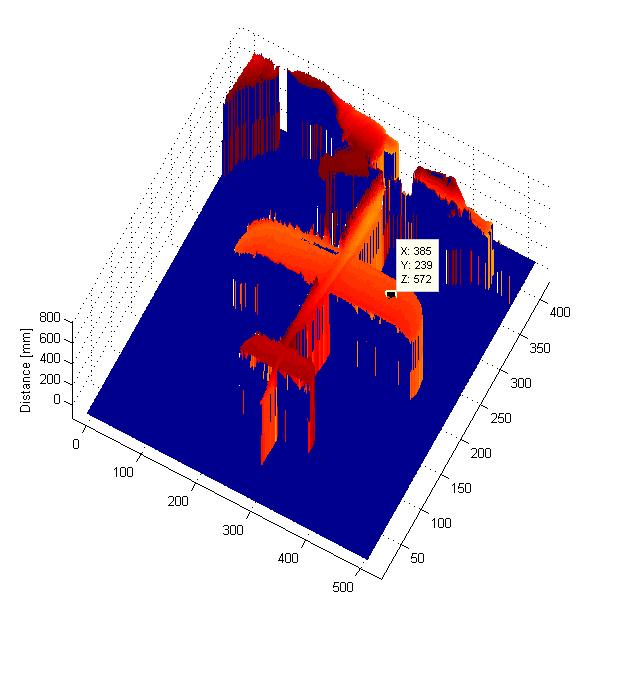
\includegraphics[width=0.6\textwidth]{Bilder/ACMesh.png}\label{fig:AC_meshing_Matlab}}
	\caption{Meshing of point cloud data}
\end{figure}

The camera must be moved to provide a complete 3D scan of an object from all sides. To fuse multiple images into a single 3D space, the orientation of the object to the camera must be know. Reconstruct Me and other software toolkits offer the scan of a room or objects from different points of view. The position of the moving camera is calculated out of the video stream. By merging the range data from all sides, the 3D scape is reconstructed. 

A simple construction of mesh data from range images can also be done in Matlab. The function mesh(Z) draws a wireframe with a surface color corresponding to the Z axis. It is a simple and fast way to determine the quality of the raw data. Before the meshing of the image, it needs to be transformed in double values by the function double(). For a reduction in processing time, the data can be reduced to the distance of the investigated object. Measurements in other regions are cut out. The data cursor in an already plotted mesh helps to identify this value by the user. Figure \ref{fig:AC_meshing_Matlab} shows the resulting plot and the cursor to identify the region of interests with a cut off distance of 800 mm.
\medskip
\begin{lstlisting}
Imagedouble = double(ImageInteger)
Imagedouble(Imagedouble > CutoffDistance) = 0
mesh(Imagedouble)
\end{lstlisting}

\
\subsection{Analysis and Filter Methodes} 
 Multiple filtering approaches are made, to improve the quality of the image data. They all have in common that they aim to remove the measurement noise which results from different types of error specified in section \ref{chap:range_errors}. Fluctuations between multiple depth images are useful to separate noise from the so called ground truth image. 

\subsubsection{Creation of Frame Arrays} \label{chap:Framearray}
For the processing of a video stream the single pictures have to be aligned into a single matrix that consists out of the rows times columns times number of images L. 90 frames for example recorded in $3~s$ create an 512x428x90 3D matrix called Framearray. The data is gathered from a folder that contains all depth images. For keeping them in the right order, they have to be numbered consecutively in the file name. The time delta between two frames correspond to $T_{sampling} =\frac{1}{fps}$. The following code shows how to create an array of frames in Matlab out of an image folder. The images are transfered into double data type from unsigned integer.
\medskip
\begin{lstlisting} 
ImageFolder=uigetdir('C:\ImageFolder','Folder RAW Data Images');
L=length(dir(strcat(ImageFolder,'\*.tiff')));
for g = 1:L
	Frame=double(imread(strcat(ImageFolder,'\',tiffFilesS(g).name)));;
	Framearray(:,:,g) = Frame;
end
\end{lstlisting} 

\subsubsection{Mean and Variance}
The ground truth image is simply the mean of all data from the stream. Noise in the depth information is canceled out by multiple measurements. This is a standard way to remove non-systematic noise for a higher precision. The additional parameter in the function declares the dimension over which the matrix is averaged. The number of images determines the quality of the result. In some publications up to 500 images are used. Movements in the recording time corrupt the resulting image.
\medskip
\begin{lstlisting}
GroundTruthImage = mean(Framearray,3) 
\end{lstlisting} 
\medskip
The variance of a single pixel depth measurement versus time determines how much the value fluctuates around the mean value. With the ground truth image as the expected value $\mu$ the variance \ref{eq:var} of a single pixel can be derived with the Var() function:
\medskip
\begin{lstlisting}
PixelVariance = var(Framearray(Colume,Row,:));
\end{lstlisting}

\begin{equation}\label{eq:var}
\sigma^2(X)=Var(X)=\sum_{n=1}^N (x_i -\mu)
\end{equation}

The variance for an complete depth image plotted into a new image provides a simple way to estimate noise characteristics of different material. Figure \ref{fig:variance_raw} represents the variance of a scan on wooden plane area in a distance of about $700~mm$. Values with a higher variance than 7 mm are set to zero. The reason for that is the high amount of noise in the corners of the image. The variance reaches values up to $470~mm$, corresponding to the low radiant flux and darkening of the lens in the corners. The distribution is separated in elliptic uniform regions. The middle of the field of view shows the lowest variance. The variance increases in the image's corner direction. Apart from the corners, the variance alternates between 2 mm to 0.8 mm. In a box between 100 to 450 pixel horizontal and 50 to 350 pixel vertical the mean variance is 1.205 mm. Source code \ref{list:FFT} demonstrates the principle how the variance image can be created. The mean variance in a pixel area delivers a single value that is better comparable.

\begin{figure}[!h]
	\centering
	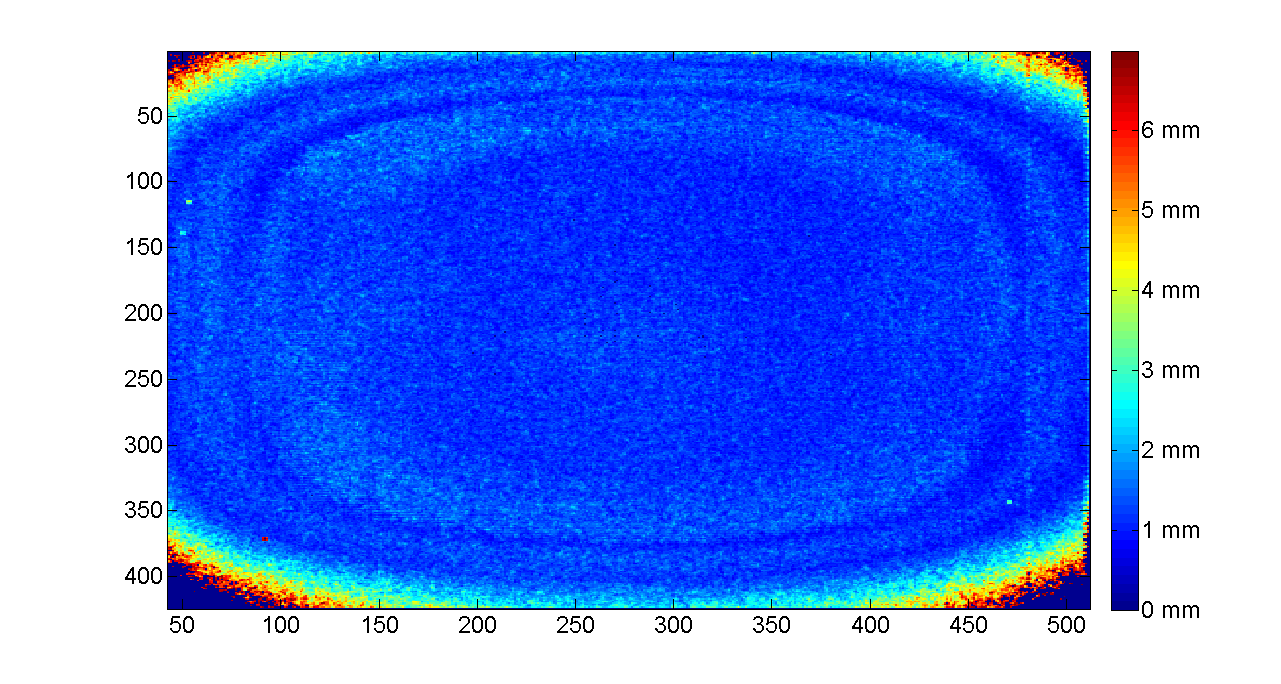
\includegraphics[width=0.85\textwidth]{Bilder/variance_platte_07m.png}
	\caption{Raw variance of an wooden plate in $700~mm$ distance}
	\label{fig:variance_raw}
\end{figure}

\newpage

\subsubsection{Gradient}
The gradient of an image specifies the alteration in the 2D data space. Mathematically the gradient of a two-variable function at each image pixel is a 2D vector with the components given by the derivatives in the horizontal and vertical direction. At each image point the gradient vector points in the direction of the largest possible intensity increase. The length of the vector is a measure for the rate of change. The gradient of an image is given by the formula with x pointing in the horizontal and y in the vertical direction:

\begin{equation}\label{eq:grad}
\nabla f = \frac{\delta f}{\delta x} \hat{x} + \frac{\delta f}{\delta y} \hat{y}
\end{equation}
\medskip
\begin{lstlisting}
[Gmag,Gdir] = imgradient (Frame)
\end{lstlisting}
\medskip

The corresponding Matlab function imgradient() contains the magnitude of the vector Gmag and  the direction Gdir in degree to the vertical axis. The following Figure \ref{fig:gradient_magnitude} shows the image gradient of the office room. Values above $200~mm$ have been cut off to fit the colorspace and to highlight small differences.

\begin{figure}[!h]
	\centering
	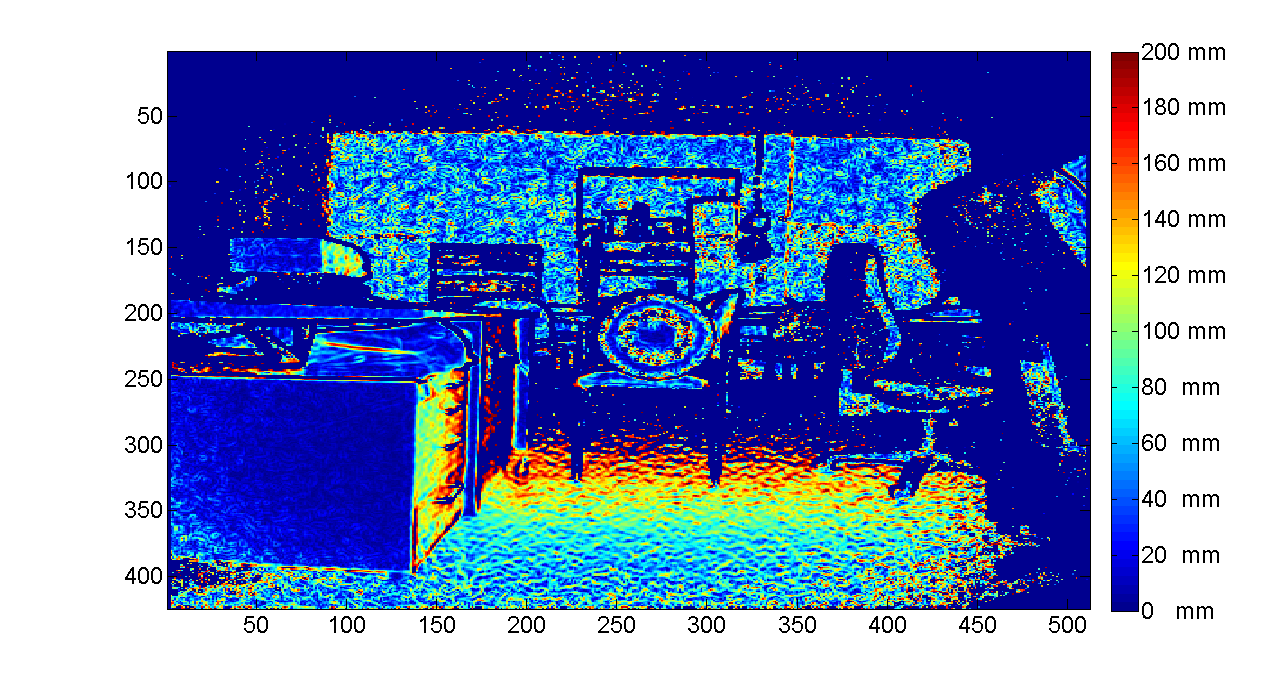
\includegraphics[width=1\textwidth]{Bilder/OfficeGradientMag.png}
	\caption{Gradient magnitude of the office room}
	\label{fig:gradient_magnitude}
\end{figure}

The cupboard in front of the image stands parallel to the image plane. That is why the gradient is small. The floor features small changes in the foreground and with higher distance the magnitude increases. At the end of the room with a distance of $6812~mm$ the noise increases the gradient. Ideally, the flat wall should show only one constant value like the cupboard in the foreground. In general, high angles to the image plane will result in high gradients and low angles in small ones. This can be useful in different subjects. Edges around surfaces and planes are recognized. Flying pixels can be removed from the image, since they feature a high gradient to nearby pixels. Plane regions with various gradients conclude to areas with low reflectance or saturation of the image. The flat area in the middle shows a very low gradient and is therefore perpendicular to the sensor plane. 

\subsubsection{Denosing with Mean or Median of a Pixel Area}
One basic approach to reduce the noise in the depth data is the mean or median between nearby pixels. The depth is smeared to a single value. Such kind of filtering benefits from the Kinect's high number of pixels. The median sorts every element by its value and takes the middle element. Therefore, the impact of outlier can be reduced. The mean sums up every value and divides it by the number of elements. The following source code shows the calculation of a median and a mean value from a pixel area:

\begin{lstlisting} 
for g = 1:NumberOfPictures
    k=0;
    for a=1:v_windowlength 
   		for b=1:h_windowlength
   		k=k+1;
   		Pixelsector(k) = FramearrayDyn_Raw(v_edge+a,h_edge+b,g);                
    		end
    end
    DynPixelMean(g) = mean(Pixelarea); 
    DynPixelMedian(g) = median(Pixelarea);
 end
\end{lstlisting}

A pixel area with the vertical dimension v$\_$windowlength and horizontal dimension h$\_$windowlength is collected in the array Pixelsector. The postion is determined by v$\_$edge and h$\_$edge. DynPixelMedian collects the median value of this area for every pixel.
   
\subsubsection{Total Variation Denoising}

Rudin et al. pioneered the Total Variation Denosing (TVD) filter method that suppress noise profiles like Gaussian noise. In contrast to other approaches, like linear smoothing or median filtering, TVD simultaneously preserves edges whilst smoothing away noise in flat regions, even at low signal-to-noise ratios. It is based on the principle that signals with excessive and possibly disturbing details have high absolute gradients \cite{rudin1992nonlinear}. With a given signal, the absolute gradient can be calculated by the following formula:

\begin{equation}
V(X)=\sum_{n} |(x_{i+1} - y_n)|
\end{equation}

One measure of closeness is the sum of square errors:

\begin{equation}
E(x,y)=\frac{1}{2}\sum_{n} (x_n - y_n)^2
\end{equation}

The aim of TVD is to minimize the following discrete functional versus the function $y_n$:
\begin{equation}
E(x,y_n)  + \lambda V(y_n)
\end{equation}

The regularization parameter $\lambda_r$ controls the impact of the total variation on the smoothing. A high value will minimize the total variation while small values will preserve the original signal. Figure \ref{fig:TVD_1D} plots a noisy signal and the filtered curve after TVD.

\begin{figure}[!h]
	\centering
	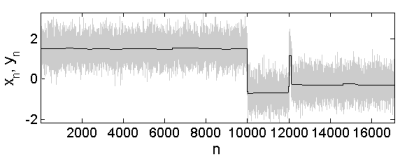
\includegraphics[width=0.5\textwidth]{Bilder/TVD_1D_Example.png}
	\caption{Total Variation Denoising of a 1D signal \tiny MAL 2010 wikipedia.org \ccbysa}
	\label{fig:TVD_1D}
\end{figure}

Noise from 2D data like range images helps significantly in the reduction of different noise qualities. An adaptive TVD approch is proposed based on an extended structure tensor using the amplitude and phase of the ToF signal as reference \cite{lenzen2011denoising}. In contrast to other filter methods, depth noise is removed from the 3D shape, while edges are still preserved. This algorithm has been implemented by Guy Gilboa into Matlab \cite{TVD_Matlab_code}. $\lambda$ is set to one by default. The number of iterations is adjustable. Even if we cannot access the phase and amplitude of ToF data, the filter can still be used on the raw images with fixed parameters. Figure \ref{fig:variance_TVD} illustrates the variance of the same data which figure \ref{fig:variance_raw} is based on. The TVD filter significantly reduced the mean variance of the complete plate from $1.205~mm$ to $0.1540~mm$ based on 20 iterations and $\lambda_r =1$. The circular isolines of variance are highly reduced. Except for the corners, the variance could be reduced.

\begin{figure}[!h]
	\centering
	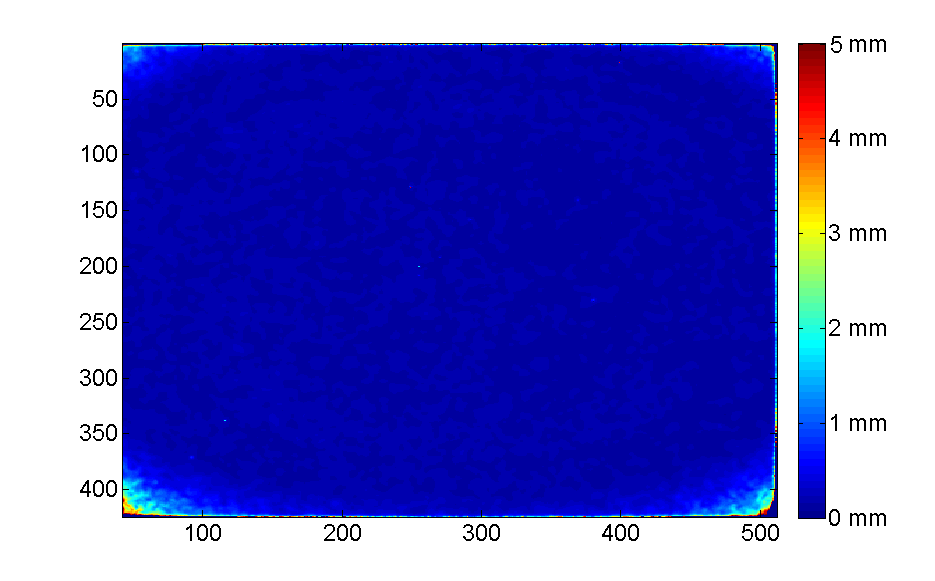
\includegraphics[width=0.9\textwidth]{Bilder/variance_platte_07mTVD.png}
	\caption{TVD filtered variance of an wooden plate in $700~mm$ distance}
	\label{fig:variance_TVD}
\end{figure}

\newpage
\subsubsection{Processing of Dynamic Depth Data} \label{sec:Dynamic_pixel}
The range information that is represented in the whole picture allows an dynamic investigation on every region of the field of view. For this purpose, the amplitudes of the noise must be smaller than the dynamic that is investigated. The number of images should correspond to $2^n$ for the FFT algorithm. If this is not the case, the remaining data is set to zero, fitting to $2^n$ samples. A new 2D array with the depth of every frame is created to investigate a single pixel over the complete video stream. Afterwards, the static offset of the data to the image sensor plane is removed. Every value of the array is reduced by the mean of the whole data set. Following this, the dynamic is investigated without the static offset to the surface. This process can be done for every pixel in the field of view. It remains a video stream, which contains just the dynamic. Out of this, new images are generated that represent the amplitude or frequency of the maximum peak in the spectrum. Source code \ref{list:FFT} shows how to create frequency and amplitude images out of the FFT. The variable $f_{p}$ represents the frequencies between zero and the maximum possible value of $15~Hz$. AmpsDyn contains the amplitudes $A_{p}$ divided by four and is given in the same dimension as the frequency array. The abs() function removes the complex values which result from the FFT and only the real part remains. The max() function returns the maximum values from the spectrum that we need to create the images for the $f_{p}$ frequency and $A_{p}$ amplitude distribution. Figure \ref{fig:Leinwand_FFT} illustrates the maximum amplitudes of a canvas in a frame that is excited with about $5~Hz$ by a student over 8 seconds. Higher values than $40~mm$ have been cut out to distinguish small changes in the color space.

\begin{figure}[!h]
	\centering
	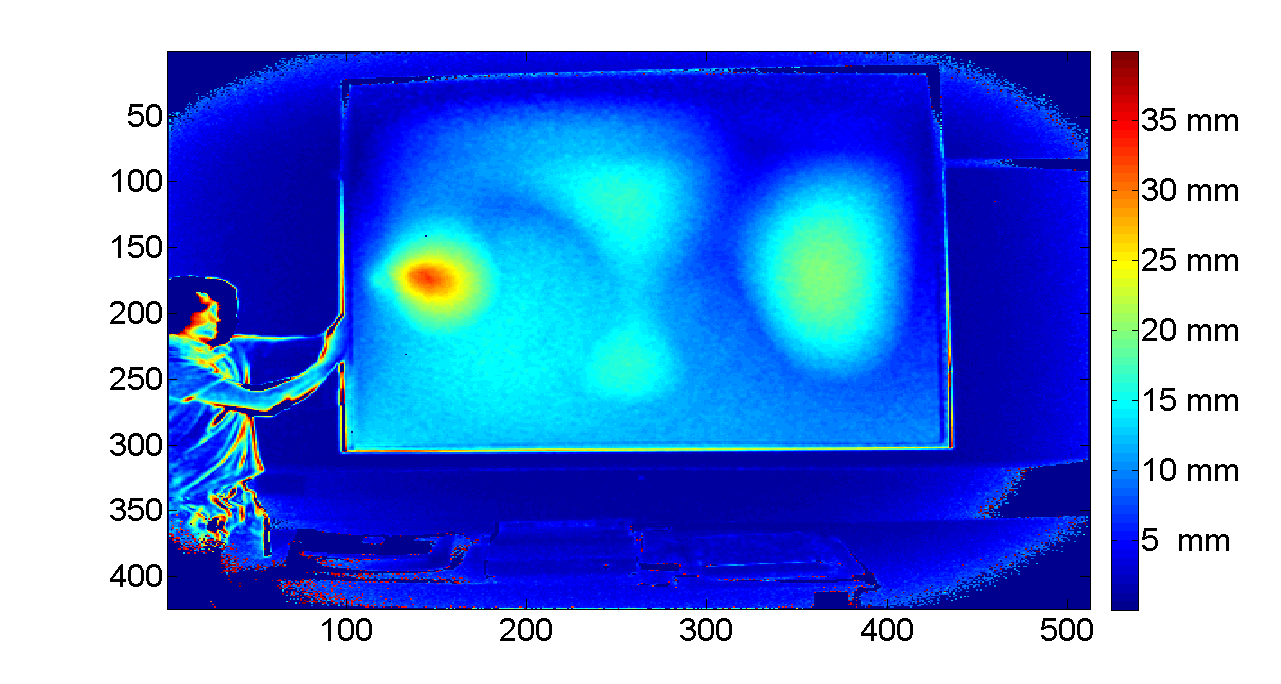
\includegraphics[width=0.9\textwidth]{Bilder/leinwand.png}
	\caption{Peak amplitudes of every pixel of a canvas excited by a person}
	\label{fig:Leinwand_FFT}
\end{figure}

For a better investigation of the image, a cursor can be used to investigate the dynamic of a single pixel or a pixel area. Figure \ref{fig:timedomain_leinwand} shows the time domain and figure \ref{fig:frequencydomain_leinwand} the frequency domain of a pixel in the region of the excitation. The highest peak indicates the dominating frequency $f_p\approx 4.8~Hz$ in the spectrum at an dominating amplitude $A_p\approx 15~mm$. The second peak at about $2.5~Hz$ results out of the offset of the signal. The first harmonic emerges at about $9.6~Hz$. Every periodic signal consists of the dominating frequency $f_p$ and its harmonics, which are integral multiples of the dominating frequency $f_p$. The strongest harmonic peak is indicated as $f_{ph}$ and $A_{ph}$.


\begin{figure}[!h]
	\centering
	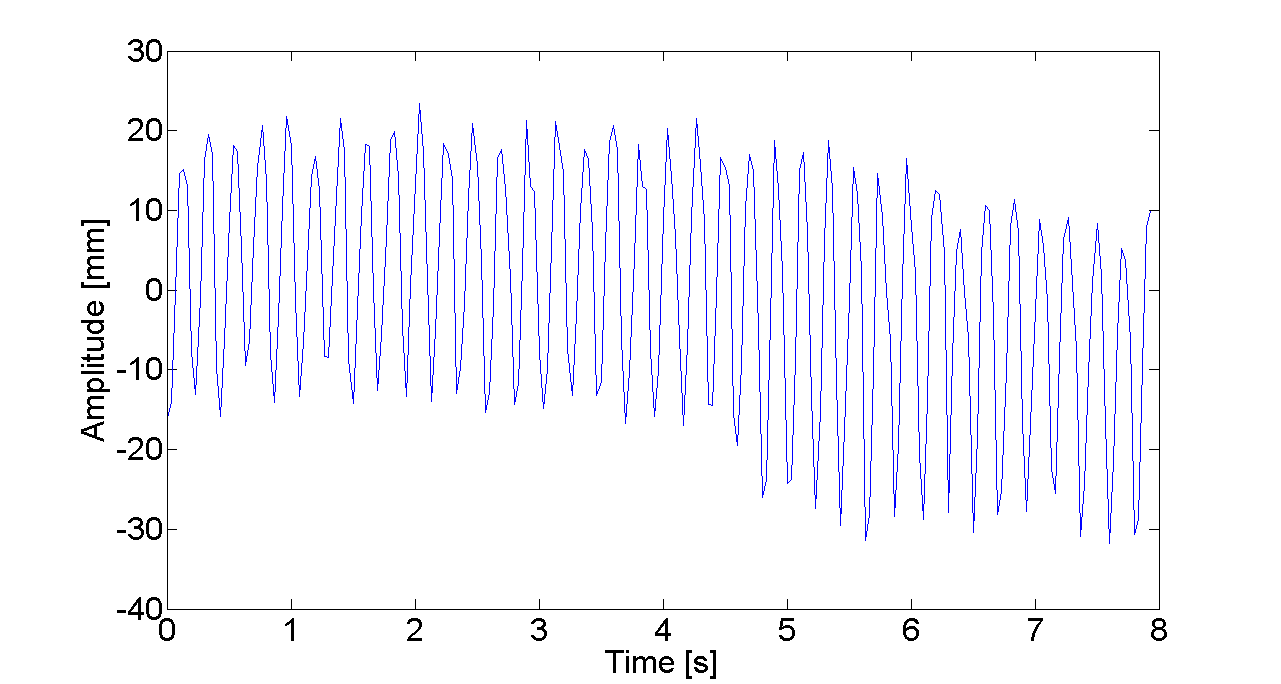
\includegraphics[width=0.8\textwidth]{Bilder/leinwandtimedomain.png}
	\caption{Time domain of excitation area}
	\label{fig:timedomain_leinwand}
\end{figure}

\begin{figure}[!h]
	\centering
	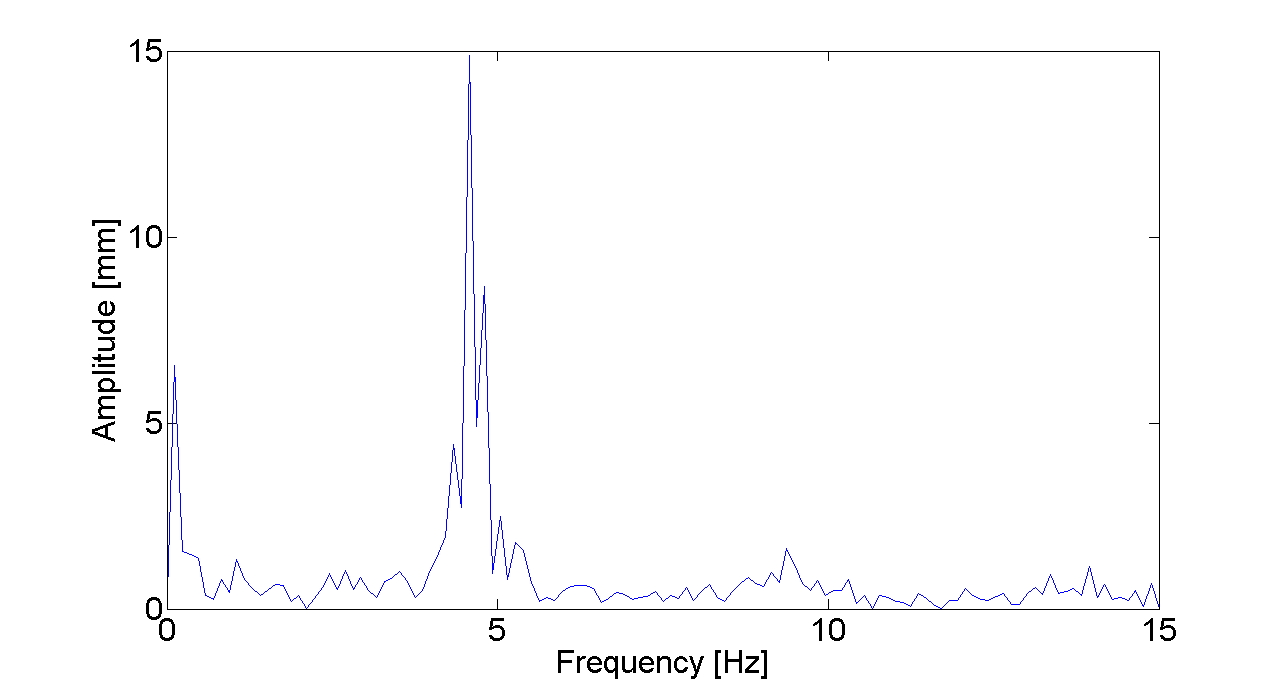
\includegraphics[width=0.8\textwidth]{Bilder/leinwandfrequencydomain.png}
	\caption{Frequency domain of excitation area}
	\label{fig:frequencydomain_leinwand}
\end{figure}

\newpage

\section{Data Processing of Laser Doppler Vibrometer} \label{chap:LDV_processing}
As an accurate and precise contactless measurement reference for the ToF camera, a Laser Doppler Vibrometer (LDV) runs parallel to the Kinect 2. The signal is transformed from fiber optic into a voltage signal, it is filtered and amplified before it is measured inside the Agilent DSO6054A oscilloscope. A digital interface delivers the access to the scope data. High sampling rates of common devices require a fast connection to gather the raw data over a long time. The digital resolution and sampling rate can also be reduced before it is transferred. Therefore, the data can be stored on a common USB stick in time domain CSV format. Columns are separated by comas and raws by new lines. This returns the time versus the voltage of every data point in two arrays of the same dimensions; Volt and Second. Equation \ref{eq:scope_capture} presents the way, how the reduced sampling rate is calculated depending on the TimePerDIV configuration on the screen, the number of samples $n_{samples}$ that are taken and the 10 rasters on the screen. TimePerDIV is adjusted by the knobs on the scope screen and $n_{samples}$ in the configurations.

\begin{equation}
\label{eq:scope_capture}
f_{sample}= \frac{n_{samples}-1}{TimePerDIV\cdot 10}
\end{equation}
\medskip

The time between every datapoint is the periode $T_{sample}$ and is used for the scaling of the time axis in the time domain and for the FFT analysis. 

\begin{equation}
\label{eq:sampling_period}
T_{sample}= \frac{1}{f_{sample}}
\end{equation}

For the transformation of the alternate voltage $U(t)$ in a corresponding speed $v$, the sensitivity $E$ adjusted at the LDV at the time of the measurement needs to be known. The CSV file format of the raw data can simply be imported in Matlab and transformed by equation \ref{eq:speed_transformation}.

\begin{equation}
\label{eq:speed_transformation}
v(t) = U(t) \cdot E
\end{equation}

 The direct current noise voltage needs to be removed from the data. This is done by a reduction of every value by the mean of all data. A better way would be to use a real high pass filer to remove the DC parts. The data needs to be integrated to get the displacement $z_{dyn(t)}$ from the speed v(t). The library offers a function cumtrapz() for this purpose. It computes an approximation of the cumulative integral via the trapezoidal method. The following source code extract shows the processing of the LDV data:

\begin{lstlisting} 
% Scope and Laser Doppler Vibrometer Data
E = 125 %%(mm/s)/V
n_samples = 1001; % zero based
TimePerDIV= 0.5 %s
f_samples = (n_samples-1)/(TimePerDIV*10);
speed =(Volt-mean(Volt))*E;
displacement=cumtrapz(speed)/f_samples; 
second=second+max(second);
\end{lstlisting} 

In the last step the time vector is corrected to start at zero. Afterwards, the displacement array can be processed in the same way as described in section Dynamic Analysis of Pixels \ref{sec:Dynamic_pixel}. The integration acts like a low pass filter. Sharp edges are removed and a smooth sinus remains. Equation \ref{eq:speed_sinus} shows the analytic mathematical integration of the speed to obtain the displacement. The constant offset $c$ must be calculated from other boundary conditions. This is helpful for a rough estimation of the displacement $z(t)$, directly at the scope with just the frequency $f$, sensitivity $E$ and the speed $v(t)$. The complete source code of the LDV data processing, which is done later in the experimental setup, can be found in the source code extract \ref{list:LDV_FFT}.

\begin{equation}
\label{eq:speed_sinus}
z(t)=\int v(t) dt = \int Asin(2\pi f t ) dt = -\frac{A}{2\pi f} cos(2\pi f t)  + c
\end{equation}


\begin{figure}[!h]
	\centering
	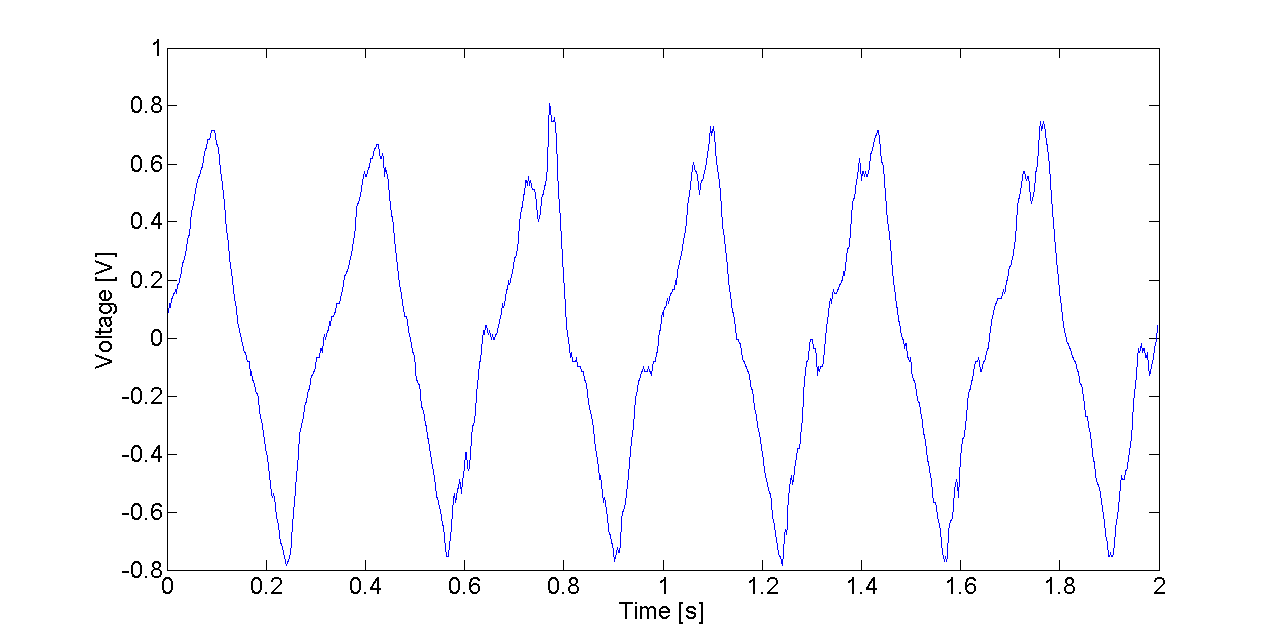
\includegraphics[width=0.7\textwidth]{Bilder/LDV_Row_data.png}
	\caption{$3~Hz$ Oscillating row data sampled with a scope}
	\label{fig:LDV_raw_Data}
\end{figure}

\newpage
%	Fazit und Ausblick
\section{Analysis of Depth Images} \label{sec:static_evaluation}
For a better understanding of the dynamic, the static behavior is analyzed in this section. The variance is the main dimension that will be investigated for that purpose. The static analysis is a measure for the noise floor. The variance should be as small as possible for a precise and accurate investigation of the dynamic investigation. It behaves as a disturbing dynamic that needs to be distinguished from the real dynamic. The analysis of absolute depth errors is not possible, since this requires a very precise experiment set-up. The positions must be adjusted over the complete range of $8~m$ in the resolution of the camera of $1~mm$. For a smaller range, this could be done on a lathe in the future. The following approaches shall give some rough estimations on the static behaviors. 

\subsection{Variance Depending on the Distance}   
The function of the variance $\sigma^2$ over different distances gives the fluctuation of a measurement in itself. As a consequence, the precision can be judged over the distance. Microsoft delivers its own measurement data of the standard derivation depending on the distance \cite{payne20147}. A direct comparison is not possible. The area that is kept fixed for the analysis is unknown. A translation between the variance $\sigma^2$ and the standard deviation $\sigma$ is possible by the following equation:

\begin{equation}
\sigma = \sqrt{\sigma^2}
\end{equation}

A white screen for overhead projectors with a very high diffuse reflectance of about $80\%$ has been captured over 3 seconds for the estimation of the variance. The investigated area is a 4x4 pixel window in the middle of the complete image. The area that is used for the dynamic investigations corresponds to this window. Therefore, the regions of the highest variance in the corners do not lie in the area. At the longest distance, the investigated area must still be completely on the screen. Afterwards, the mean variance of all pixels 16 is calculated in a time span of 3 seconds. The analysis has been done with the raw and TVD filtered data. As parameters for the filtering 20 iterations and $\lambda =1$ are used. The variance versus the distance is plotted additionally even if the measurement setup like the window size or the reflectivity is unknown \cite{payne20147}. 


\begin{figure}[!h]
	\centering
	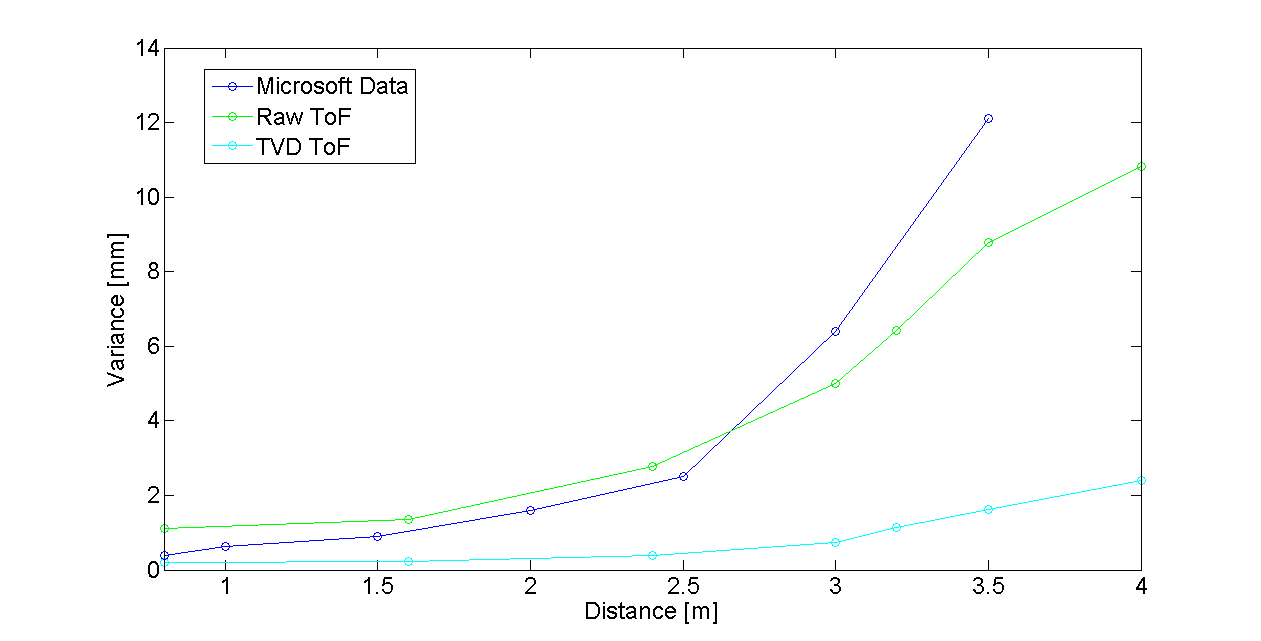
\includegraphics[width=0.8\textwidth]{Bilder/Var_vs_distance_MS.png}
	\caption{Variance vs. distance Microsoft data, raw and TVD after 3 Seconds}
	\label{fig:Variance_TVDvsRAW}
\end{figure}

The comparison between the raw and filtered data in figure \ref{fig:Variance_TVDvsRAW} shows a significant reduction in the variance over the complete distance with TVD. The raw data has a quadratic trend. This results out of the quadratic decrease of the light intensity versus the distance to the camera. The light propagates on sphere area into the room as shown in equation \ref{eq:solid_angles}. The noise increases and the signal decreases with higher distances that correspond to a lower SNR. 

\subsection{Variance Depending on Geometries and Surfaces}
A simple way to investigate the variance difference between high reflecting white and low reflecting black surfaces is possible on a checkerboard. Squares of the same size on a flat surface are easy to distinguish with different reflectivity properties even if they lie on the same surface. This is also a common approach to calibrate the distortion of a standard camera objective. Figure \ref{fig:checkerboard} illustrates the change of the variance between the black and white areas in a one meter distance after a recording time of $3~s$. The black fields feature a higher variance than the white ones. The sticker material of the checkerboard has spread reflection characteristics. Therefore in the middle of the image more light is reflected backwards into to the sensor than on the outer areas. The variance in the middle is reduced. More light is reflected backwards. A calibration of the Kinect 2 is not necessary since the focal lens is fixed and the correction of the distortion is done in the image processing of the camera. 
The reflection characteristics on various material does not always behave in the same way as for visible light. This is shown on some random objects measured in there variance for a rough estimation between different surfaces. In figure \ref{fig:Material_Investigation}, a collection of geometries and surfaces are investigated. Except for the black flat plastic with a thick layer of clear paint and the polished aluminum pipe, all material probes show a low variance. The black plastic absorbs and spectral reflects most of the IR light and the pipe scatters the light in a spectral way to all sides. Only the middle part of the pipe parallel to the image plane is of low variance. More light is reflected backwards. Even if the heck spoiler and the copper sheet are spectral reflecting for visible light, this is not the case in the IR spectrum.\\ 

Flying pixels cause a high variance at the boarder of all objects. To distinguish small changes in the color space, larger variance values than $140~mm$ and distances behind the objects are set to zero. The influence of the angle to a plane surface has not been investigated. The change of variance on different geometries and surfaces should be part of further investigations. 

\begin{figure}[!h]
	\centering
	\includegraphics[width=0.77\textwidth]{Bilder/checkerboard.png}
	\caption{Variance on a checkerboard in $1~m$ distance}
	\label{fig:checkerboard}
\end{figure}

\begin{figure}[!h]
	\centering
	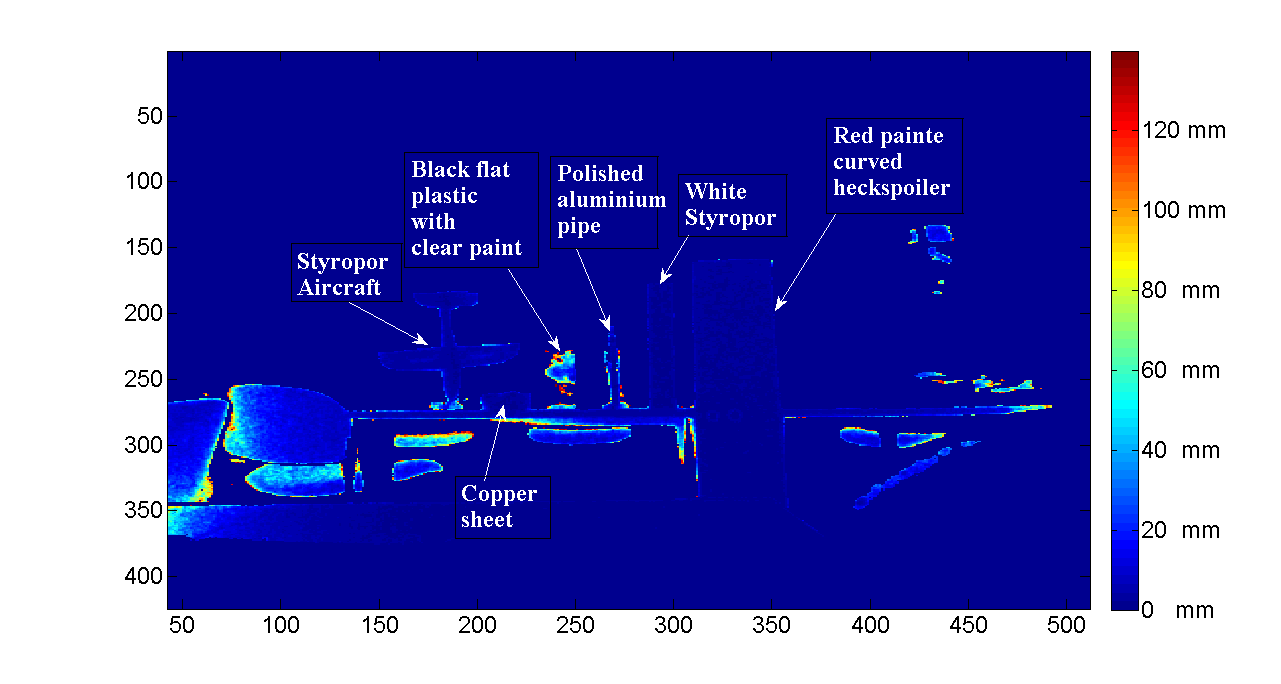
\includegraphics[width=0.77\textwidth]{Bilder/Material_Investigation.png}
	\caption{Variance on various geometries and surfaces}
	\label{fig:Material_Investigation}
\end{figure}

\subsection{Influence of Background Lighting on Static Measurements} \label{chap:static_Lighting}
The variance of the static bass membrane plays an impotent role for further dynamic analysis. A reduction in the noise characteristic is done with 5 white matt paper stickers attached to the membrane. This gives a clear sharp boarder to the original black surface. 2000 W of halogen light are pointed on the membrane to disturb the measurement from the position of the camera by a second IR light source. This data is compared with a recording in absolute darkness. The position and $1.4~m$ distance of the camera to the membrane are unchanged. The distribution of variances is illustrated in figure \ref{fig:membrane_static_dark} for the dark and in figure \ref{fig:membrane_static_halogen} under halogen lighting. The depth data of the background behind the membrane is set to zero. The light impact is remarkable on the black cone surface. The white paper is influenced much less by the IR lighting. The reason for that is the low SNR on the black cone. The IR light of the ToF measurement is strongly absorbed and scattered on this surfaces. With the IR impact of the halogen lighting, the noise is additionally increased to values higher than $500~mm$. This is caused by a spread spectral reflection, which directs a high amount of IR halogen light directly into the camera. The RGB image of the Kinect in figure \ref{fig:KinectScreenshot-Color-10-58-52} shows the same saturation caused by the spread reflection.

\begin{figure}[!h]
\subfigure[Variance on the static membrane in a dark room]{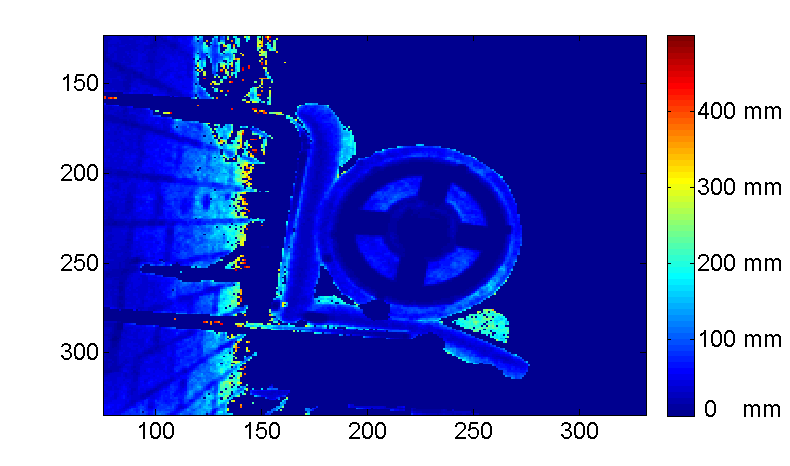
\includegraphics[width=0.5\textwidth]{Bilder/membrane_static_dark}\label{fig:membrane_static_dark}}\hfill
\subfigure[Variance on the static membrane and $2~kW$ halogen]{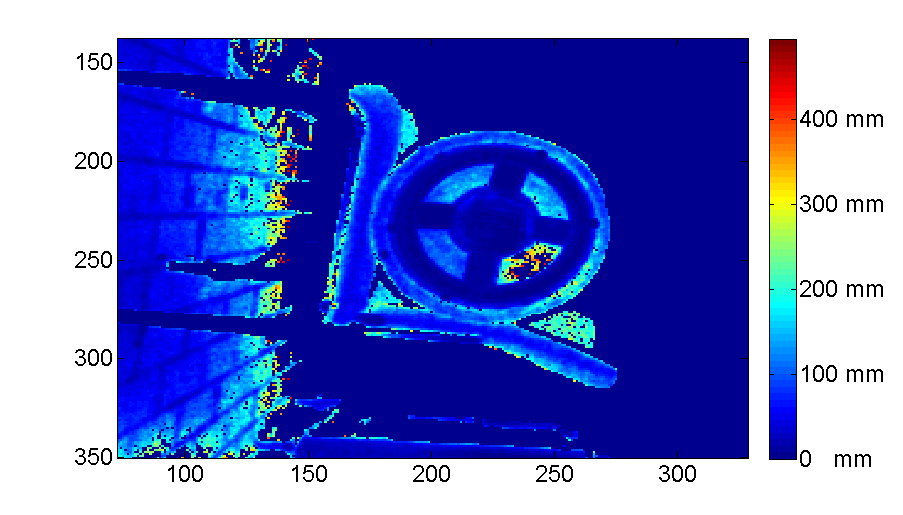
\includegraphics[width=0.5\textwidth]{Bilder/membrane_static_halogen.png}\label{fig:membrane_static_halogen}}
\centering
\caption{Influence of halogen lighting on the variance}
\end{figure}
 
\section{Evaluation of Membrane Dynamic} 
\subsection{Physical Model of Membrane Oscillation and Observation} \label{sec:bias_membrane}
This section delivers a physical model for the vibration of a subwoofer membrane in the investigated low frequency area $f_{ref} \leq 10~Hz$. Due to the low frequency excitation, every point moves with the same speed $\vec{v}(t)$ and the same phase into the normal direction $\vec{n}$ of the middle flat surface.  The measurement of the vibration under a bias angle is characterized by the angle between the optical axis and the surface normal, called viewing angle $\alpha$. Since LDV measures only the speed into the direction of the optical axis, the amplitude $A_{LDV}$ is reduced under higher angles to the surface normal. Figure \ref{fig:membrane_geometry} illustrates the basic geometries of the membrane observation. The viewing angle $\alpha$ is defined between the surface normal $\vec{n}$ and the optical axis turning into the negative mathematical direction. In contrast to that, the ToF amplitude $A_{ToF}$ is increased by the bias observation since the investigated pixels are moving sideways and ToF delivers the absolute distance and not a relative speed like LDV. With a cone angle $\beta$, the oblique areas delivers different normal surface angles and therefore $\alpha$ is changed. This physical model shows the relationship between the viewing angle $\alpha$ and the resulting amplitude of $A_{LDV}$ and $A_{ToF}$ represented by equation \ref{eq:tof_amplitude} and \ref{eq:ldv_amplitude}. This model assumes that the ToF camera has an infinite numbers of pixel. In practice this is not fulfilled. One pixel will therefore cover multiple distances under high angles. On the upper and lower surfaces the angle $\alpha_{l,u}$ depends on the oblique position of the cone surface and the angle $\beta$ to the middle surface. The coordinate system of the membrane is represented by the index (m) and has the same orientation as the scene plane coordinate system that is given by the depth images.  
  
\begin{equation}
A_{ToF} = A_m (\cos \alpha +1)
\label{eq:tof_amplitude}
\end{equation}

\begin{equation}
A_{LDV} = A_m \cdot \sin \alpha 
\label{eq:ldv_amplitude}
\end{equation}
 
\begin{equation}
\alpha_{l,u} = \alpha \pm \beta
\label{eq:alu_angle}
\end{equation}
\newpage

\begin{figure}[!h]
	\centering
	\includegraphics[width=0.8\textwidth]{Bilder/Geoemtry_membrane_amplitude.pdf}
	\caption{Geometry of bias membrane observation}
	\label{fig:membrane_geometry}
\end{figure} 

\bigskip
\begin{figure}[!h]
	\centering
	\includegraphics[width=0.9\textwidth]{Bilder/displacement_timedomain_membrane.png}
	\caption{Displacement of the membrane measured on the middle surface with a Laser Dopper Vibrometer under $\alpha = 0^\circ$}
	\label{fig:displacement_timedomain_membrane}
\end{figure} 

\newpage


\subsection{Scientific Problem} 
The dynamic behavior of a membrane is the test body for a detailed analysis of the ToF principle for dynamic measurement of surface vibrations. The membrane is excited and acquired under variable conditions to investigate multiple scenarios. A bass tube is plugged to a waveform generator, creating a defined vibration that is recovered from multiple ToF 3D scans. This data is compared with a Laser Doppler Vibrometer (LDV) as a reference. LDV delivers the accurate data of a single point on the membrane, whereas ToF measures the complete surface movement. Multiple questions will arise from that: One is the precision and accuracy distribution in frequency and amplitude over the membrane under different conditions. Which part cannot be investigated and which area is overlaid by noise? The influence of angle, distance, frequency and amplitude is questioned. How is the measurement influenced by an additional IR light source that emits in the same spectrum as the ToF laser diodes? Another questions is the influence of static filter method for the dynamic investigation. Is a reduction of the noise possible without an impact on the actual dynamic? Is the complete signal-to-noise-ratio influenced by the filtering? Can overtones like the first or second harmonic still be derived from the ToF data? How does ToF behave in a continuous change in frequency and amplitude? ToF allows the investigation of the complete field of view. How can the dynamic of a surface be illustrated? The following section tries to investigate all these questions in detail. The membrane movement should deliver an ideal test body, because it vibrates in only one direction at a stable frequency and amplitude. The vibration is controllable in frequency and amplitude. This approach could later be useful for the calibration of ToF for vibrations measurements with a scientific camera and under more controlled conditions. The experimental setup shall deliver first steps into this direction, showing the performance of ToF and, how the data can be processed in Matlab.   

\subsection{Hypothesis}  
With the depth resolution of $1~mm$ and a variance lower than $1.2~mm$ up to a distance of $2~m$, the system should be capable to distinguish changes of amplitude in the magnitude of the $1~mm$ depth resolution. Except for the corner of the images, a dynamic investigation in the whole field of view should be possible for distances blow $2.5~m$, because the variance in this distance is below or in the region of the depth resolution. Processed by a Fast-Fourier Transform, a vibration with a amplitude higher than $1~mm$ should always return the strongest peak in the frequency spectrum. With a sampling rate of $30~fps$ and an maximum vibration frequency of $10~Hz$, the limits of the Nyquist-Shannon theorem for dynamic measurements are satisfied. A precise determination in frequency should be possible on all areas of the membrane. An oversampling factor of 5 should be enough for the reconstruction of the wave form and amplitude. Therefore, every sinus period is sensed by 10 samples. Consequently, a precise reconstruction of a $3~Hz$ should be possible in frequency and amplitude. The change of the viewing angle $\alpha$ influences the amplitudes magnitude into the direction of the ToF camera and the SNR. The ideal trend should follow the physical model that is represented in section \ref{sec:bias_membrane}. The displacement of ToF is increased with higher viewing angles and the low reflection backwards to the sensor will cause a high inhomogeneous in the amplitude distribution. Single points of the membrane do not correspond to single pixels in the depth image any more. The impact of the filter method depends on the amplitude and the parameter of the filtering. A high smoothing of the image pixels should not just decrease the variance but also the vibration's amplitude. The impact of black versus white surfaces should be significant in the dynamic analysis. Figure \ref{fig:membrane_static_dark} already implies, that the black oblique parts have a higher variance, overlying the vibration. The influence of a second IR light source should decrease the SNR ratio and therefore also the accuracy of the measurement.\\ 

Amplitudes higher than $1~mm$ with lower frequencies than $10~Hz$ will emerge in a Short-time Fourier transform. The resulting spectrogram should deliver a simple and detailed way to investigate multiple frequencies with ToF and LDV in a single signal.\\

By extracting maximum values out of every pixel's FFT, the frequency and amplitude distribution can simply be illustrated. Differences in the surface's dynamic are recognizable. The distribution of the first and second harmonics will be visible even on high reflecting surfaces with a low SNR. 
  
\subsection{Measurement Setup}
  
The direct comparison between ToF and LDV requires the measurement from preferably the same point and the same distance to the vibration. Since this is not possible, both devices are mounted together on a single tripod. The direction of the perspective should be as close as possible to avoid bias differences in the viewing angle $\alpha$. The LDV is mounted near the IR camera of the Kinect 2 device. Figure \ref{fig:ToF_LDV_Team} shows the assembly of both devices. The LDV should never point into eye-height to avoid hazard of the human eye. The experiment is performed in an dark room without windows and just two halogen lights at the ceiling. The Kinect 2 images are recorded by a desktop PC via an USB 3.0 connection. The open source software dumpK4W was used for the recording of the "raw" images. It saves every image from the video stream into an uncompressed tiff image. The depth information in every pixel is already represented in millimeter dimensions. Thereby, a calibration is not necessary. The USB 3.0 controllers require a high data throughput. Some older USB 3.0 chipsets are overcharged by the high data stream from the two cameras and the three microphones. Microsoft delivers a list of chipsets which are capable to handle that. The data stream is captured for 3 or 8 seconds. Before an import into Matlab is possible, all other images like RGB have to be removed by hand. The acquisition has to be repeated, if the number of images does not fit to the capture time. Running a D2D example program with a live video stream at the same time reduces the number of lost images. The Polytec CLV700 is the LDV that is used as a reference device. An optical fiber connection delivers the high monochromatic laser beam to the sensor head. From there, the laser beam radiates on the surface and reflects backwards into the sensor head. The resulting interfering light is transported backwards into the analog input module CLV-M200 for the evaluation. The decoder module CLV-M030 amplifies the voltage to a adjustable range. 125 $\frac{mm}{s}/V$ is configured in this stage by a knob. A lower value was not possible since the high amplitudes of the membrane lead to a saturation in the decoder module. Up to $1.250~mm/s$ can be measured in this configuration at resolution of $2~\mu m/s$ \cite{CLVpolytec}. The BNC connection delivers the analog signal to the oscilloscope, that is necessary to sample the high voltages up to $10~V$. With the Agilent DSO6054A Digital Oscilloscope, the analog signal is sampled depending on the configuration shown in section \ref{chap:LDV_processing}. Only the TimePerDIV parameter of the screen and the $n_{samples}$ influences the way the data is acquired. The compressed data is saved on the USB Stick in the CSV file format. This has to be configured inside the print options. Matlab provides pre-built functions for the automatic input of the CSV formated data.  Since the frequencies of the input signal $f_{ref}$ are lower than $10~Hz$, the oscilloscope is not able to trigger the screen on the input signal. The refreshing of the screen occurs in free-run operation. 
The membrane in the subwoofer tube is driven by a $240~W$ Yamaha A-S500 integrated amplifier in pure direct mode without any filtering. The inner part of the membrane should be as flat a possible. Consequently, ToF and LDV have a uniform plane surface that can be investigated for deformations. The tube is located on a chair at the height of the LDV and TOF perspective. The Agilent Waveform Generator 33120A creates the audio signal that is feet into the amplifier on a mono line by a self made BNC to chinch cabel. Before a direct connection is established, the output voltage is checked to match the standard line level criteria. Levels above $U_{pp}=3.472~V$ for professional equipment and $U_{pp}=0.894~V$ for consumer equipment can damage the electronic. The line level is an alternating current signal without a direct current offset. A standard audio output, that is measured with the scope, should deliver the same $U_{pp}$ value at the maximum volume. All measurement devices that are connected to each other are plugged together in one mains socket to avoid ground loops and therefore interference between devices like $50~Hz$ noise. For a higher reflectivity of the ToF IR light, white paper stickers are attached to the flat surface and the oblique outer parts. It should feature a high paper density to achieve a reflectance $\varrho$ of 80 $\%$ and higher. The middle sticker has a dimension of $76x39~mm$. The LDV requires a small reflecting tape on the inner surface to increase the intensity of the reflected laser beam as seen in figure \ref{fig:membrane}. Figure \ref{fig:experimental_setup} narrows the experimental setup down to the important components. The distance and angle to the membrane is illustrated. The reconfiguration of this parameters is done in a roughly way with a common measuring tape and a radian measure. 
\bigskip
\begin{figure}[!h]   
	\centering
	\includegraphics[width=1.0\textwidth]{Bilder/Experimental_setup_Final_1711.pdf}
	\caption{Sketch of the experimental setup}
	\label{fig:experimental_setup} 
\end{figure}     

\begin{center}
	\begin{tabular}{| l | l | l |}
		\hline
		\textbf{Device} & \textbf{Information} & \textbf{Configuration} \\ \hline
		Polytec CLV700 & HeNe Laser Safety II  & Variable laser focus   \\ \hline
		Input Module CLV-M200 & $v_{max}=1.250~mm/s$ & $2~\mu m$ Resolution  \\ \hline
		Decoder Module CLV-M030 & Resolution = $ 2~\mu m/s$ & $125~mm/s/V$  \\ \hline
		Output Module CLV-M001 & - & $5~kHz$ Low-pass filter \\ \hline
		Kinect 2 & $512x424~30$ fps & Depth resolution $1~mm$ \\ \hline
		Agilent 33120A Waveform Generator  & Uncalibrated & $0.894~V_{pp}$ \\ \hline
		Agilent DSO6054A Oscilloskop & $500~MHz$ & $1000, 500~or~250~ms~per~DIV$ \\ \hline
		Yamaha A-S500 Amplifier & $150~W$ Mono & pure direct / no filtering \\ \hline
		Matlab R2013a & - & - \\ \hline
		Subwoofer & 30'' JBL Car Tube & Paper Sticker / Reflector \\
		\hline 
	\end{tabular} \captionof{table}{Devices of experimental setup}	
\end{center}

\begin{figure}[!h]
	\centering
	\fbox{\includegraphics[width=1\textwidth]{Bilder/Versuchsaufsbau_TOF_LDV.jpg}}
	\caption{Experimental setup}
	\label{fig:ToF_LDV_Team}
\end{figure} 

\newpage
\begin{figure}[!h]
	\centering
	\fbox{\includegraphics[width=1\textwidth]{Bilder/Kinect_2_LDV_Team.jpg}}
	\caption{LDV and Kinect 2 mounted on one tripot}
	\label{fig:ToF_LDV_Team}
\end{figure} 

\begin{figure}[!h]
	\centering
	\fbox{\includegraphics[width=1\textwidth]{Bilder/Membrane_laser.jpg}}
	\caption{Membrane with white paper stickers and reflector}
	\label{fig:membrane}
\end{figure} 

\newpage

\subsection{Test Procedure}
Some fundamental boundary conditions apply for all experiments that are done. Every device should be turned on for some minutes before the execution to achieve a stable temperature. ToF cameras are in general sensitive in their accuracy for fluctuation in temperature \cite{foix2011lock}. The IR lighting and electronic heats up the device over time. The LDV is pointed together with the ToF camera on the membrane with reflector and the white paper attached to it. The membrane is in the middle of the field of view in the distance d and the viewing angle $\alpha$ to the normal vector $\vec{n}$ of plane middle surface. If no angle is given, it is kept constant at $\alpha = 0^\circ$. The LDV signal indicator should be at least at a level of about $30~\%$ to guaranty a high SNR. Afterwards, the volume of the amplifier can carefully be turned up. Ideally, no sound should be hearable with frequencies lower than $30~Hz$. In practice, the membrane creates noise in higher frequencies even if it excited in the 1 to 10 Hz range. The LDV is capable to measure this sounds as spikes on the sinus oscillation. It is a sign for an overdrive of the subwoofer. The high amplitudes can cause the membrane to detach from the tube. The attachment is checked under the highest amplitude and frequency according to equation \ref{eq:Energy_oscillation}. The tube and the structure itself should not get excited. The peak-to-peak value is displayed on the oscilloscope and should stay in a narrow band. It is an indicator for a stable oscillation at a constant amplitude \ref{chap:LDV_processing}. Every measurement point is the mean from a 4x4 pixel window that is chosen by the user as near a possible to the LDV measurement at the middle of the white paper. Since the laser reflector is also spectral reflecting the ToF IR lighting, an investigation of the same point is not possible. The reflector leads to a hole in the 3D scan. Some safety guidance for humans, environment and devices have to be kept in mind. The laser beam should never be attached in the height of the human eye to avoid damages to the retinal after long exposure. The membrane is another source of danger. High amplitudes up to $10~mm$ require the volume to be turned up to a maximum. The same volume in the audible range can damage the eardrum. So a change in frequency at the waveform generator has to be done with caution. Structures in the environment of the test are also exposed by the strong vibrations and can be excited in there eigenfrequencies. The influence of background lighting is characterized in a distance of $1.4~m$ at $3~Hz$ with $2000~W$ halogen lighting at the position of the cameras pointing on the membrane. An RGB image from the Kinect's perspective is visible in figure \ref{fig:KinectScreenshot-Color-10-58-52}\\

The data is captured in a unsynchronized way. This means, that single data points cannot be compared to each other. It is only possible to analyze single deflections to each other in the variable displacement setup. In all other configurations it is assumed, that the oscillations is kept stable over the complete acquisition time. In this way, small time delays between the ToF and LDV measurement have a small impact on the results in the frequency domain. Nevertheless a time synchronization is beneficial. Both measurements must take place in the same time span. The acquisition of both devices is started manually. At first, by the commandline on the PC to start ToF and afterwards by pressing the "Quick Print" button on the oscilloscope to acquire the LDV data. Since low frequencies can not trigger the screen, the measurement should be started when the signal trend ends at the right side of the screen.    

\subsubsection{Variable Distance}
The first parameter being changed, is the distance d of the tripot to the middle of the membrane. A high precision horizontal movement is not possible with the given equipment. The rough estimation is done with a measuring tabe. The $0^\circ$ viewing angle of the laser beam to the surface normal vector should be kept constant under all conditions. The volume and the frequency of the waveform generator $f_{ref}=3~Hz$ is unchanged for all measurement points. The  amplitude of about $4~mm$ is high enough to distinguish it from noise under the maximum distance. For every measurement point the focus of the LDV has to be readjusted to a sufficient signal level. The noise is reconsidered for every distance and can be minimized by gently moving the sensor head. The first run of the experiment is done for 3 seconds of ToF and 2 seconds of LDV. The second run will be done for 10 seconds of LDV and 8 seconds of ToF. At a distance of $1.4~m$ the setup is added with $2000~W$ of halogen lighting at the position of the camera to disturb the ToF measurement on the membrane with additional IR light.

\subsubsection{Variable Angle}   
Since there is no precise setup for the viewing angle $\alpha$ determination, it is estimated by a goniometer on the floor. In the distance of $1.4~m$ and $2.0~m$ the angle $\alpha$ is changed from $90^\circ$ to $0^\circ$ in $5^\circ$ steps at a constant frequency of $f_{ref}=3~Hz$. $\alpha$ is the angle between the optical axis of the camera and the  middle surface turning in the mathematical positive direction. The focus must be readjusted for every angle. It is ensured, that the laser points on the reflector over the complete displacement of the membrane at every angle. The area of the LDV and ToF measurement is therefore increased with higher angles. The simplest way to change the angle between the perspective and the membrane is by turning the subwoofer on the measurement point. The paper stickers are compared with each other. The one in the middle delivers a surface under the angle $\alpha$. The lower sticker has an angle of $\alpha + 38^\circ$ and the lower of $\alpha -38^\circ$ due to the cone. 

\subsubsection{Variable Frequency}
The change of frequency from $10~Hz$ to $1~Hz$ is done in a distance of $1.4~m$ at a constant volume in one $1~Hz$ steps at $\alpha = 0^\circ$ to the surface normal. Since the frequency change at the functions generator cannot be separated from a change in the maximum displacement, the amplitude cannot be kept constant for different configurations. The membrane should still be out the overdrive region to archive comparable data, at the highest frequency. The acquisition takes place at every parameter for 8 seconds to capture enough periods at the lower frequencies.     

\subsubsection{Variable Displacement}
The volume is turned up from $0~\%$ slowly for a brief moment and reduced afterwards for the investigation of different displacement of the membrane. This configuration can also be considered as an amplitude sweep, because the volume is changed during the data recording. Only a small number of oscillations is analyzed and can be compared with the idle state before and after the oscillation. The acquisition takes place for 8 second to allow enough time for turning the volume up and down manually. 

\subsubsection{Sweep}
The adjustment of the frequency versus time is called Sweep. At a constant volume, the frequency is increased manually in $0.1~Hz$ steps from $1$ to $10~Hz$. Ideally, this is done automatically by the function generator in a smaller resolution. The measurement takes place over 10 seconds with ToF and LDV. To gather all the date with the scope in this time span, $f_{sampling}$ has to be decrease to $100~Hz$. No noise should occur at the highest frequency in order to avoid deviations of the ideal sinus trend. 

\newpage

\subsection{Measurement Results}
All data is processed by the $dynKinect\_0\_3\_thesis\_evaluation.m$ Matlab script. The TimePerDIV parameter is the only number that has to be chosen manually depending on the acquisition time of the oscilloscope. From this $f_{sampling}$ results according to equation \ref{eq:scope_capture}. The wrong parameter will change the amplitudes, times and frequencies in the domains. For a comparison between the devices, raw data is transformed into the frequency domain by the fft() function shown in chapter \ref{sec:Dynamic_pixel}, \ref{chap:LDV_processing} and \ref{chap:frequency_domain}. The Short-time Fourier transform method is used for the sweep analysis. In the frequency domain, noise and dynamic are easy to separate. The strongest peak in a 4x4 pixel windows is the value that is compared and plotted versus the change of parameters. In a distance of $2.6~m$, the window still fits on the sticker of $76x39~mm$ according to equation \ref{eq:pixel_area} and figure \ref{fig:area_of_4x4_pixelwindow}. Every data point is written into a CSV file by hand. The file is shifted into the Matlab workspace afterwards. A small script called $xy\_plotter.m$ is used to plot the data into graphs automatically.

\newpage

\subsubsection{Variable Distance}

Figure \ref{fig:Distance_vs_Amp} shows the progress of a the raw and TVD filtered data versus the reference LDV measurement after 3 seconds. LDV delivers two distortions at $1.1~m$ and at $1.8~m$ that cannot be explained by the instability of the membrane. A detailed analysis in the time domain shows an error in the processing with Matlab. Plotting clarifies an unsteady trend. This behavior is not noticeable in the raw data of the oscilloscope. Equally to the $1.8~m$ position, a strong jump of about $3~mm$ can be observed in the frequency and time domain additionally. A second peak near $0~Hz$ appears in the time domain and is a measure for the offset. Such behavior cannot be observed in the ToF data. A reason for that could be noise in the LDV measurement or an incorrect integration procedure. That is why those two points are not used as a reference and not plotted in the LDV data. Apart from that, the amplitude is reconstructed with a maximum error of about $1~mm$ by ToF. The membrane works stable in a range of about $0.4~mm$ in all distances at around $3.5~mm$ amplitude according to LDV. An influence of the distance on the accuracy is not clearly visible. The TVD filter could increase the accuracy in the distance between $0.9~m$ and $1.6~m$ with fixed parameters. Strong distortions like in $1.3~m$ and $1.6~m$ are reduced. In other distances, the filtering reduces the accuracy in contrast. Figure \ref{fig:0_6m_to2_6m_3Hz_240frames} visualizes the influence of a longer acquisition time of LDV and ToF in a second series of tests. The amplitude is reconstructed by LDV in smaller range of about $0.2~mm$ with no distortions. ToF delivers a strong deviation at $0.8~m$. The reason for that could be light scattering between the sensor and the lens. Too much light is reflected from the white paper surface. Apart from that point, the amplitude is reconstructed in a band of about $0.7~mm$. In the distance of $1.3~m$ to $1.5~m$, the absolute error is minimized down to a value of $0.05~mm$. The increased acquisition time allows a better separation of the variance from the actual dynamic. Figure \ref{fig:area_of_4x4_pixelwindow} delivers the projected area of the 4x4 pixel window versus the distance at a viewing angle of $0^\circ$.

 \begin{figure}[!h]  
 	\centering
 	\includegraphics[width=0.63\textwidth]{Bilder/area_of_4x4_pixelwindow.png}
 	\caption{Theoretical area of 4x4 pixel window versus distance}
 	\label{fig:area_of_4x4_pixelwindow}
 \end{figure}        

\begin{figure}[!h]  
	\centering
	\includegraphics[width=0.95\textwidth]{Bilder/Distance_vs_Amp.png}
	\caption{Amplitude $A_p$ versus distance after 3 seconds of ToF measurement}
	\label{fig:Distance_vs_Amp}
\end{figure} 

\begin{figure}[!h]  
	\centering
	\includegraphics[width=0.95\textwidth]{Bilder/0_6m_to2_6m_3Hz_240frames.png}
	\caption{Amplitude $A_p$ versus distance after 8 seconds of ToF measurement}
	\label{fig:0_6m_to2_6m_3Hz_240frames}
\end{figure} 

A direct comparison of the time domain data of ToF in figure \ref{fig:Time_domain_ToF} and LDV in figure \ref{fig:Time_domain_LDV} shows the huge difference in the sampling rate and resolution. The digital resolution of $T_{sample} = 33.3~ms$ in time and $1~mm$ in depth is noticeable in the ToF data. Regions of high acceleration at the peaks of the displacements have sharp digital edges in the sinus trend. This leads to additional fluctuations in the peak values. The LDV data proves the high short time stability of the membrane vibration. The short spacing in time of $T_{sample} = 5~ms$ and in displacement of $2~\mu m$ very precisely reconstructs the trends. A better comparison between a set of ToF and LDV data can be done in the frequency domain after a FFT. Figure \ref{fig:Freq_domain_ToF} and \ref{fig:Freq_domain_LDV} shows the ToF and LDV in the frequency domain in $1.4~m$ distance. The difference in the amplitude $A_p$ is $0.063~mm$ and in frequency $0.117~Hz$. The obvious error in frequency can be explained by the digital resolution in time of $T_{sample}=0.033~s$. Even the first and second harmonic component are clearly defined and match to the spectrum of LDV. On other parts of the membrane, the harmonics cannot be distinguished from noise that clearly as on the oblique black cone surfaces. Figure \ref{fig:Freq_domain_ToF_2m}  and \ref{fig:Freq_domain_LDV_2m} illustrate the frequency domain in $2~m$ distance. The first and second harmonic can still be seen in the ToF spectrum. The error of the absolute peak is increased to $+0.402~mm$. In the LDV data, the third harmonic is still visible. An offset peak at $0.1953~Hz$ of $0.3618~mm$ appears in the LDV data but not in the ToF data. 

\begin{figure}[!h]  
	\centering
	\includegraphics[width=0.80\textwidth]{Bilder/Time_domain_ToF.png}
	\caption{Time domain of ToF after $8~s$ in $1.4~m$ distance}
	\label{fig:Time_domain_ToF}
\end{figure}  

\begin{figure}[!h]  
	\centering
	\includegraphics[width=0.78\textwidth]{Bilder/Time_domain_LDV.png}
	\caption{Time domain of LDV after $8~s$ in $1.4~m$ distance}
	\label{fig:Time_domain_LDV}
\end{figure}  

\newpage
For a detailed illustration of complete surface dynamics, two new images are created from the $1.0~m$ data. Every pixel of the ToF video stream is analyzed in the FFT and a new image is plotted depending on the highest peak $A_p$ in the spectrum. Section \ref{sec:Dynamic_pixel} explains the creation of such images more detailed. The challenge is to integrate the frequency or the amplitude into a 2D plot in a huge range with a high contrast in the colorspace. The dynamic information from the video data is transferred into a single image. Figure \ref{fig:Freq_distribution} illustrates the dominating frequency distribution of $f_p$ on the membrane. Most pixels measure the correct $3~Hz$ frequency. Some areas on black oblique surfaces are dominated by noise of a random spectrum. The frequencies are shifted slightly. At the edges of the stickers, the amplitudes and frequencies are highly increased. An explanation is the a fluctuation of variance between the white and black field in the area that is observed by the pixel. The change in variance overestimates the actual defection.\
\begin{figure}[!h]
	\subfigure[ToF Frequency Domain]{\includegraphics[width=0.5\textwidth]{Bilder/Freq_domain_ToF.png}\label{fig:Freq_domain_ToF}}\hfill
	\subfigure[LDV Frequency Domain ]{\includegraphics[width=0.5\textwidth]{Bilder/Freq_domain_LDV.png}\label{fig:Freq_domain_LDV}}
	\caption{$3~Hz$ excitation in $1.4~m$ distance}
\end{figure}

\begin{figure}[!h]
	\subfigure[ToF Frequency Domain]{\includegraphics[width=0.5\textwidth]{Bilder/Freq_domain_ToF_2m.png}\label{fig:Freq_domain_ToF_2m}}\hfill
	\subfigure[LDV Frequency Domain ]{\includegraphics[width=0.5\textwidth]{Bilder/Freq_domain_LDV_2m.png}\label{fig:Freq_domain_LDV_2m}}
	\caption{$3~Hz$ excitation in $2.0~m$ distance}
\end{figure}
\newpage
 Another abnormality is given by the LDV reflector. The IR light is reflected spectral on this surface. A depth measurement is not possible here and therefore also no dynamic investigation. The static surfaces around the membrane illustrates this in chaotic colors. The dominating frequencies on the static surfaces depend on the variance that shows a very high entropy. Figure \ref{fig:Amp_distribution} clarifies the amplitude distribution. Higher values than $5~mm$ are removed to distinguish small changes in the colorspace. The white paper delivers a homogeneous variance distribution and therefore a steady amplitudes distribution. The values are underestimated or overestimated in the black oblique regions. The connection between the static and dynamic part of the membrane shows a transition of the amplitude from $4~mm$ to $0~mm$. In the upper oblique areas, the amplitude is higher than in the lower ones. An explanation for that could be the variance depending on the incident angle $\varphi$ according to equation \ref{eq:Radiance_and_Luminance_on_a_surface}. Figure \ref{fig:checkerboard} illustrates the same effect on the checkerboard. In tabel \ref{tbl:Dominating_freq_distance} and \ref{tbl:Dominating_amp_distance}, a complete overview of the distribution in frequency $f_p$ and amplitude $A_p$ is given from $0.6~m$ to $1.3~m$ for the 8 seconds measurement time. In $0.6~m$ four paper stickers cannot be analyzed. This can be explained by a saturation of the ToF Sensor by light scattering. The amount of reflected light is too high for the depth measurement. With increasing distance, the oblique black surfaces display errors in the frequency and amplitude measurement. In total, the white paper surfaces could be measured correctly in frequency and amplitude from $0.7~m$ to $2.6~m$. The amplitude distribution in $0.8~m$ shows the same error as in figure \ref{fig:0_6m_to2_6m_3Hz_240frames}. Even in a distance of $1.3~m$, the amplitude in the oblique black areas is not higher than $3~mm$ of the LDV measurement. 3D plotting of the amplitudes can help to recognize patterns in the deformations. Figure \ref{fig:Amp_distribution_3D} shows the 3D plotting by the mesh() function in Matlab of the $0.8~m$ data. Regions of different amplitude distribution can be distinguished easier. In this illustration, the sinusoidal trend of the error at the edges of the sickers becomes visible. The appearing waveform is at a constant wavelength with various amplitudes. A explanation for this behavior could be fluctuations of the variance between black and white in the pixels when the membrane is moving. To illustrate the frequency and the amplitude distribution in a single image, the frequency is plotted by mesh() and the surface color is determined by the amplitude in figure \ref{fig:_Freq_Amp_distribution_3D}. This delivers the complete dominating dynamic in a single image.\\

\begin{figure}[!h]
	\subfigure[Distribution of the $f_p$ in a distance $d=1.4~m$]{\includegraphics[width=0.5\textwidth]{Bilder/Freq_distribution.png}\label{fig:Freq_distribution}}\hfill
	\subfigure[Distribution of $A_p$ in a distance $d=1.4~m$]{\includegraphics[width=0.5\textwidth]{Bilder/Amp_distribution.png}\label{fig:Amp_distribution}}
	\centering
	\caption{Distribution of the dominating frequency $f_p$ and dominating amplitude $A_p$}
\end{figure}

Table \ref{tbl:Dominating_harmonic_distance} shows the frequency distribution $f_{ph}$ of the strongest harmonic peak. It it obvious that only the white paper surface delivers correct harmonic frequencies. In the near distance the second harmonic is stronger in some areas. The $1.2~m$ and $1.3~m$ distance delivers a more homogeneous distribution of the first harmonic. Therefore the first becomes stronger than the second harmonic. Comparing this with figure \ref{fig:0_6m_to2_6m_3Hz_240frames}, it seems that the areas where correct harmonics are indicated, is a measure for the accuracy of the complete FFT.     

\subsubsection{Variable Angle}

For the analysis of different angles to the membrane, oscillating at a constant frequency $f_{ref} = 3~Hz$ and amplifier volume, LDV is compared on the middle, lower and upper sticker with ToF. From figure \ref{fig:experimental_setup} and the photograph in figure \ref{fig:membrane} it becomes evident that the lower sticker has an viewing angle of $\alpha_l = \alpha +38^\circ$ and the upper sticker of $\alpha_u =\alpha -38^\circ$. Therefore, multiple parameters can be investigated in a single image. The reference measurement with LDV shows a trend that fits to the expected values given by the physical model in section \ref{sec:bias_membrane} for the $1.4~m$ and $2.0~m$ distance. The amplitude $A_p$ decreases with the cousins of the angle $\alpha$. The ToF results on the lower sticker can follow the trend of LDV with a small offset of about $-0.2~mm$ up to $20^\circ$ in both distances. From $35^\circ$ to $45^\circ$ this gets even smaller. This effect can be explained by the reduction of the normal angle to the image sensor with higher angles up to $38^\circ$. The middle and upper sticker delivers an overestimating of the amplitude with increasing angle. The sequence of images in table \ref{tbl:Dominating_amp_angle} shows regions of high amplitudes up to $10~mm$ on the sicker. The inhomogeneous distribution between single pixels is reduced by the 4x4 pixel windows. It is used to plot the results from figure \ref{fig:Amplitude_vs_angle_1_4m} and \ref{fig:Amplitude_vs_angle_2m}. In the $2~m$ distance, the trend is similar up to $20^\circ$. The middle sticker loses the correct frequency measurement at $30^\circ$. Noise overlies the actual dynamic of the membrane. The middle surface however still delivers the correct frequency with amplitude beneath the LDV values up to an angle of $25^\circ$. This fits to the physical model. At viewing angles $\alpha>25^\circ$, the size of the pixels play an additional role. Various distances are measured inside one pixel. The area observed in the window increases. Therefore, the model does not apply anymore. Another problem is that the analysis of the high angles is done on a inhomogeneous distributions. The value strongly depends on the position where the window was placed by the user. Tabel \ref{tbl:Dominating_freq_angle} delivers a detailed overview on the regions that can be investigated in frequency and therefore in amplitude. The black mat region around the sticker in the middle of the membrane provides the right frequency in all distances from $0^\circ$ to $45^\circ$. Only the upper sticker shows variation in the frequency on single pixel under high angles in the long distance. 

\begin{figure}[!h]  
	\centering
	\includegraphics[width=0.8\textwidth]{Bilder/Amp_vs_angle_1_4m_new_alpha.png}
	\caption{Dominating amplitude $A_p$ under variable angle in $1.4~m$}
	\label{fig:Amplitude_vs_angle_1_4m}
\end{figure}

\begin{figure}[!h]  
	\centering
	\includegraphics[width=0.8\textwidth]{Bilder/Amp_vs_angle_2m_new_alpha.png}
	\caption{Dominating amplitude $A_p$ under variable angle in $2~m$}
	\label{fig:Amplitude_vs_angle_2m}
\end{figure}

\subsubsection{Variable Frequency}

The measurement of different steady frequencies at a constant volume over a time span of $3~s$ is plotted in figure \ref{fig:1_to_10Hz} and figure \ref{fig:1to10Hz_Frequency_Plot}. The measurement at a frequency of $4~Hz$ shows the strongest variation in the amplitude $A_p$ of about $1.4~mm$. At $2~Hz$, the strongest peak in the amplitude is recognizable with $6.6~mm$ ToF and $5.6~mm$ LDV. This behavior matches the observations by sight. After that, the amplitude decreases steadily down to $3.7~mm$ at $10~Hz$. The error in the amplitude is also reduced with higher amplitudes. This matches the results from figure \ref{fig:0_6m_to2_6m_3Hz_240frames}. More periods are acquired in the $3~s$ at higher frequencies. Therefore, the actual amplitude can be estimated better. The frequency measurement matches between LDV, ToF and the Waveform Generator for every data point. ToF has an error in the period smaller than $T_{sample}=0.033~s$. A connection between the error and the frequency is not visible on the white markers. The frequency distribution in table \ref{tbl:Dominating_freq_vs_freq} contrary, shows more errors on the black oblique surface with higher oscillating frequency.

\begin{figure}[!h] 
	\centering
	\includegraphics[width=0.8\textwidth]{Bilder/1_to_10Hz_amp.png}
	\caption{Amplitude $A_p$ versus different oscillation frequencies $f_{ref}$ of the membrane}
	\label{fig:1_to_10Hz}
\end{figure}

\begin{figure}[!h]  
	\centering
	\includegraphics[width=0.8\textwidth]{Bilder/1_to_10Hz.png}
	\caption{Frequency $f_p$ versus different oscillation frequencies $f_{ref}$ of the membrane}
	\label{fig:1to10Hz_Frequency_Plot}
\end{figure}

\newpage
\subsubsection{Variable Displacement}

The analysis of the variable displacement offers the opportunity to directly compare deflections on the time axis. Ideally, the samples should be phase synchronized for a direct comparison, but since both measurement are running in free-run mode, this is not possible. Figure \ref{fig:Variable_displacement_ToF} shows the ToF data in a time window of 5 seconds. At the beginning and the end of the signal where no deflection appears, the noise is visible. In the LDV data, plotted in figure \ref{fig:Variable_displacement_LDV}, the variance in the measurement is not recognizable at the start and end of the signal. The signal course shows a sinusoidal trend without any abnormality. The deflection in the positive direction seems to be minimal higher than in the negative direction. In both signals, the 12 deflections can be identified and assigned. The low sampling rate of the ToF measurement causes a mismatch in the amplitudes. To compensate the difference in the offset between both signals the peak-to-peak $A_{pp}$ amplitudes are plotted against each other for every deflection in figure \ref{fig:displacement_comparision}. ToF shows an overestimating between $1$ and $2~mm$ until deflection 9, that can be explained by the high variance of ToF. Subsequently, the ToF data underestimates the true LDV data. This point of change is the same deflection where both $A_{pp}$ values are decreasing. In figure \ref{fig:Time_domain_Sweep_ToF} and figure \ref{fig:Time_domain_Sweep_LDV}, the frequency domain is plotted. ToF overestimates the amplitude by $1.428~mm$. The first and second harmonic can still be found in the ToF spectrum. Also, the offset peak is visible in both data.
 
\begin{figure}[!h]  
	\centering
	\includegraphics[width=0.9\textwidth]{Bilder/PP_comparison.png}
	\caption{Direct deflection comparison in peak-to-peak $A_{pp}$ value. }
	\label{fig:displacement_comparision}
\end{figure}

\newpage

\begin{figure}[!h]  
	\centering
	\includegraphics[width=0.8\textwidth]{Bilder/Variable_displacement_LDV.png}
	\caption{Variable displacement of the LDV data $1.4~m$ distance}
	\label{fig:Variable_displacement_LDV}
\end{figure}



\begin{figure}[!h]  
	\centering
	\includegraphics[width=0.8\textwidth]{Bilder/Variable_displacement_ToF.png}
	\caption{Variable displacement of the ToF data in $1.4~m$ distance}
	\label{fig:Variable_displacement_ToF}
\end{figure}

\begin{figure}[!h]
	\subfigure[Frequency domain of ToF data]{\includegraphics[width=0.5\textwidth]{Bilder/FFT_variable_displacement.png}\label{fig:FFT_variable_displacement}}\hfill
	\subfigure[Frequency domain of LDV data]{\includegraphics[width=0.5\textwidth]{Bilder/FFT_variable_displacement_LDV.png}\label{fig:FFT_variable_displacement_LDV}}
	\centering
	\caption{ToF and LDV comparision of $3~Hz$ oscillation in $1.4~m$ distance}
\end{figure}
\newpage 

\subsubsection{Sweep}
The sweep is a simple way to analyze multiple frequencies in a single measurement in order to derive the behavior of a system in a broad band. Figure \ref{fig:Time_domain_Sweep_ToF} plots the Time domain of the sweep from $1~Hz$ to $10~Hz$. The offset of the sinus trend is constant over the complete time. The quantization error and the variance cause a fluctuation in the amplitude. The LDV data, in contrast, has an offset that is unsteady over time. A reason could be a numerical integration error or noise that was not properly filtered by a high-pass filter before the analysis.  


\begin{figure}[!h]  
	\centering
	\includegraphics[width=0.8\textwidth]{Bilder/Sweep_Time_domain_ToF.png}
	\caption{$1~Hz$ to $10~Hz$ sweep in $1.4~m$ distance captured with ToF}
	\label{fig:Time_domain_Sweep_ToF}
\end{figure}

\begin{figure}[!h]  
	\centering
	\includegraphics[width=0.9\textwidth]{Bilder/Sweep_Time_domain_LDV.png}
	\caption{$1~Hz$ to $10~Hz$ sweep in $1.4~m$ distance captured with LDV}
	\label{fig:Time_domain_Sweep_LDV}
\end{figure}

\newpage
Since a sweep contains all frequencies in the spectrum, the standard Fourier transform of the complete signal shows superimpositions between the single peaks. An analysis for separated frequencies is not possible. For that reason, the signal is analyzed by the Short-time Fourier transform and plotted in a spectrogram. The 10 seconds of measurement time are separated into 9 slots for the frequencies of $1~Hz$ to $10~Hz$. This is done by a fixed number of samples for the processing represented by NFFT of 128 for LDV and 32 for ToF. A hanning window is used to reduce the influence at the window edges. Figure \ref{fig:spectogram_Variable_displacement_ToF} represents the spectrogram of the ToF data. Every step from $1~Hz$ to $10~Hz$ is visible without any offset. The $1~Hz$ range indicates a reduced amplitude that is also visible in the time domain. Afterwards the amplitudes stay stable at about $45~dB$. Harmonic frequencies can be identified for some ranges with amplitudes of about 15 dB. 

\begin{figure}[!h]  
	\centering
	\includegraphics[width=0.9\textwidth]{Bilder/ToF_Freq_vs_Time.png}
	\caption{Spectrogram of the sweep ToF data in $1.4~m$ distance}
	\label{fig:spectogram_Variable_displacement_ToF} 
\end{figure}

Figure \ref{fig:spectogram_Variable_displacement_LDV} shows the same sweep measured by LDV. In contrast to ToF, an offset of the signal appears at $1~Hz$, $2~Hz$ , $3~Hz$ , $7~Hz$ and $9~Hz$ that is also visible in the time domain. Apart from that, every frequency is identified. The different between the amplitudes is caused by a number of samples that are processed. Due to the low variance and high resolution of LDV, the first, second and third harmonic for every frequency are represented in the spectrogram. 

\begin{figure}[!h]  
	\centering
	\includegraphics[width=0.9\textwidth]{Bilder/LDV_Freq_vs_Time.png}
	\caption{Spectrogram of the sweep LDV Data in $1.4~m$ distance}
	\label{fig:spectogram_Variable_displacement_LDV}
\end{figure}  
 
\newpage
\subsubsection{Influence of Background Lighting on Dynamic Measurement}
For estimating the influence of the $2~kW$ halogen lighting, which is also done for the static in section \ref{chap:static_Lighting}, the distribution of the harmonics will be used as an indicator for the quality of the measurement. Figure \ref{fig:harmonics_dark} clarifies the distribution of the harmonics of a $3~Hz$ oscillation in $1.4~m$ distance under ideal dark conditions. The white paper surface delivers the first and the second harmonic. Figure \ref{fig:harmonics_haloge}, in contrast, shows the impact of $2000~W$ halogen lighting. The harmonics are overlaid by the increase of the variance.  

\begin{figure}[!h]
	\subfigure[Frequency Distribution of the dominating harmonic peaks $f_{hp}$ at darkness]{\includegraphics[width=0.47\textwidth]{Bilder/harmonics_dark.png}\label{fig:harmonics_dark}}\hfill
	\subfigure[Frequency Distribution of the dominating harmonic peaks $f_{hp}$ at $2~kW$ halogen lighting]{\includegraphics[width=0.47\textwidth]{Bilder/harmonics_halogen.png}\label{fig:harmonics_haloge}}
	\centering
	\caption{Harmonic frequency distribution $f_{hp}$}
\end{figure}
\newpage

Looking at the frequency distribution in figure \ref{fig:Frequency_Distribution_lighting}
of the dominating peak shows that especially on the black oblique the frequency is not estimated correctly. The influence is explicit in the left lower corner. A spread reflection from the halogen lighting directly points into the camera.

\begin{figure}[!h]
	\subfigure[Frequency Distribution of the dominating peaks $f_p$ at darkness]{\includegraphics[width=0.47\textwidth]{Bilder/dominating_frequency_darkness.png}\label{fig:dominating_frequency_darkness}}\hfill
	\subfigure[Frequency Distribution of the dominating peaks $f_p$ at $2000~W$ halogen lighting]{\includegraphics[width=0.47\textwidth]{Bilder/dominating_frequency_halogen.png}\label{fig:dominating_frequency_halogen}}
	\centering
	\caption{Dominating frequency distribution $f_p$}
	\label{fig:Frequency_Distribution_lighting}
\end{figure}

From the amplitude distribution represented in figure \ref{fig:Amplitude_Distribution_lighting} it becomes obvious, that the markers are influenced less than the black oblique region. The dynamic of the static part around the membrane also increases in its amplitude. The results match to the static investigation that has been done. The high amount of IR lighting disturbs the dynamic measurement. The noise level is increased and superimposes the measurement of the dynamic. 

\begin{figure}[!h]
	\subfigure[Amplitude distribution of the dominating harmonic peaks $A_{p}$ at darkness]{\includegraphics[width=0.47\textwidth]{Bilder/dominating_amplitude_darkness.png}\label{fig:dominating_amplitude_darkness}}\hfill
	\subfigure[Amplitude distribution of the dominating harmonic peaks $A_{p}$ at $2~kW$ halogen lighting]{\includegraphics[width=0.47\textwidth]{Bilder/dominating_amplitude_halogen.png}\label{fig:dominating_amplitude_halogen}}
	\centering
	\caption{Amplitude distribution $A_p$}
	\label{fig:Amplitude_Distribution_lighting}
\end{figure}



\newpage
\subsection{Conclusion}
Even if the experimental setup and analysis does not correspond to all scientific standards, the overall result can be used to get an wide overview on the dynamic behavior of ToF in comparison to LDV. The variable distance setup shows errors in the LDV and ToF measurement, caused by systematic errors like range distortion or non systematic errors like light scattering. The unsteady membrane vibration additionally influences the interpretation of the data. A total fluctuation of $4~mm$ in the amplitude is recognizable in the reference LDV data of the variable distance. Electrical noise in the experimental setup and the quality of the membrane itself could be a reason for that behavior. The fact that the Kinect 2 functionality and configuration is not completely open is another challenge in the analysis. The detailed preprocessing of the images inside the camera is still unknown. Nevertheless, the device is able to measure the dynamic of an oscillating system starting at an amplitude of $1~mm$ up to a frequency of $10~Hz$. The distance of about $1.4~m$ to the camera provides the smallest error of $0.05~mm$ at a measurement time of $8~s$ and amplitude of $4~mm$. In theory, a measurement up to $15~Hz$ is possible by the Nyquist Shannon sampling theorem. The ToF data delivers the correct frequency under high viewing angles $\alpha$ up to $45^\circ$ on highly diffuse reflecting surfaces like paper in the middle of the membrane. The amplitudes are overestimated with increasing viewing angles. In contrast, LDV shows an underestimating of the amplitude $A_{p}$ with higher viewing angle. The speed vector in the direction of the laser decreases. The sweep analysis indicates that even amplitude and frequency are reconstructed in very short time spans of about $1~s$ from $1~Hz$ to $10~Hz$. It was possible to synchronize a point in time of two measurements with the variable displacement function. Unsteady processes could be compared in both data sets without a precise synchronization of the LDV sampling rate and exposure time of the ToF camera. A direct comparison between single displacements showed a maximal difference of $2~mm$ in the peak-to-peak value $A_{pp}$. The measurement of the $3~Hz$ oscillation confirms this result. The amplitudes $A_p$ are estimated from $0.6~m$ to $2.6~m$ with a maximum difference of $1~mm$. Even the first and second harmonic are reconstructed on the white paper surface. The distribution of the harmonics is an indicator for the accuracy of the measurement. The influence of background IR lighting shows a strong impact on the black oblique surface. The vibration dynamics disappear in the noise floor. The dominating frequency is still identifiable, but the second harmonic disappears on the white paper surfaces. In general, most hypotheses could be proven with a small exception. The advantages of the TVD filter is not clearly visible in the variable distance measurement. A reason for that could be processing of the raw data with the wrong parameters. Intensity images and the ToF phase shift are necessary to apply the filter in the correct manner.\\  

Dynamic investigations with ToF deliver a high improvements compared to other methods like strain gauge, stereo triangulation or LDV. Complete surfaces can be investigated fast and in parallel without a direct contact to the test body. Only a highly diffuse reflectance surface under a low viewing angle $\alpha<45^\circ$ must be guaranteed for a high signal-to-noise ratio. Apart from that, the Kinect 2 delivers a precise low cost device for dynamic investigations. The images can easily be processed with Matlab. A complex calibration is not necessary. The frequency and amplitude distribution delivers a high validation of a surface dynamic.

\section{Outlook}
\subsection{Advancements in the Experimental Setup and Analysis}
A scientific or industrial rated ToF camera is indispensable for future precise analysis for deformation measurement. A real raw data access is necessary for a widespread post-processing. Low level access for configurations like the IR modulation frequency $f_{mod}$ or the integration time $\Delta t$ are vital for adjusting the camera to different applications. A hardware trigger input enables a precise synchronization between LDV and ToF. Therefore, individual measurement samples can been compared between both data sets. An exchangeable lens is also an important advantage. The field of view can be adjusted to the region of interest. This also requires a modification of the illumination to the new field of view. The odos real.iZ-1K ToF camera, visible in figure \ref{fig:odos_real_iK_1K}, fulfills all these requirements with the highest number of pixels that can actually be found on the market. The high speed of $100~fps$ enables the investigation of an ordinary membrane up to $50~Hz$. Therefore, the range of most common structural vibrations is covered.\\

As test body the subwoofer membrane is not the ideally device. A professional shaker for structural investigations would be a better solutions, because frequency and amplitude can be adjusted precisely and held constant over time. The configured parameters deliver an additional reference to the LDV measurement. The superimposing of multiple vibrations enables the investigation of complex excitations between different sources. A high-end subwoofer in a high noise free experimental setup at audible operations frequency could also deliver a more stable behavior. With higher frame rates of the camera the membrane can be investigated in the designed operation range.\\

For a more precisely acquisition of the LDV data, an oscilloscope with a higher data storage capability is necessary. Consequently, the data can be captured with a higher sampling rate over a longer timespan. With frequencies above $10~Hz$, the trigger mode can be used for an automatic acquisition of the data. Additional investigations in the LDV measurement is necessary. The reason why some data is lost is still unknown. A low pass filter for the filtering of the offset should deliver a signal that can be compared better to the ToF data.\\ 

One strong error source in the experimental setup is the user defined measurement window with the mouse cursor. Since the white marker delivers a clear boarder to the black background, it should be possible to automatically detect the position and angle of the windows in every image. Position and number of pixels that are averaged can be fitted to the size of the marker. The existence of the harmonic frequencies in the spectrum could additionally be used to filter pixels with a low SNR out of the measurement window. The distribution of the harmonic peaks shows, that regions with a high SNR correspond to regions with a high reflectivity and therefore to higher accuracy. The distribution of the harmonics depending on the viewing angle is another investigations that delivers more information on this experimental setup.\\

The creation of the frequency and amplitude distribution images offers improvements: The images could be filtered by a proper TVD or a common image filter to improve the validity. Other algorithms for the filtering of the images or the resulting depth could also help to increase the quality of the data.\\  

A direct interface between the camera and the software is desirable for dealing with Kinect 2 inside of Matlab. Therefore, a direct live processing of the data is possible. This should simplify the scientific work with the camera remarkably. With the near-field firmware update, the range is reduced from $10~cm$ to $1~m$ \cite{nearfieldKinect}. This option is also very interesting for the deformation measurement. Since the accuracy of ToF decreases with the distance, areas can be analyzed with a very high depth accuracy at a high number of pixels. The RGB images of the camera in combination with the ToF images deliver another way for increasing the depth accuracy. Therefore, a combination between stereo triangulation and ToF is possible \cite{dal2010probabilistic}.    
\newpage

\subsection{Static Calibration and Angle Calculation}
The static calibration of a ToF system is an important step that has to be done before further dynamic investigations. In this thesis this was only possible by some rough estimations in a rough experimental setup. The influence of different surfaces, geometries and perspective delivers the base for the dynamic investigation. When a geometry cannot be measured in the static range, a dynamic investigation is not possible. The checkerboard with different colors and surface materials could be a first step. With a complex system like odos real.iZ-1K, it is anyways necessary to calibrate the camera, since depth data depends on the field of view and other configurations. A calibration of the Kinect 2 was not necessary, because the camera is already calibrated by Microsoft to a fixed configuration.\\ 

The influence of the variance versus the angle to the surface normal vector is an important investigation which is missing in this thesis. Only with this data, the dynamic behavior can be fully interpreted. An automatic calculation of the normal surface vector to the optical axis is possible with the gradient function presented in equation \ref{eq:grad}. Therefore it enables to calculate the angle of the investigated window and the error that results out of this.

\subsection{Applications in Structure and Machine Observation}
In the next step, the vibration investigations with ToF should be enlarged to a real engine or a dynamic structure like a aircraft wing. With vibration amplitudes higher than $1~mm$, the Rotax 912 ULS in the propulsion laboratory of the University of Applied Science Aachen should deliver an ideal test body. The vibrations under different frequencies in multiple directions on a complex surface represents a challenge in the experimental setup and analysis. The observation of machines could be a large application field for ToF. Disturbances in the operation are often indicated by a change in the dynamic behavior. This does also apply to structures like bridges or buildings. A change of the dynamic behavior could be a indicator for a weakening of the structure. 
 
The analysis of an aircraft wing should deliver detailed data of the aerodynamic effects like flatter and other aerodynamic load under different flight conditions. The landing phase is the most interesting situation for an deformation analysis, because most structural damages emerge here. A high resolution, high depth accuracy, long range and high speed ToF measurement should deliver all deformation of the outer geometry. The determination of flight control surfaces in 3D and the resulting angles and deformations delivers detailed information on the aerodynamic behavior.

\newpage

\subsection{Dynamic Investigations of Rotating Parts}
The trend to high speed ToF cameras with very short integration times could soon enable the recording of fast rotating parts like turbines or compressors. Polytec announced with the epc660 ToF image sensor a device, that allows up to $4000~fps$ at 160x30 pixel. In this way the movement of the blades is recorded multiple times per rotation in 3D. Geometries and deformations of the surfaces are acquired contact-less and parallel. For a detailed investigation of the rotation, a synchronization between the camera and the rotor is necessary to captured the 3D at defined positions. A laser barrier or another optical trigger can deliver a very precise and fast trigger for the camera setup.\\

One major problem that will occur is motion blur that depends on the integration time. Equation \ref{eq:motion_blur} delivers the connection between the exposure time, comparable to the integration time, and the motion blur that occurs. Assuming a blade tip speed of the $340~m/s$ and a allowed motion blur of $0.1~mm$ the integration time needs to be $0.29~\mu s$. A very strong ToF light source will be necessary to create sufficient light for a high SNR ratio leading to a proper 3D scan.

\subsection{Application in Aerodynamic and Structural Test Facilities}
Test facilities for aerodynamic and structural investigations have a high need for a detailed investigation of the surface dynamic and geometry. Since ToF cameras works with no forcing need of markers, static and dynamic investigation are possible with a single device from one point of view. Without the disturbing markers, the boundary layers is not influence anymore. The small size and construction without any mechanical parts enables various integration possibilities. From the 3D data multiple informations like angles, distances or dynamics can be captured from a single measurement.\\ 

The 3D data can additionally be used to integrate other measurements devices into a common point cloud. Therefore a ToF camera enables the integration of different optical measurement systems like Particle Image Velocimetry (PIV) or Pressure Sensitive Paint (PSP) into a common 3D mesh. With a proper synchronization between all devices the integration of all optical measurement data into one time line is possible. In such an experimental setup the deformation, aerodynamic boundary layer and vortexes can be compared to each other. The ToF data delivers in real time all geometries and dynamics, which are necessary to integrate the other measurements. The field of view, viewing angle and position of every camera must be calibrated for this setup. Figure \ref{fig:PIV_fig2a_xl.jpg} illustrates a combination between PIV and PSP for aerodynamic investigations on a delta wing. The angular velocity $\omega$ is given in the planes of the PIV measurement. PSP delivers the pressure distribution of the complete surface.  With a additional ToF measurement all deformations, angles of control surface and geometries are integrated. This allows the connection between surface dynamic and aerodynamic.
\medskip

\begin{figure}[!h]  
	\centering
	\includegraphics[width=0.7\textwidth]{Bilder/PIV_fig2a_xl.jpg}
	\caption{PIV and PSP on a delta wing \tiny DLR
		Institute of Aerodynamics and Flow Technology 2014}
	\label{fig:PIV_fig2a_xl.jpg}
\end{figure}  

\input{Ausblick}%
%
%
%%%%%%%%%%%%%%%%%%%%%%%%%%%%%%%%%%%%%%
%%%%%%%%%%%%%%%%%%%%%%%%%%%%%%%%%%%%%%
%	Der Anhang
\appendix							% Beginn des Anhangs
%geometrie wechseln
\newgeometry{left=2.7cm,right=2.7cm,top=3.05cm,bottom=3.3cm,marginparsep=0mm,marginparwidth=0.0cm}
\section{Annex}
\markboth{Annex}{}	

\begin{figure}[!h]  
	\centering
	\includegraphics[width=0.6\textwidth]{Bilder/4D_Plot_0_7m.png}
	\caption{Distribution of dominating amplitudes (color) and frequency (z-axis) in $0.7~m$ distance after 8 seconds}
	\label{fig:_Freq_Amp_distribution_3D}
\end{figure}
 
\newpage
\begin{figure}[!h]  
	\centering
	\includegraphics[width=0.70\textwidth]{Bilder/Amp_dis_3D_0_7m.png}
	\caption{Distribution of dominating amplitudes (z-axis) in $0.7~m$  after 8 seconds}
	\label{fig:Amp_distribution_3D}
\end{figure}

\newpage
\begin{table}[!h]
	\begin{center}
		\begin{tabular}{ c  p{8cm}  p{5cm}  }
			\tiny $0^\circ$
			\raisebox{-\totalheight}{\includegraphics[width=0.5\textwidth]{Bilder/90DEG_freq.png}}
			& 
			\tiny $5^\circ$
			\raisebox{-\totalheight}{\includegraphics[width=0.5\textwidth]{Bilder/85DEG_freq.png}}\\
			\tiny $10^\circ$
			\raisebox{-\totalheight}{\includegraphics[width=0.5\textwidth]{Bilder/80DEG_freq.png}}
			& 
			\tiny $15^\circ$
			\raisebox{-\totalheight}{\includegraphics[width=0.5\textwidth]{Bilder/75DEG_freq.png}}\\
			\tiny $20^\circ$
			\raisebox{-\totalheight}{\includegraphics[width=0.5\textwidth]{Bilder/70DEG_freq.png}}
			& 
			\tiny $25^\circ$
			\raisebox{-\totalheight}{\includegraphics[width=0.5\textwidth]{Bilder/65DEG_freq.png}}\\
			\tiny $30^\circ$
			\raisebox{-\totalheight}{\includegraphics[width=0.5\textwidth]{Bilder/60DEG_freq.png}}
			& 
			\tiny $35^\circ$
			\raisebox{-\totalheight}{\includegraphics[width=0.5\textwidth]{Bilder/55DEG_freq.png}}
		\end{tabular}
		\caption{Dominating frequency $f_p$ for $0^\circ$ to $35^\circ$ at $1.4~m$ after 8 s}
		\label{tbl:Dominating_freq_angle}
	\end{center}
\end{table}

\newpage
\begin{table}[!h]
	\begin{center}
		\begin{tabular}{ c  p{8cm}  p{5cm}  }
			\tiny $0^\circ$
			\raisebox{-\totalheight}{\includegraphics[width=0.5\textwidth]{Bilder/90DEG_Amp.png}}
			& 
			\tiny $5^\circ$
			\raisebox{-\totalheight}{\includegraphics[width=0.5\textwidth]{Bilder/85DEG_Amp.png}}\\
			\tiny $10^\circ$
			\raisebox{-\totalheight}{\includegraphics[width=0.5\textwidth]{Bilder/80DEG_Amp.png}}
			& 
			\tiny $15^\circ$
			\raisebox{-\totalheight}{\includegraphics[width=0.5\textwidth]{Bilder/75DEG_Amp.png}}\\
			\tiny $20^\circ$
			\raisebox{-\totalheight}{\includegraphics[width=0.5\textwidth]{Bilder/70DEG_Amp.png}}
			& 
			\tiny $25^\circ$
			\raisebox{-\totalheight}{\includegraphics[width=0.5\textwidth]{Bilder/65DEG_Amp.png}}\\
			\tiny $30^\circ$
			\raisebox{-\totalheight}{\includegraphics[width=0.5\textwidth]{Bilder/60DEG_Amp.png}}
			&
			\tiny $35^\circ$ 
			\raisebox{-\totalheight}{\includegraphics[width=0.5\textwidth]{Bilder/55DEG_Amp.png}}
		\end{tabular}
		\caption{Dominating amplitude $A_p$ for $0^\circ$ to $35^\circ$ at $1.4~m$ after 8 s}
		\label{tbl:Dominating_amp_angle}
	\end{center}
\end{table}
\newpage
\begin{table}[!h]
	\begin{center}
		\begin{tabular}{ c  p{8cm}  p{5cm}  }
			\tiny $0.6~m$
			\raisebox{-\totalheight}{\includegraphics[width=0.5\textwidth]{Bilder/0_6m_Freq.png}}
			&
			\tiny $0.7~m$ 
			\raisebox{-\totalheight}{\includegraphics[width=0.5\textwidth]{Bilder/0_7m_Freq.png}}\\
			\tiny $0.8~m$
			\raisebox{-\totalheight}{\includegraphics[width=0.5\textwidth]{Bilder/0_8m_Freq.png}}
			& 
			\tiny $0.9~m$
			\raisebox{-\totalheight}{\includegraphics[width=0.5\textwidth]{Bilder/0_9m_Freq.png}}\\
			\tiny $1.0~m$
			\raisebox{-\totalheight}{\includegraphics[width=0.5\textwidth]{Bilder/1_0m_Freq.png}}
			& 
			\tiny $1.1~m$
			\raisebox{-\totalheight}{\includegraphics[width=0.5\textwidth]{Bilder/1_1m_Freq.png}}\\
			\tiny $1.2~m$
			\raisebox{-\totalheight}{\includegraphics[width=0.5\textwidth]{Bilder/1_2m_Freq.png}}
			& 
			\tiny $1.3~m$
			\raisebox{-\totalheight}{\includegraphics[width=0.5\textwidth]{Bilder/1_3m_Freq.png}}
		\end{tabular}
		\caption{Dominating frequency $f_p$ in a distance of $0.6~m$ to $1.3~m$ after 8 s}
		\label{tbl:Dominating_freq_distance}
	\end{center}
\end{table}

\newpage
\begin{table}[!h]
	\begin{center}
		\begin{tabular}{ c  p{8cm}  p{5cm}  }
			\tiny $0.6~m$
			\raisebox{-\totalheight}{\includegraphics[width=0.5\textwidth]{Bilder/0_6m_Amp.png}}
			&
			\tiny $0.7~m$  
			\raisebox{-\totalheight}{\includegraphics[width=0.5\textwidth]{Bilder/0_7m_Amp.png}}\\
			\tiny $0.8~m$
			\raisebox{-\totalheight}{\includegraphics[width=0.5\textwidth]{Bilder/0_8m_Amp.png}}
			& 
			\tiny $0.9~m$
			\raisebox{-\totalheight}{\includegraphics[width=0.5\textwidth]{Bilder/0_9m_Amp.png}}\\
			\tiny $1.0~m$
			\raisebox{-\totalheight}{\includegraphics[width=0.5\textwidth]{Bilder/1_0m_Amp.png}}
			& 
			\tiny $1.1~m$
			\raisebox{-\totalheight}{\includegraphics[width=0.5\textwidth]{Bilder/1_1m_Amp.png}}\\
			\tiny $1.2~m$
			\raisebox{-\totalheight}{\includegraphics[width=0.5\textwidth]{Bilder/1_2m_Amp.png}}
			&
			\tiny $1.3~m$ 
			\raisebox{-\totalheight}{\includegraphics[width=0.5\textwidth]{Bilder/1_3m_Amp.png}}
		\end{tabular}
		\caption{Dominating amplitude $A_p$ in a distance of $0.6~m$ to $1.3~m$ after 8 s}
		\label{tbl:Dominating_amp_distance}
	\end{center}
\end{table}

\newpage
\begin{table}[!h]
	\begin{center}
		\begin{tabular}{ c  p{8cm}  p{5cm}  }
			\tiny $2~Hz$
			\raisebox{-\totalheight}{\includegraphics[width=0.5\textwidth]{Bilder/2_Hz_freq.png}}
			&
			\tiny $4~Hz$ 
			\raisebox{-\totalheight}{\includegraphics[width=0.5\textwidth]{Bilder/4_Hz_freq.png}}\\
			\tiny $5~Hz$
			\raisebox{-\totalheight}{\includegraphics[width=0.5\textwidth]{Bilder/5_Hz_freq.png}}
			& 
			\tiny $6~Hz$
			\raisebox{-\totalheight}{\includegraphics[width=0.5\textwidth]{Bilder/6_Hz_freq.png}}\\
			\tiny $7~Hz$
			\raisebox{-\totalheight}{\includegraphics[width=0.5\textwidth]{Bilder/7_Hz_freq.png}}
			& 
			\tiny $8~Hz$
			\raisebox{-\totalheight}{\includegraphics[width=0.5\textwidth]{Bilder/8_Hz_freq.png}}\\
			\tiny $9~Hz$
			\raisebox{-\totalheight}{\includegraphics[width=0.5\textwidth]{Bilder/9_Hz_freq.png}}
			&
			\tiny $10~Hz$ 
			\raisebox{-\totalheight}{\includegraphics[width=0.5\textwidth]{Bilder/10_Hz_freq.png}}
		\end{tabular}
		\caption{Dominating frequency distribution $f_p$ of vibrations from $2~Hz$ to $10~Hz$ after $3~s$}
		\label{tbl:Dominating_freq_vs_freq}
	\end{center}
\end{table}

\newpage
\begin{table}[!h]
	\begin{center}
		\begin{tabular}{ c  p{8cm}  p{5cm}  }
			\tiny $0.6~m$
			\raisebox{-\totalheight}{\includegraphics[width=0.5\textwidth]{Bilder/0_6m_freq_harm.png}}
			&
			\tiny $0.7~m$  
			\raisebox{-\totalheight}{\includegraphics[width=0.5\textwidth]{Bilder/0_7m_freq_harm.png}}\\
			\tiny $0.8~m$
			\raisebox{-\totalheight}{\includegraphics[width=0.5\textwidth]{Bilder/0_8m_freq_harm.png}}
			& 
			\tiny $0.9~m$
			\raisebox{-\totalheight}{\includegraphics[width=0.5\textwidth]{Bilder/0_9m_freq_harm.png}}\\
			\tiny $1.0~m$
			\raisebox{-\totalheight}{\includegraphics[width=0.5\textwidth]{Bilder/1_0m_freq_harm.png}}
			& 
			\tiny $1.1~m$
			\raisebox{-\totalheight}{\includegraphics[width=0.5\textwidth]{Bilder/1_1m_freq_harm.png}}\\
			\tiny $1.2~m$
			\raisebox{-\totalheight}{\includegraphics[width=0.5\textwidth]{Bilder/1_2m_freq_harm.png}}
			&
			\tiny $1.3~m$ 
			\raisebox{-\totalheight}{\includegraphics[width=0.5\textwidth]{Bilder/1_3m_freq_harm.png}}
		\end{tabular}
		\caption{Dominating harmonic frequency $f_{hp}$ distribution of $3~Hz$ oscillation in a distance of $0.6~m$ to $1.3~m$ after 8 s }
		\label{tbl:Dominating_harmonic_distance}
	\end{center}
\end{table}
\newpage
\begin{figure}[!h]   
	\centering
	\includegraphics[width=0.40\textwidth]{Bilder/KinectScreenshot-Color-10-58-52.png}
	\caption{Influence of $2000~W$ halogen lighting on the RGB image}
	\label{fig:KinectScreenshot-Color-10-58-52}
\end{figure}

\newpage

\begin{figure}[!h]  
	\centering
	\includegraphics[width=0.70\textwidth]{Bilder/Photodiode_measurement.jpg}
	\caption{Modulation of Kinect 2 IR lighting measured with a photodiode}
	\label{fig:Kinect2_photodiode}
\end{figure}

\begin{figure}[!h]  
	\centering
	\includegraphics[width=0.70\textwidth]{Bilder/Photodiode_measurement_kinect_3frequencies.jpg}
	\caption{Three different light intensities in one image frame}
	\label{fig:Photodiode_measurement_kinect_3frequencies}
\end{figure}

\newpage
%
%
\section{Source code extracts}\label{app:sourcecode}
\begin{lstlisting}[caption={Creation of variance,amplitude and frequency images},label={list:FFT}]
% FFT and variance
for row = 1:424
	for column = 1:512
		for g= 1:L
			DynPixel(g)= FramearrayDyn(uint16(row),uint16(column),g); 
		end
		DynPixel=DynPixel-mean(DynPixel);
		
		%Variance
		V = var(DynPixel) 
		
		% FFT
		Y = fft(DynPixel,NFFT)/(L);
		Y_AmpsDyn = abs(Y(1:NFFT/2+1));
		
		% Find peaks in the spectrum
		[peakamplitude, peakindex]= max(4*Y_AmpsDyn);
		freq=f(peakindex);
	
		% Color Pixel in image
		FreqMap(row,column) = freq;
		AmpMap(row,column) = peakamplitude;
		VarMap(row,column) = V;
		
   	end
end
\end{lstlisting}

\newpage 
\begin{lstlisting}[caption={Evaluation of LDV data from scope},label={list:LDV_FFT}]
% Scope and Laser Doppler Vibrometer Data
sensitivity = 125 %%(mm/s)/V
samples = 1001; % zero based
TimePerDIV = 0.2%s
sampingrate_scope = (samples-1)/(TimePerDIV*10) 

 csvFilesS=dir(strcat(ImageFolder,'\*.csv'));
 if ~isempty(csvFilesS)
 second=csvread(strcat(ImageFolder,'\',csvFilesS.name),2,0,[2,0,samples,0]);
 Volt=csvread(strcat(ImageFolder,'\',csvFilesS.name),2,1,[2,1,samples,1]);
 %Remove Offset
 speed =(Volt-mean(Volt))*sensitivity;

 %Integrate the Speed to get the displacement
 displacement=cumtrapz(speed)/sampingrate_scope;
 %Remove Offset
 displacement = displacement-mean(displacement);
 %Add time offset
 second=second+max(second);
 figure; 
 subplot(2,2,1:2);
 plot(second,displacement);
 title('Time Domain of Scope Data');
 xlabel('Time [s]');
 ylabel('Displacement [mm]');
 xlim([min(second) max(second)]);
 
 subplot(2,2,3:4);
 Lscope = length(displacement);
 NFFT_scope = 2^nextpow2(Lscope); % Next power of 2 from length of y 
 Y = fft(displacement,NFFT_scope)/(Lscope);
 f_scope = sampingrate_scope/2*linspace(0,1,NFFT_scope/2+1);
 Y_Laser = abs(Y(1:NFFT_scope/2+1));
 plot(f_scope,2*Y_Laser);
 title('Frequency Domain of Scope Data');
 xlabel('Frequency [Hz]');
 ylabel('Amplitude [mm]');
 xlim([0 15]);
 end
 \end{lstlisting}

%
%
\section{Sourcecode and Documentation on CD}
$dynKinect\_0\_3\_thesis\_evaluation.m$\\
$dynKinect\_0\_31\_harmonics.m$\\
$FastVarMap.m$\\
$Raw~and~processed~measurement~data$\\
$Reference~papers~and~documents$\\
$Pictures~of~experimental~setup$\\
$Latex~source~code~and~all~figures$\\
%	Lieraturverz.
\markboth{Literatur}{}
\markright{}
\bibliographystyle{unsrt}
\markboth{Literatur}{}
\bibliography{BA_Bib}
%
\listoffigures				% Abbildungsverzeichnis
\newpage
\pagebreak
%Erkl�rung
\thispagestyle{empty}			%keine Seitenzahlen
\end{document}